\documentclass[11pt,a4paper]{article}
\usepackage[margin=22mm]{geometry}
\usepackage{fontspec}
\setmainfont{Latin Modern Roman}
\setsansfont{Latin Modern Sans}
\setmonofont{Latin Modern Mono}
\usepackage{amsmath,amssymb}
\usepackage{unicode-math}
\setmathfont{Latin Modern Math}
\usepackage{longtable,array,fvextra,adjustbox,needspace}
\usepackage{pgfplots}
\usepackage{pdflscape}
\pgfplotsset{compat=1.18}
\usepackage[colorlinks=true,linkcolor=blue,urlcolor=blue,unicode=true]{hyperref}
\usepackage{xurl}
\newcounter{listing}
\newcounter{scripttable}
\definecolor{pcd1}{HTML}{005A78}
\definecolor{pcd2}{HTML}{6B2CB1}
\definecolor{pcd3}{HTML}{447766}
\definecolor{pcd4}{HTML}{9A3E20}
\definecolor{pcd5}{HTML}{756000}
\setlength{\parindent}{0pt}
\setlength{\parskip}{0.65em}
\setlength{\emergencystretch}{3em}
\begin{document}
\hypersetup{pdftitle={Statistical Tests},pdfsubject={Authored thematic script},pdfcreator={Project Chemie Digital LaTeX exporter}}
\title{Statistical Tests}
\author{}
\date{}
\maketitle
\tableofcontents
\clearpage
\section{Population claims, evidence and decisions}
A method with QC target 50 µg/L gives a sample mean of 48.5 µg/L. Does it read systematically low, or could random variation explain the departure? Other questions compare upstream/downstream diclofenac concentrations or growth rates from independent algal cultures, as pictured in \hyperref[material-5fd22c23946fb8de74225981a20416d972804bdb41f2fbd9ed66256538fae51f]{Fig.~\ref*{material-5fd22c23946fb8de74225981a20416d972804bdb41f2fbd9ed66256538fae51f}}. A hypothesis describes a population parameter or distribution. It does not set our observed test statistic equal to a limit. The reasoning diagram \hyperref[material-09be8a5bf377d18d2d3eaa96b6e56c465ee991b2293cfb94299f0e8f37cf0fb5]{Fig.~\ref*{material-09be8a5bf377d18d2d3eaa96b6e56c465ee991b2293cfb94299f0e8f37cf0fb5}} separates the population claim from the statistic used to check it. In the classical parameter comparisons taught here, H\ensuremath{{}_0} contains equality and H\ensuremath{{}_1} excludes it; this is not a universal definition of every possible hypothesis.


\par\medskip
\Needspace{10cm}
\refstepcounter{figure}\label{material-5fd22c23946fb8de74225981a20416d972804bdb41f2fbd9ed66256538fae51f}
\noindent\textbf{Fig.~\ref*{material-5fd22c23946fb8de74225981a20416d972804bdb41f2fbd9ed66256538fae51f}.} Three illustrative measurement questions, not experimental findings.\par\nopagebreak
\begin{center}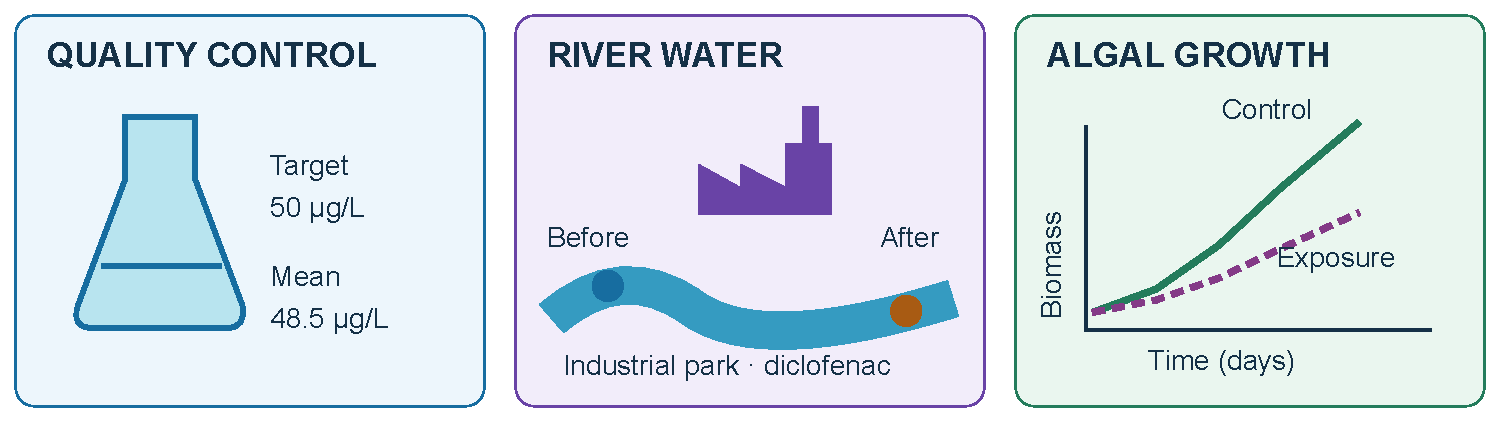
\includegraphics[width=\linewidth,height=.62\textheight,keepaspectratio]{asset-46dbeff25c887347aef9e80356c19be9d7383f12849554ad6fe9f5c23a3384c7.pdf}\end{center}

\medskip

\par\medskip
\Needspace{10cm}
\refstepcounter{figure}\label{material-09be8a5bf377d18d2d3eaa96b6e56c465ee991b2293cfb94299f0e8f37cf0fb5}
\noindent\textbf{Fig.~\ref*{material-09be8a5bf377d18d2d3eaa96b6e56c465ee991b2293cfb94299f0e8f37cf0fb5}.} From population claim to reference prediction, statistic and fallible decision.\par\nopagebreak
\begin{center}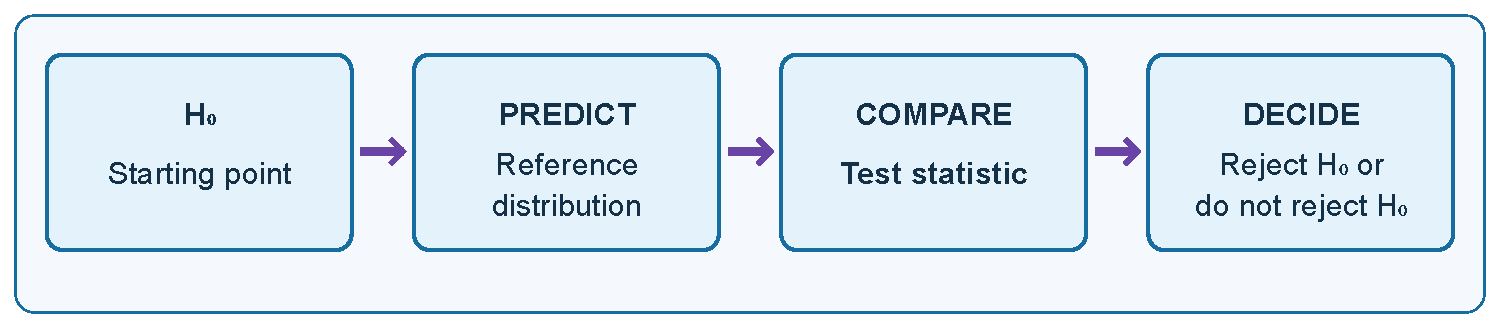
\includegraphics[width=\linewidth,height=.62\textheight,keepaspectratio]{asset-b6294fa05a0a2c323ee0cbec02bd29fc01bb4feaa956c23ae594536f88ce083b.pdf}\end{center}

\medskip

The single tree in \hyperref[material-89018b0eb50a0538f5720b37f8b519a81c9a106c8de06e70f47beec73f5fc8e3]{Fig.~\ref*{material-89018b0eb50a0538f5720b37f8b519a81c9a106c8de06e70f47beec73f5fc8e3}} starts with \textbf{H\ensuremath{{}_0}: \ensuremath{\mu} \ensuremath{\le} L}, where \ensuremath{\mu} is the population mean and L is the reference. \textbf{Positive} means rejecting H\ensuremath{{}_0} and claiming an exceedance; \textbf{negative} means not rejecting H\ensuremath{{}_0}. The thumbnails distinguish true positive, false positive (type I), false negative (type II), and true negative. Non-rejection cannot prove H\ensuremath{{}_0}. The three lake hypotheses serve different applications. An equality-only GO policy treats thicker ice as a departure too; non-rejection cannot establish exact equality. Match the burden of evidence to the consequences of an error.


\par\medskip
\Needspace{10cm}
\refstepcounter{figure}\label{material-89018b0eb50a0538f5720b37f8b519a81c9a106c8de06e70f47beec73f5fc8e3}
\noindent\textbf{Fig.~\ref*{material-89018b0eb50a0538f5720b37f8b519a81c9a106c8de06e70f47beec73f5fc8e3}.} One tree with positive/negative decisions and all four outcomes.\par\nopagebreak
\begin{center}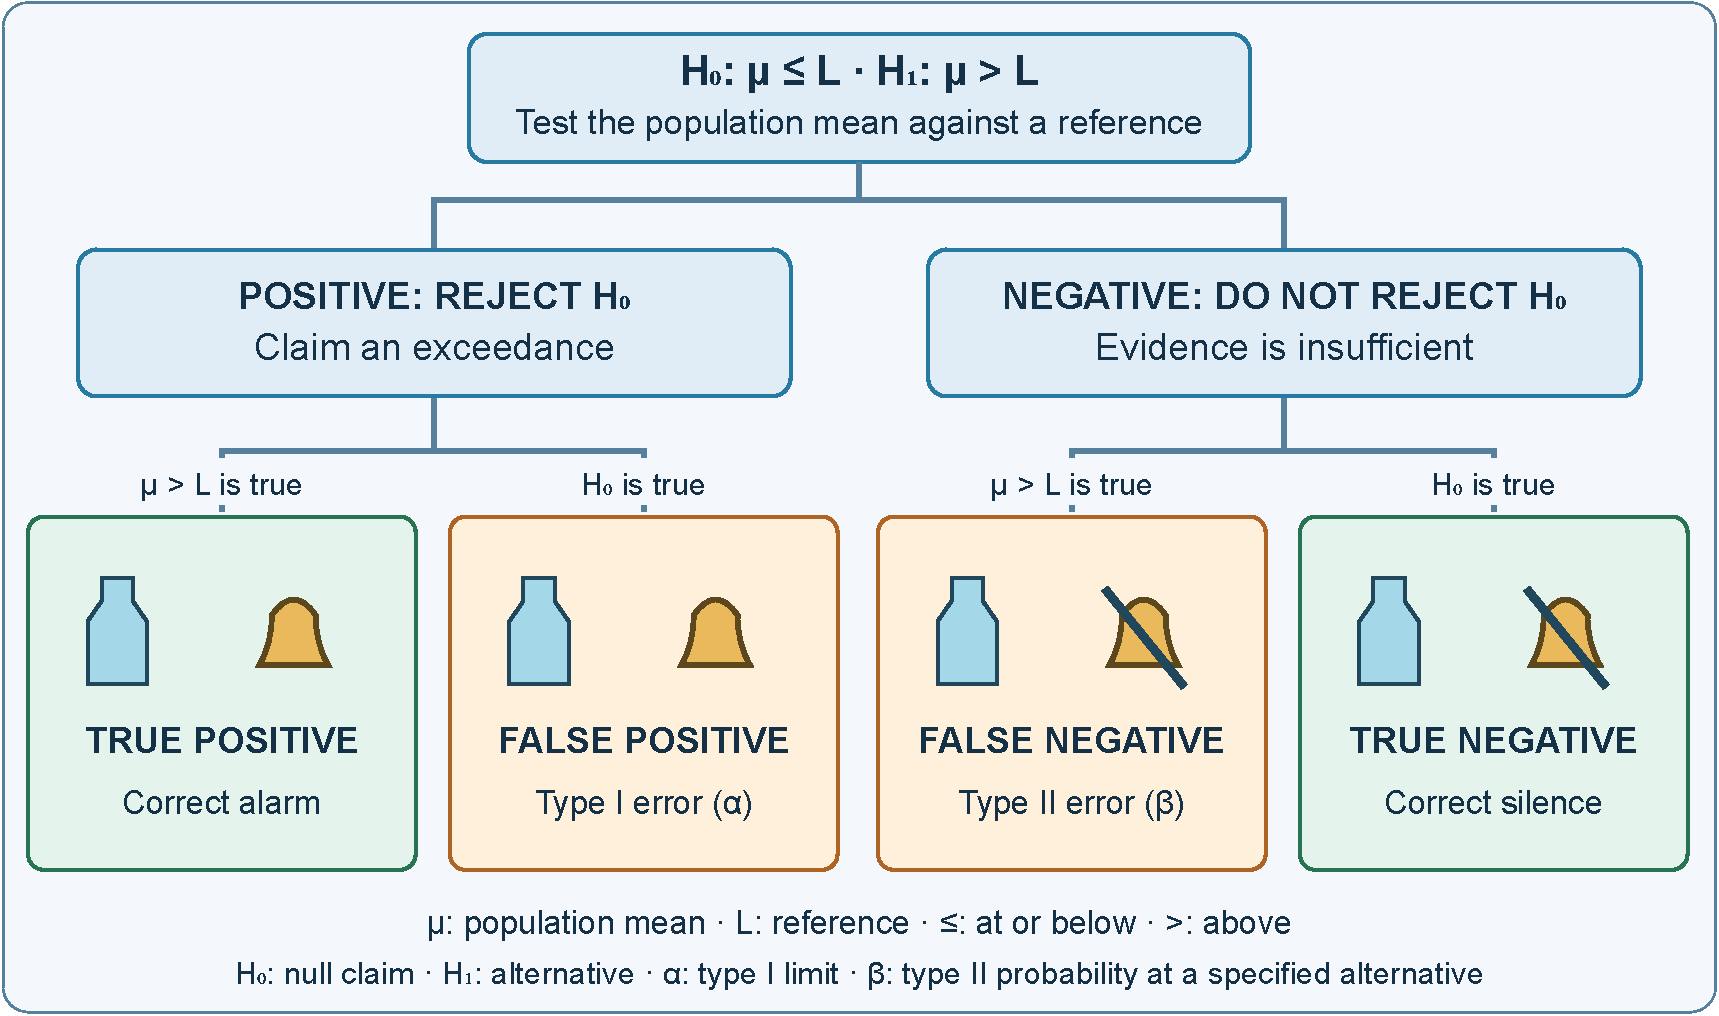
\includegraphics[width=\linewidth,height=.62\textheight,keepaspectratio]{asset-f0cb39ac1453592c0113f2c7e12fab49764d225bc0b0f3783060d13baa3669a1.pdf}\end{center}

\medskip

The lake illustration \hyperref[material-bfb49ae48ebc8d54f8288bcc325ff40d1098b8070f4df21fef841c45e94454d4]{Fig.~\ref*{material-bfb49ae48ebc8d54f8288bcc325ff40d1098b8070f4df21fef841c45e94454d4}} is a thought experiment about that burden of evidence, not crossing advice. Rule A starts with thickness at or below a hypothetical minimum and goes only after rejection. Rule B starts with thickness at or above the minimum and goes on non-rejection. For the same known-SD Normal measurement model, the decision probabilities in \hyperref[material-bbf4fde513faa7a5c1497146a4af0765e15ed8b95544235c20a2550bd8b967ff]{Fig.~\ref*{material-bbf4fde513faa7a5c1497146a4af0765e15ed8b95544235c20a2550bd8b967ff}} differ sharply. With four independent readings, population SD 0.5 cm and a 10 cm boundary, sample-mean SE is 0.25 cm. One-sided alpha 5\% gives GO thresholds 10.411 cm for A and 9.589 cm for B. At true 9.7 cm, GO occurs about 0.22\% versus 67.18\%; at true 10.3 cm, about 32.82\% versus 99.78\%. These compare repeated studies at the same true state, not two analyses producing different physical collapse probabilities from one observed mean. Real ice has local weak spots and other hazards not represented by this model.


\par\medskip
\Needspace{10cm}
\refstepcounter{figure}\label{material-bfb49ae48ebc8d54f8288bcc325ff40d1098b8070f4df21fef841c45e94454d4}
\noindent\textbf{Fig.~\ref*{material-bfb49ae48ebc8d54f8288bcc325ff40d1098b8070f4df21fef841c45e94454d4}.} Lake decision rules in a statistical thought experiment.\par\nopagebreak
\begin{center}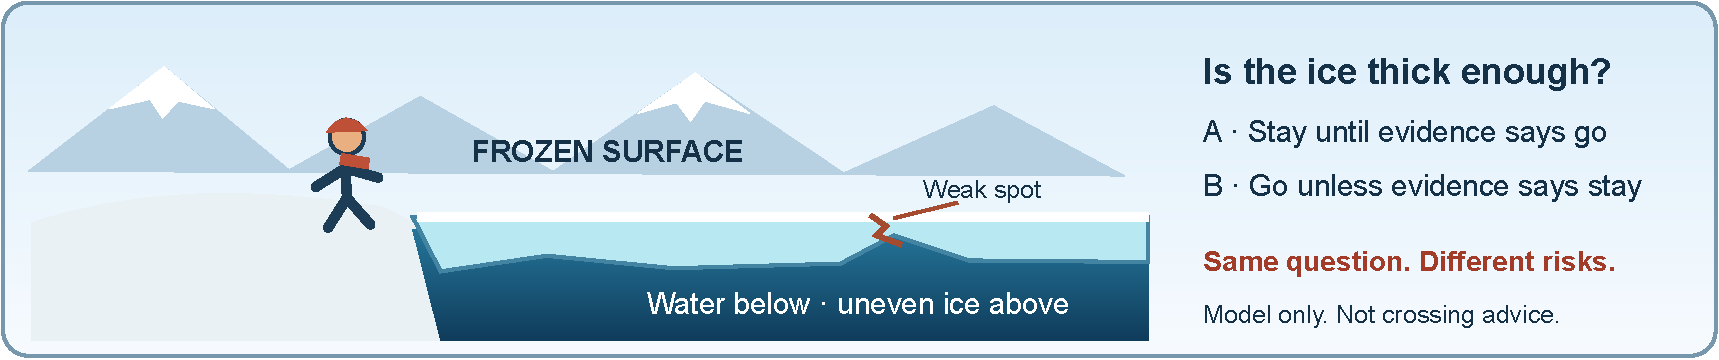
\includegraphics[width=\linewidth,height=.62\textheight,keepaspectratio]{asset-a7eb9161eb17e1782cbcc96ba9580fcdadf4ae74fd76dd4e407e300f58ef1943.pdf}\end{center}

\medskip

\par\medskip
\Needspace{10cm}
\refstepcounter{figure}\label{material-bbf4fde513faa7a5c1497146a4af0765e15ed8b95544235c20a2550bd8b967ff}
\noindent\textbf{Fig.~\ref*{material-bbf4fde513faa7a5c1497146a4af0765e15ed8b95544235c20a2550bd8b967ff}.} Comic: Normal-model GO probabilities at two true thicknesses.\par\nopagebreak
\begin{center}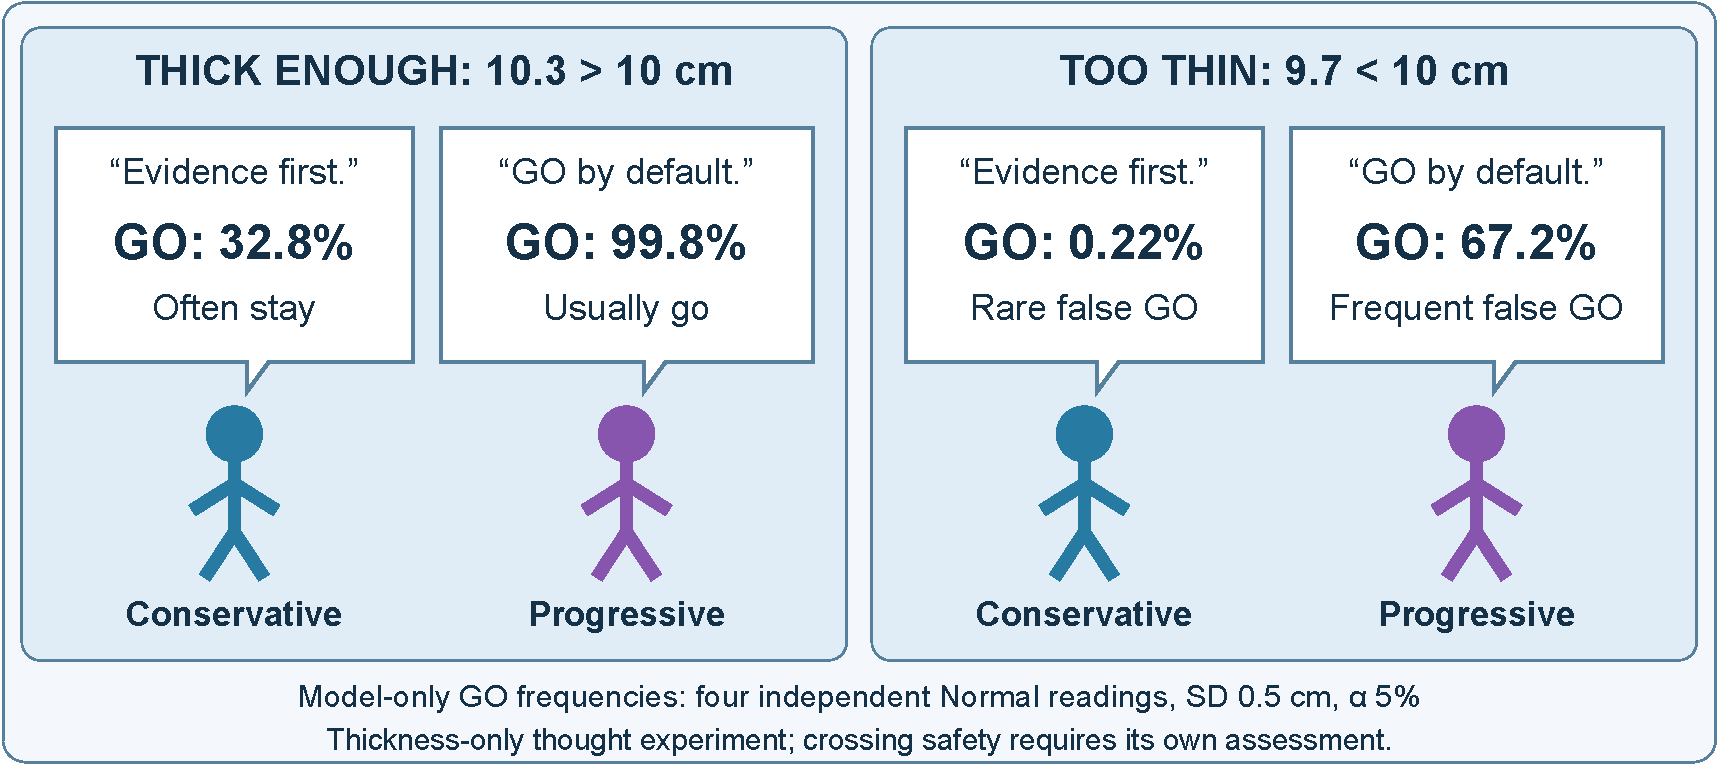
\includegraphics[width=\linewidth,height=.62\textheight,keepaspectratio]{asset-e2fe6449e91e05fc7d20a83f315a1ff7987d0a0da2e9a921e747b8ede92118e5.pdf}\end{center}

\medskip

\clearpage
\section{Error levels, degrees of freedom and p-values}
Choose alpha before observing the relevant outcomes. It bounds the procedure's false-rejection probability under H\ensuremath{{}_0} and the sampling model. Lower alpha is not a free improvement: with the same number of observations, variability and true departure, it can increase missed differences. The interactive amoxicillin example \hyperref[material-590d2fa56fb7cdcb0d21b3f9e412720a51bad473a868dc90f71874f1f7025cb9]{Fig.~\ref*{material-590d2fa56fb7cdcb0d21b3f9e412720a51bad473a868dc90f71874f1f7025cb9}} reuses 4000 seeded Normal-sample studies at a fixed true mean 1.4 µg/L versus teaching limit 1 µg/L. Ten independent results and population SD 0.5 µg/L define the model. The readouts distinguish worst-case type I error from simulated type II error.


\par\medskip
\Needspace{10cm}
\refstepcounter{figure}\label{material-590d2fa56fb7cdcb0d21b3f9e412720a51bad473a868dc90f71874f1f7025cb9}
\noindent\textbf{Fig.~\ref*{material-590d2fa56fb7cdcb0d21b3f9e412720a51bad473a868dc90f71874f1f7025cb9}.} Alpha slider: a reference curve and type I/type II readouts; simulation settings are fixed.\par\nopagebreak
\begin{center}
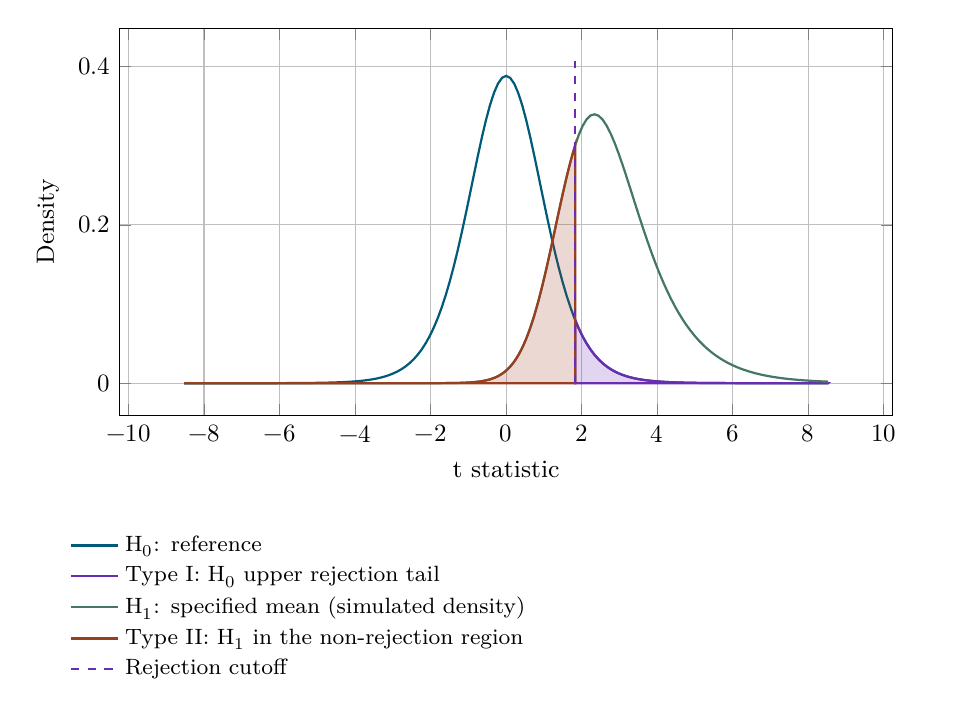
\begin{tikzpicture}
\begin{axis}[width=0.94\linewidth,
height=6.5cm,
scale only axis=false,
grid=major,
tick label style={font=\small},
label style={font=\small},
xlabel={t statistic},
ylabel={Density},
legend style={font=\footnotesize,draw=none,at={(0.5,-0.28)},anchor=north,legend columns=1,text width=0.85\linewidth,align=left},
unbounded coords=jump,
scaled ticks=false]
\addplot[color=pcd1,thick,mark=none] coordinates {(-8.529822128134704,0.000006272427082092728) (-8.42319935153302,0.000007014281659931123) (-8.316576574931336,0.000007852524424127219) (-8.209953798329652,0.000008800788505643127) (-8.10333102172797,0.000009874789518395798) (-7.996708245126285,0.000011092666659459104) (-7.890085468524601,0.000012475383324649805) (-7.783462691922917,0.000014047198231476203) (-7.676839915321233,0.00001583622017682908) (-7.57021713871955,0.000017875062125672622) (-7.463594362117866,0.00002020161342061371) (-7.356971585516182,0.000022859952631619526) (-7.250348808914499,0.000025901428065442984) (-7.143726032312815,0.000029385938390033607) (-7.037103255711131,0.000033383452400748355) (-6.9304804791094465,0.0000379758149066525) (-6.823857702507763,0.00004325889534398672) (-6.717234925906079,0.00004934514739221849) (-6.610612149304396,0.000056366662017052955) (-6.503989372702712,0.00006447881353115388) (-6.397366596101028,0.00007386461909986191) (-6.290743819499344,0.00008473995741881108) (-6.18412104289766,0.00009735982301478499) (-6.077498266295977,0.00011202582993484823) (-5.970875489694293,0.00012909522389825258) (-5.864252713092609,0.00014899171698481924) (-5.757629936490925,0.00017221852565533376) (-5.651007159889241,0.00019937407377261044) (-5.544384383287557,0.0002311709202018524) (-5.437761606685874,0.00026845858892050233) (-5.33113883008419,0.00031225112234405957) (-5.224516053482506,0.00036376035038400607) (-5.117893276880823,0.0004244360738553666) (-5.011270500279139,0.000496014607132939) (-4.904647723677455,0.0005805774178461237) (-4.798024947075771,0.0006806219476716831) (-4.691402170474087,0.0007991471046715072) (-4.584779393872403,0.0009397563902219832) (-4.478156617270719,0.0011067821668642671) (-4.371533840669036,0.0013054351887399592) (-4.264911064067352,0.0015419841997530537) (-4.158288287465668,0.00182397114390018) (-4.051665510863985,0.0021604683022385116) (-3.9450427342623007,0.002562384427837367) (-3.8384199576606166,0.0030428276231095844) (-3.7317971810589325,0.0036175331852053103) (-3.6251744044572494,0.0043053647762379115) (-3.5185516278555653,0.005128896830918559) (-3.4119288512538812,0.006115084784236202) (-3.305306074652198,0.007296027070049071) (-3.198683298050514,0.008709818366829145) (-3.092060521448831,0.010401486569372132) (-2.9854377448471467,0.012423995624830542) (-2.8788149682454627,0.014839281749994451) (-2.7721921916437786,0.017719270651194975) (-2.6655694150420945,0.02114679727424095) (-2.5589466384404114,0.025216316675690416) (-2.4523238618387273,0.030034254792807805) (-2.345701085237044,0.035718802236521664) (-2.23907830863536,0.042398905464450534) (-2.132455532033676,0.05021216294758231) (-2.025832755431992,0.05930129752547116) (-1.9192099788303079,0.06980886210177253) (-1.8125872022286247,0.08186986008368807) (-1.7059644256269406,0.09560204352075068) (-1.5993416490252574,0.11109381064361473) (-1.4927188724235734,0.1283898771273493) (-1.3860960958218893,0.14747524916696153) (-1.2794733192202061,0.16825847121752094) (-1.172850542618522,0.19055562106191037) (-1.0662277660168389,0.2140770116112606) (-0.9596049894151548,0.23841893160664157) (-0.8529822128134708,0.2630628915521972) (-0.7463594362117858,0.2873846101214449) (-0.6397366596101026,0.3106742852259854) (-0.5331138830084186,0.33216852082169823) (-0.4264911064067345,0.351092711847965) (-0.3198683298050504,0.36671093644679686) (-0.21324555320336813,0.37837878387870705) (-0.10662277660168407,0.3855934227920502) (0,0.38803490887166797) (0.10662277660168407,0.3855934227920502) (0.21324555320336813,0.37837878387870705) (0.3198683298050504,0.36671093644679686) (0.4264911064067345,0.351092711847965) (0.5331138830084186,0.33216852082169823) (0.6397366596101026,0.3106742852259854) (0.7463594362117867,0.2873846101214447) (0.8529822128134708,0.2630628915521972) (0.9596049894151548,0.23841893160664157) (1.0662277660168389,0.2140770116112606) (1.172850542618523,0.1905556210619101) (1.2794733192202052,0.16825847121752113) (1.3860960958218893,0.14747524916696153) (1.4927188724235734,0.1283898771273493) (1.5993416490252574,0.11109381064361473) (1.7059644256269415,0.0956020435207506) (1.8125872022286238,0.08186986008368823) (1.9192099788303079,0.06980886210177253) (2.025832755431992,0.05930129752547116) (2.132455532033676,0.05021216294758231) (2.23907830863536,0.042398905464450534) (2.3457010852370423,0.03571880223652176) (2.4523238618387264,0.030034254792807857) (2.5589466384404105,0.025216316675690464) (2.6655694150420963,0.021146797274240875) (2.7721921916437786,0.017719270651194975) (2.8788149682454627,0.014839281749994451) (2.9854377448471467,0.012423995624830542) (3.092060521448831,0.010401486569372132) (3.198683298050515,0.008709818366829138) (3.305306074652197,0.007296027070049084) (3.4119288512538812,0.006115084784236202) (3.5185516278555653,0.005128896830918559) (3.6251744044572494,0.0043053647762379115) (3.7317971810589334,0.003617533185205304) (3.8384199576606157,0.0030428276231095897) (3.9450427342623,0.002562384427837372) (4.051665510863984,0.0021604683022385133) (4.158288287465668,0.00182397114390018) (4.264911064067352,0.0015419841997530537) (4.371533840669034,0.0013054351887399627) (4.47815661727072,0.0011067821668642652) (4.584779393872402,0.0009397563902219841) (4.691402170474088,0.0007991471046715065) (4.7980249470757705,0.0006806219476716841) (4.904647723677455,0.0005805774178461237) (5.011270500279137,0.0004960146071329403) (5.117893276880823,0.0004244360738553666) (5.224516053482507,0.00036376035038400575) (5.331138830084189,0.0003122511223440601) (5.437761606685875,0.00026845858892050233) (5.544384383287557,0.0002311709202018524) (5.651007159889243,0.00019937407377261008) (5.757629936490925,0.00017221852565533376) (5.864252713092609,0.00014899171698481924) (5.970875489694292,0.0001290952238982528) (6.077498266295978,0.00011202582993484803) (6.18412104289766,0.00009735982301478499) (6.290743819499344,0.00008473995741881108) (6.397366596101026,0.00007386461909986204) (6.503989372702712,0.00006447881353115388) (6.610612149304394,0.000056366662017053056) (6.71723492590608,0.0000493451473922184) (6.8238577025077625,0.00004325889534398672) (6.9304804791094465,0.0000379758149066525) (7.037103255711132,0.000033383452400748294) (7.143726032312815,0.000029385938390033607) (7.250348808914499,0.000025901428065442984) (7.356971585516181,0.000022859952631619526) (7.463594362117867,0.00002020161342061371) (7.570217138719549,0.000017875062125672622) (7.676839915321235,0.000015836220176829025) (7.783462691922917,0.000014047198231476203) (7.890085468524603,0.000012475383324649783) (7.996708245126285,0.000011092666659459104) (8.103331021727968,0.000009874789518395816) (8.20995379832965,0.000008800788505643143) (8.316576574931336,0.000007852524424127219) (8.423199351533018,0.000007014281659931148) (8.529822128134704,0.000006272427082092728)};
\addlegendentry{H\ensuremath{{}_0}: reference}
\addplot[color=pcd2,thick,mark=none,fill=pcd2,fill opacity=0.2] coordinates {(1.8331129326562343,0.07942143963996284) (1.8749673651279748,0.074617701608594) (1.9168217975997153,0.07006152246524647) (1.9586762300714555,0.0657453450019254) (2.0005306625431962,0.06166120474031647) (2.0423850950149367,0.05780082763335718) (2.0842395274866767,0.054155718835520505) (2.126093959958417,0.05071724270698546) (2.1679483924301577,0.04747669431555837) (2.209802824901898,0.04442536277924931) (2.2516572573736386,0.04155458685350077) (2.293511689845379,0.03885580321202391) (2.3353661223171196,0.03632058790087048) (2.3772205547888596,0.03394069146359083) (2.4190749872606006,0.031708068242877585) (2.4609294197323406,0.02961490036265082) (2.5027838522040815,0.02765361688567382) (2.5446382846758215,0.025816908626936502) (2.586492717147562,0.024097739083498614) (2.6283471496193025,0.02248935191840489) (2.670201582091043,0.020985275410675353) (2.7120560145627834,0.019579324256113854) (2.753910447034524,0.018265599075505477) (2.7957648795062644,0.017038483958314993) (2.8376193119780044,0.01589264234176132) (2.8794737444497454,0.01482301149754266) (2.9213281769214854,0.013824795871842006) (2.9631826093932263,0.012893459498800596) (3.0050370418649663,0.0120247176835841) (3.046891474336707,0.011214528128599813) (3.0887459068084473,0.010459081655427471) (3.1306003392801878,0.009754792655627877) (3.1724547717519282,0.009098289385792468) (3.2143092042236683,0.0084864042059634) (3.256163636695409,0.007916163845838091) (3.2980180691671492,0.007384779769910726) (3.33987250163889,0.006889638700818993) (3.38172693411063,0.006428293349575029) (3.423581366582371,0.005998453391976195) (3.465435799054111,0.005597976722225003) (3.5072902315258516,0.005224861007546907) (3.549144663997592,0.004877235561293233) (3.590999096469332,0.004553353546565811) (3.632853528941073,0.004251584517720596) (3.6747079614128135,0.0039704073031195915) (3.716562393884554,0.0037084032291318453) (3.758416826356294,0.003464249682566702) (3.8002712588280345,0.003236714006392461) (3.842125691299775,0.003024647721693675) (3.8839801237715155,0.002826981067296927) (3.925834556243256,0.0026427178473001495) (3.9676889887149964,0.0024709305758308037) (4.009543421186736,0.0023107559076939775) (4.051397853658477,0.0021613903431178592) (4.093252286130218,0.0020220861945294635) (4.135106718601958,0.0018921478031702858) (4.176961151073698,0.0017709279933648579) (4.218815583545439,0.00165782475236369) (4.26067001601718,0.0015522781238763443) (4.30252444848892,0.0014537673036742063) (4.34437888096066,0.0013618079259614248) (4.386233313432401,0.001275949529573949) (4.428087745904142,0.0011957731934599744) (4.469942178375881,0.0011208893313114639) (4.511796610847622,0.001050935635647684) (4.553651043319363,0.0009855751620917162) (4.595505475791103,0.0009244945450237628) (4.637359908262843,0.0008674023362367858) (4.679214340734584,0.0008140274586563407) (4.721068773206325,0.0007641177676147768) (4.762923205678065,0.0007174387125875874) (4.804777638149805,0.0006737720927050485) (4.8466320706215456,0.0006329148997436006) (4.8884865030932865,0.0005946782426779693) (4.930340935565026,0.0005588863482358632) (4.9721953680367665,0.0005253756322419592) (5.0140498005085075,0.0004939938368664389) (5.0559042329802475,0.00046459922920556913) (5.0977586654519875,0.0004370598569180063) (5.1396130979237284,0.0004112528569206609) (5.181467530395469,0.00038706381341265824) (5.2233219628672085,0.00036438616174548795) (5.265176395338949,0.0003431206348923993) (5.30703082781069,0.00032317474949098893) (5.34888526028243,0.00030446232864031513) (5.390739692754171,0.00028690305882838615) (5.432594125225911,0.00027042207854804977) (5.474448557697652,0.00025494959632982436) (5.516302990169393,0.0002404205360796399) (5.558157422641132,0.00022677420775834648) (5.600011855112873,0.0002139540015789017) (5.641866287584613,0.00020190710402678353) (5.683720720056354,0.0001905842341300485) (5.725575152528094,0.00017993939851806414) (5.767429584999835,0.00016992966391276602) (5.809284017471576,0.0001605149457938619) (5.851138449943315,0.00015165781207013876) (5.892992882415056,0.00014332330067339582) (5.934847314886797,0.0001354787500699475) (5.976701747358538,0.0001280936417574616) (6.018556179830277,0.00012113945388256548) (6.060410612302018,0.00011458952517745436) (6.102265044773759,0.00010841892847203706) (6.144119477245498,0.00010260435309224222) (6.185973909717239,0.00009712399550530562) (6.22782834218898,0.00009195745761940731) (6.269682774660721,0.0000870856521881902) (6.31153720713246,0.00008249071481073045) (6.353391639604201,0.00007815592205463189) (6.395246072075942,0.00007406561526432224) (6.437100504547681,0.00007020512964850753) (6.478954937019422,0.00006656072827029558) (6.520809369491163,0.00006311954059088638) (6.562663801962904,0.00005986950524309336) (6.604518234434645,0.00005679931673448658) (6.646372666906384,0.00005389837580172555) (6.688227099378125,0.00005115674315784414) (6.730081531849866,0.000048565096392949646) (6.771935964321605,0.00004611468980613204) (6.813790396793346,0.00004379731696243466) (6.855644829265087,0.00004160527578361747) (6.897499261736828,0.00003953133599522863) (6.939353694208567,0.00003756870876527652) (6.981208126680308,0.0000357110183816298) (7.023062559152049,0.00003395227582624576) (7.064916991623788,0.00003228685411449083) (7.106771424095529,0.000030709465277242204) (7.14862585656727,0.00002921513887219297) (7.1904802890390105,0.000027799201918877454) (7.23233472151075,0.000026457260159441225) (7.2741891539824906,0.000025185180554135814) (7.3160435864542315,0.00002397907492697369) (7.357898018925971,0.000022835284682957974) (7.3997524513977115,0.000021750366523852854) (7.4416068838694525,0.0000207210790946059) (7.483461316341193,0.00001974437049730824) (7.5253157488129325,0.000018817366614005694) (7.5671701812846734,0.000017937360183785332) (7.609024613756414,0.00001710180058337469) (7.6508790462281535,0.000016308284264028437) (7.692733478699894,0.00001555454580076454) (7.734587911171635,0.000014838449513060239) (7.776442343643376,0.000014157981618949542) (7.818296776115117,0.000013511242887093803) (7.860151208586856,0.000012896441753838716) (7.902005641058597,0.000012311887874538512) (7.943860073530338,0.000011755986080536898) (7.985714506002077,0.000011227230715150578) (8.027568938473818,0.000010724200323821524) (8.06942337094556,0.00001024555267529547) (8.1112778034173,0.00000979002009225595) (8.15313223588904,0.00000935640507130401) (8.19498666836078,0.000008943576173534909) (8.236841100832521,0.000008550464168225158) (8.27869553330426,0.000008176058413320021) (8.320549965776001,0.000007819403457505985) (8.362404398247742,0.000007479595849670119) (8.404258830719483,0.000007155781142495325) (8.446113263191224,0.000006847151077823796) (8.487967695662963,0.000006552940942240312) (8.529822128134704,0.000006272427082092728)} \closedcycle;
\addlegendentry{Type I: H\ensuremath{{}_0} upper rejection tail}
\addplot[color=pcd3,thick,mark=none] coordinates {(-8.529822128134704,6.214985755351244e-11) (-8.42319935153302,7.667275799010107e-11) (-8.316576574931336,9.453679286775311e-11) (-8.209953798329652,1.165003240519137e-10) (-8.10333102172797,1.4349204996372487e-10) (-7.996708245126285,1.7664902993515013e-10) (-7.890085468524601,2.173631971936274e-10) (-7.783462691922917,2.6733827246926025e-10) (-7.676839915321233,3.286594300350521e-10) (-7.57021713871955,4.038786126933083e-10) (-7.463594362117866,4.961190681419923e-10) (-7.356971585516182,6.092035196633668e-10) (-7.250348808914499,7.47811431586727e-10) (-7.143726032312815,9.176721385543393e-10) (-7.037103255711131,1.1258022463935294e-9) (-6.9304804791094465,1.3807977700162614e-9) (-6.823857702507763,1.6931940642419996e-9) (-6.717234925906079,2.075909873825258e-9) (-6.610612149304396,2.5447959694770045e-9) (-6.503989372702712,3.119314094009393e-9) (-6.397366596101028,3.8233786377614464e-9) (-6.290743819499344,4.686402013553618e-9) (-6.18412104289766,5.744595655497324e-9) (-6.077498266295977,7.042592639809351e-9) (-5.970875489694293,8.635476060955704e-9) (-5.864252713092609,1.0591320732918465e-8) (-5.757629936490925,1.299438615979375e-8) (-5.651007159889241,1.5949138197594523e-8) (-5.544384383287557,1.9585328281474718e-8) (-5.437761606685874,2.40644263363051e-8) (-5.33113883008419,2.958779160883623e-8) (-5.224516053482506,3.6407081448284325e-8) (-5.117893276880823,4.483755061245218e-8) (-5.011270500279139,5.527509519464851e-8) (-4.904647723677455,6.821816218067533e-8) (-4.798024947075771,8.429600012572416e-8) (-4.691402170474087,1.0430519849442477e-7) (-4.584779393872403,1.292570935649492e-7) (-4.478156617270719,1.604394629198991e-7) (-4.371533840669036,1.9949706418636482e-7) (-4.264911064067352,2.4853710065578724e-7) (-4.158288287465668,3.1026775944460866e-7) (-4.051665510863985,3.8818076386162096e-7) (-3.9450427342623007,4.867926832051438e-7) (-3.8384199576606166,6.119649289087363e-7) (-3.7317971810589325,7.713294633355383e-7) (-3.6251744044572494,9.748569940175169e-7) (-3.5185516278555653,0.0000012356178555738133) (-3.4119288512538812,0.0000015708043470837816) (-3.305306074652198,0.0000020031090414547335) (-3.198683298050514,0.000002562589404057775) (-3.092060521448831,0.000003289199031217918) (-2.9854377448471467,0.0000042362357105147414) (-2.8788149682454627,0.00000547505445391305) (-2.7721921916437786,0.00000710153113005472) (-2.6655694150420945,0.000009244955426912143) (-2.5589466384404114,0.000012080303104422754) (-2.4523238618387273,0.00001584521804111449) (-2.345701085237044,0.000020863567268762952) (-2.23907830863536,0.000027578175068382387) (-2.132455532033676,0.000036596372584292594) (-2.025832755431992,0.000048753417949243464) (-1.9192099788303079,0.00006520077560785652) (-1.8125872022286247,0.00008752884573671415) (-1.7059644256269406,0.0001179371786186303) (-1.5993416490252574,0.00015946966911934487) (-1.4927188724235734,0.0002163378400946646) (-1.3860960958218893,0.0002943621195285291) (-1.2794733192202061,0.0004015687990138416) (-1.172850542618522,0.000548988535638576) (-1.0662277660168389,0.0007517095885703099) (-0.9596049894151548,0.0010302432884833788) (-0.8529822128134708,0.0014122570928965152) (-0.7463594362117858,0.0019347170731807755) (-0.6397366596101026,0.0026464504440792394) (-0.5331138830084186,0.0036110824940567016) (-0.4264911064067345,0.004910214133021611) (-0.3198683298050504,0.006646582229689392) (-0.21324555320336813,0.008946787442662548) (-0.10662277660168407,0.011962996802548762) (0,0.015872859501263905) (0.10662277660168407,0.02087675989624318) (0.21324555320336813,0.027191531259903333) (0.3198683298050504,0.03503993001521812) (0.4264911064067345,0.04463556978717791) (0.5331138830084186,0.0561636439178634) (0.6397366596101026,0.06975856844251051) (0.7463594362117867,0.08548052894468665) (0.8529822128134708,0.10329363273387383) (0.9596049894151548,0.1230487553497695) (1.0662277660168389,0.14447407086835842) (1.172850542618523,0.16717560619353972) (1.2794733192202052,0.19064902190679084) (1.3860960958218893,0.21430237568015686) (1.4927188724235734,0.23748812483531587) (1.5993416490252574,0.2595413436728024) (1.7059644256269415,0.27982029360220945) (1.8125872022286238,0.2977452232281042) (1.9192099788303079,0.3128316125591402) (2.025832755431992,0.3247149233514088) (2.132455532033676,0.33316510526260307) (2.23907830863536,0.3380904186206496) (2.3457010852370423,0.3395313528300067) (2.4523238618387264,0.33764637092081934) (2.5589466384404105,0.3326917938951421) (2.6655694150420963,0.3249983337410074) (2.7721921916437786,0.3149466426744301) (2.8788149682454627,0.30294386498844766) (2.9854377448471467,0.28940266820420857) (3.092060521448831,0.27472369232923644) (3.198683298050515,0.25928186377278406) (3.305306074652197,0.24341661695680566) (3.4119288512538812,0.22742576819402202) (3.5185516278555653,0.2115625903451809) (3.6251744044572494,0.19603552971397442) (3.7317971810589334,0.18100997079976353) (3.8384199576606157,0.16661147172068713) (3.9450427342623,0.1529299467674644) (4.051665510863984,0.14002434843145398) (4.158288287465668,0.127927487657157) (4.264911064067352,0.116650718753287) (4.371533840669034,0.10618829749647139) (4.47815661727072,0.09652129288357772) (4.584779393872402,0.08762099220654741) (4.691402170474088,0.07945178487206922) (4.7980249470757705,0.07197354326446627) (4.904647723677455,0.06514354047282113) (5.011270500279137,0.058917956890759536) (5.117893276880823,0.053253032711261965) (5.224516053482507,0.048105923224284995) (5.331138830084189,0.043435310349537626) (5.437761606685875,0.03920181841801157) (5.544384383287557,0.03536827591427331) (5.651007159889243,0.03189985844531113) (5.757629936490925,0.028764142082940213) (5.864252713092609,0.025931090702983252) (5.970875489694292,0.023372996136496776) (6.077498266295978,0.021064385878751337) (6.18412104289766,0.018981909732766235) (6.290743819499344,0.017104214025505965) (6.397366596101026,0.015411809842224284) (6.503989372702712,0.01388693999214961) (6.610612149304394,0.012513448066442407) (6.71723492590608,0.011276651905827856) (6.8238577025077625,0.010163222999430779) (6.9304804791094465,0.009161072737125096) (7.037103255711132,0.008259245993345026) (7.143726032312815,0.007447822196923843) (7.250348808914499,0.006717823811958097) (7.356971585516181,0.006061131997233905) (7.463594362117867,0.005470409109149424) (7.570217138719549,0.0049390276516464715) (7.676839915321235,0.00446100524563128) (7.783462691922917,0.004030945181240431) (7.890085468524603,0.003643982122487803) (7.996708245126285,0.003295732550221708) (8.103331021727968,0.0029822495520602102) (8.20995379832965,0.0026999815941811754) (8.316576574931336,0.0024457349374342823) (8.423199351533018,0.0022166393877572762) (8.529822128134704,0.0020101170973487255)};
\addlegendentry{H\ensuremath{{}_1}: specified mean (simulated density)}
\addplot[color=pcd4,thick,mark=none,fill=pcd4,fill opacity=0.2] coordinates {(-8.529822128134704,6.214985755351244e-11) (-8.46505378400476,7.061055279177286e-11) (-8.400285439874818,8.020639696524736e-11) (-8.335517095744875,9.108775654900131e-11) (-8.270748751614931,1.0342471281408887e-10) (-8.205980407484986,1.1740962939174695e-10) (-8.141212063355043,1.3326005367098165e-10) (-8.0764437192251,1.5122199567227232e-10) (-8.011675375095157,1.7157363383321154e-10) (-7.946907030965214,1.9462950372562985e-10) (-7.882138686835271,2.207452332105151e-10) (-7.817370342705327,2.5032289605626476e-10) (-7.752601998575384,2.838170657464166e-10) (-7.68783365444544,3.217416622566119e-10) (-7.623065310315496,3.6467769718532763e-10) (-7.558296966185553,4.1328203700745005e-10) (-7.49352862205561,4.682973206487821e-10) (-7.428760277925667,5.305631863590411e-10) (-7.363991933795724,6.010289843458654e-10) (-7.29922358966578,6.807681762342412e-10) (-7.234455245535837,7.709946506127348e-10) (-7.1696869014058935,8.730812162758535e-10) (-7.1049185572759495,9.885805719174158e-10) (-7.040150213146006,1.11924909372712e-9) (-6.975381869016063,1.2670738314703466e-9) (-6.91061352488612,1.4343031602164646e-9) (-6.845845180756177,1.6234816001233392e-9) (-6.781076836626233,1.8374893919889026e-9) (-6.71630849249629,2.0795875032899664e-9) (-6.6515401483663465,2.3534688400698537e-9) (-6.5867718042364025,2.6633165565742504e-9) (-6.522003460106459,3.013870489625072e-9) (-6.457235115976516,3.4105029014898985e-9) (-6.392466771846573,3.8593048971277125e-9) (-6.32769842771663,4.367185093501244e-9) (-6.262930083586686,4.941982365249524e-9) (-6.198161739456743,5.592594778438952e-9) (-6.1333933953268,6.3291271594752695e-9) (-6.068625051196856,7.163060137976815e-9) (-6.003856707066912,8.107443960440898e-9) (-5.939088362936969,9.177120907666646e-9) (-5.874320018807026,1.0388980777107977e-8) (-5.809551674677083,1.176225462819262e-8) (-5.744783330547139,1.3318852853841475e-8) (-5.680014986417196,1.5083754658340495e-8) (-5.615246642287253,1.7085457218166776e-8) (-5.550478298157309,1.9356494211464217e-8) (-5.4857099540273655,2.193403506302978e-8) (-5.420941609897422,2.486057821196348e-8) (-5.356173265767479,2.8184754024664936e-8) (-5.291404921637535,3.1962255713706173e-8) (-5.226636577507593,3.6256919863459235e-8) (-5.161868233377649,4.11419820021864e-8) (-5.097099889247706,4.6701537212611634e-8) (-5.032331545117762,5.303224117670828e-8) (-4.967563200987819,6.024529347112531e-8) (-4.902794856857875,6.846875256635475e-8) (-4.838026512727932,7.785024107481383e-8) (-4.773258168597989,8.856011062888413e-8) (-4.708489824468045,1.0079514869733064e-7) (-4.643721480338102,1.1478292508721834e-7) (-4.578953136208158,1.3078689433586599e-7) (-4.514184792078216,1.4911239228744297e-7) (-4.449416447948272,1.701136916155275e-7) (-4.3846481038183285,1.9420231279853446e-7) (-4.319879759688385,2.2185682517550353e-7) (-4.255111415558441,2.5363441853809305e-7) (-4.190343071428499,2.901845808734968e-7) (-4.125574727298555,3.3226528434104817e-7) (-4.060806383168612,3.807621617571847e-7) (-3.996038039038668,4.3671125273086586e-7) (-3.9312696949087247,5.013260157456687e-7) (-3.8665013507787815,5.760294443495844e-7) (-3.8017330066488384,6.6249229761486e-7) (-3.7369646625188953,7.626786638289864e-7) (-3.672196318388951,8.789003301609043e-7) (-3.607427974259008,0.0000010138817398836441) (-3.542659630129064,0.000001170837695024374) (-3.477891285999122,0.0000013535664213295455) (-3.4131229418691778,0.000001566561173008431) (-3.3483545977392346,0.000001815144240076871) (-3.2835862536092915,0.000002105628059920026) (-3.2188179094793474,0.000002445509162281458) (-3.154049565349405,0.00000284370193688472) (-3.089281221219461,0.0000033108207590976287) (-3.024512877089518,0.000003859520907759205) (-2.959744532959574,0.000004504911042153852) (-2.894976188829631,0.0000052650528725464565) (-2.8302078446996877,0.0000061615671839808545) (-2.7654395005697445,0.000007220369707264323) (-2.7006711564398014,0.000008472565658865318) (-2.6359028123098573,0.000009955538317835285) (-2.571134468179914,0.000011714275045990571) (-2.50636612404997,0.000013802984017646945) (-2.441597779920028,0.000016287067004258107) (-2.376829435790084,0.000019245528331968733) (-2.3120610916601407,0.0000227739181595193) (-2.2472927475301976,0.000026987930172662183) (-2.1825244034002536,0.00003202780043066334) (-2.1177560592703104,0.00003806368631751534) (-2.0529877151403664,0.00004530224334919783) (-1.9882193710104232,0.00005399466408318124) (-1.923451026880481,0.0000644464987730849) (-1.8586826827505378,0.00007702964296952011) (-1.7939143386205938,0.00009219695423799972) (-1.7291459944906507,0.00011050004968979345) (-1.6643776503607075,0.00013261093899432844) (-1.5996093062307635,0.00015934826440138362) (-1.5348409621008203,0.00019170904975742212) (-1.4700726179708763,0.0002309070031691851) (-1.4053042738409331,0.0002784185699064366) (-1.34053592971099,0.00033603808826864737) (-1.275767585581046,0.00040594355357175595) (-1.2109992414511037,0.0004907746326425769) (-1.1462308973211606,0.0005937246772896914) (-1.0814625531912174,0.0007186485388946856) (-1.0166942090612734,0.0008701879602140711) (-0.9519258649313302,0.001053916180779263) (-0.8871575208013862,0.0012765030983051292) (-0.8223891766714431,0.001545901833491108) (-0.7576208325414999,0.0018715567981078397) (-0.6928524884115559,0.002264632313031931) (-0.6280841442816127,0.0027382594131762535) (-0.5633158001516705,0.003307796668102569) (-0.49854745602172734,0.0039910986156375845) (-0.4337791118917842,0.0048087827535784064) (-0.3690107677618393,0.005784483003417628) (-0.30424242363189613,0.006945074243789547) (-0.23947407950195299,0.008320849067918471) (-0.17470573537200984,0.009945624579984791) (-0.1099373912420667,0.011856754118598342) (-0.045169047112121774,0.014095016662931373) (0.01959929701782137,0.016704355776920844) (0.08436764114776452,0.01973144074482212) (0.14913598527770588,0.023225025495217808) (0.2139043294076508,0.027235086372465515) (0.27867267353759395,0.03181172802315935) (0.3434410176675371,0.037003857636478336) (0.40820936179748024,0.04285764125394727) (0.4729777059274234,0.04941477127592027) (0.5377460500573683,0.05671059074887376) (0.6025143941873115,0.06477213634446603) (0.6672827383172546,0.07361617675907554) (0.7320510824471977,0.0832473351101943) (0.7968194265771409,0.09365639139357172) (0.861587770707084,0.10481886303722383) (0.9263561148370272,0.11669395727763056) (0.9911244589669703,0.12922397822650364) (1.0558928030969135,0.14233425439798417) (1.1206611472268584,0.15593362999642546) (1.1854294913568015,0.16991553679182195) (1.2501978354867447,0.18415963467519814) (1.3149661796166878,0.19853397994250152) (1.379734523746631,0.21289765298833815) (1.444502867876576,0.22710375324551874) (1.5092712120065173,0.24100265043972832) (1.5740395561364604,0.2544453686965352) (1.6388079002664035,0.26728697442497346) (1.7035762443963485,0.27938984039294723) (1.7683445885262916,0.2906266667002049) (1.8331129326562348,0.30088315369518637)} \closedcycle;
\addlegendentry{Type II: H\ensuremath{{}_1} in the non-rejection region}
\addplot[color=pcd2,dashed,thick] coordinates {(1.8331129326562343,0) (1.8331129326562343,0.4074366543152514)};
\addlegendentry{Rejection cutoff}
\end{axis}
\end{tikzpicture}
\end{center}

% Full-precision experiment details: {"blockId":"ex:l6-i05bc--block","parameters":[{"key":"alpha","label":"Alpha: allowed false-rejection risk","value":0.05},{"key":"view","label":"Error trade-off view","value":1},{"key":"n","label":"Independent measurements","value":10},{"key":"mean","label":"Reference mean (µg/L)","value":1},{"key":"sd","label":"Assumed population SD (µg/L)","value":0.5},{"key":"reference","label":"Teaching limit (µg/L)","value":1},{"key":"direction","label":"Upper-tail test","value":1},{"key":"effect","label":"True excess at the specified alternative (µg/L)","value":0.4},{"key":"M","label":"Simulated studies","value":4000},{"key":"seed","label":"Reproducible seed","value":617}],"readouts":[{"label":"Worst-case type I error (%)","value":5},{"label":"Simulated type II error (%)","value":25.124999999999996}],"note":"Same 4000 seeded independent Normal-sample studies at every alpha. True mean departure 0.4; assumed population SD 0.5; n = 10. Lower alpha shrinks the rejection region but increases missed differences for this fixed alternative. Beta is simulated, not a probability that H0 is true.","markers":[[{"x":1.8331129326562343,"label":"Rejection cutoff"}]]}

\medskip

Degrees of freedom, written \textbf{\ensuremath{\nu}} and pronounced nu, describe information remaining after fitting constraints. The residuals add to zero once their mean is fitted. Six independent observations therefore leave \textbf{\ensuremath{\nu} = 5} for an SD estimate. Fitting intercept and slope leaves \textbf{\ensuremath{\nu} = 4}, as illustrated in \hyperref[material-3bbbbe57323cb765051826879fff8a9e369555f5db791515cee83d589ab07619]{Fig.~\ref*{material-3bbbbe57323cb765051826879fff8a9e369555f5db791515cee83d589ab07619}}. In these full-rank models, each independently fitted coefficient costs one residual degree of freedom. Other references can use a fractional approximation.


\par\medskip
\Needspace{10cm}
\refstepcounter{figure}\label{material-3bbbbe57323cb765051826879fff8a9e369555f5db791515cee83d589ab07619}
\noindent\textbf{Fig.~\ref*{material-3bbbbe57323cb765051826879fff8a9e369555f5db791515cee83d589ab07619}.} Six observations with one fitted mean versus two fitted line coefficients.\par\nopagebreak
\begin{center}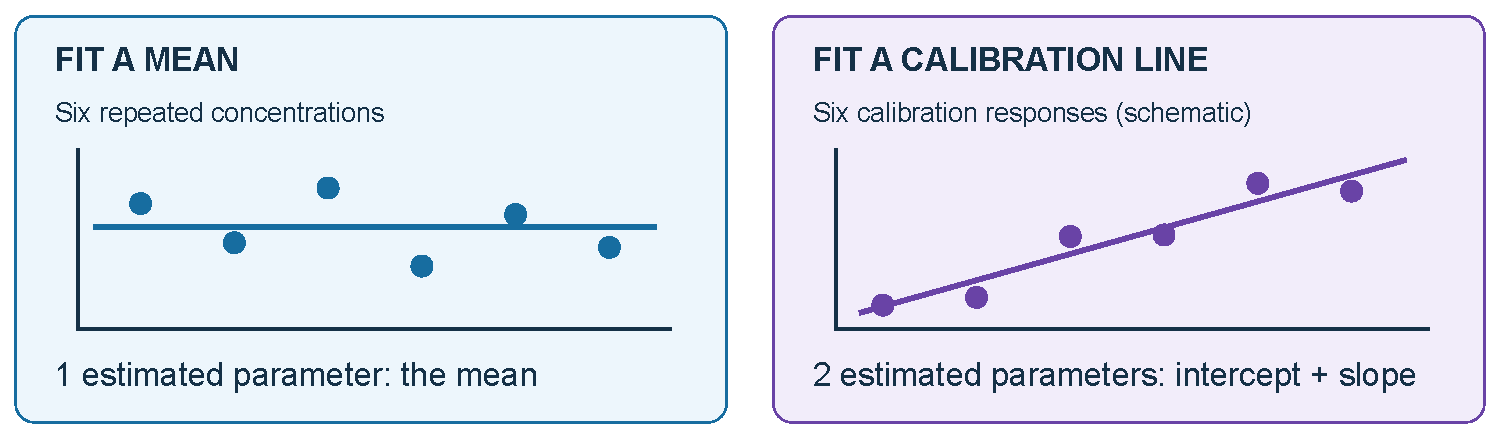
\includegraphics[width=\linewidth,height=.62\textheight,keepaspectratio]{asset-18b4f74888365cf4561aca91261518a043c8e76b26dbee8b8aad5759854cd0df.pdf}\end{center}

\medskip

A p-value is a probability conditional on H\ensuremath{{}_0} and the sampling model: a statistic at least as extreme as the one observed, in the planned direction. The upper tail in \hyperref[material-40c2a68631c0225187176e18496969a749a10bf4382a96f412154a999133a1e7]{Fig.~\ref*{material-40c2a68631c0225187176e18496969a749a10bf4382a96f412154a999133a1e7}} counts unusually high results for an exceedance question, with the null boundary used for calibration. Compare p with the alpha chosen in advance. Small p challenges the null model; it is not the probability that H\ensuremath{{}_0} is true, a measurement of effect size, or evidence of causal mechanism.


\par\medskip
\Needspace{10cm}
\refstepcounter{figure}\label{material-40c2a68631c0225187176e18496969a749a10bf4382a96f412154a999133a1e7}
\noindent\textbf{Fig.~\ref*{material-40c2a68631c0225187176e18496969a749a10bf4382a96f412154a999133a1e7}.} An observed upper-tail statistic and results at least as extreme under the null boundary.\par\nopagebreak
\begin{center}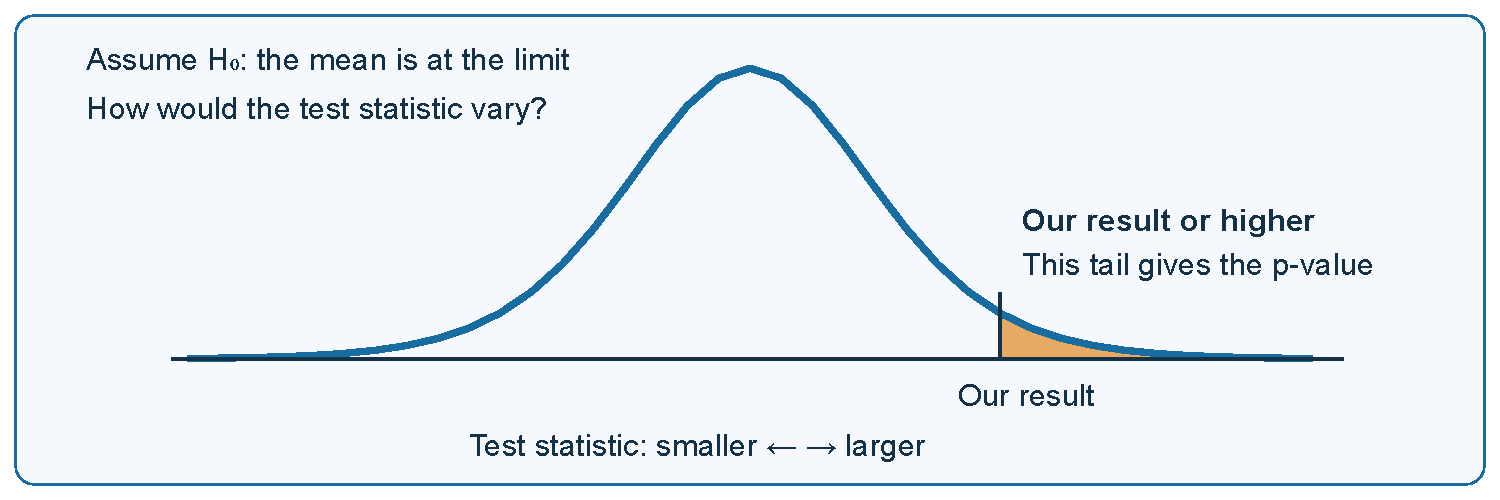
\includegraphics[width=\linewidth,height=.62\textheight,keepaspectratio]{asset-42c2e0057c2b945d91f91e53f3ad80049ee0a5b75d0b75e79501b5a5e731ba2b.pdf}\end{center}

\medskip

\clearpage
\section{A mean against a fixed target}
The t-test section marker \hyperref[material-b74953642c9b81aedb19669206bb62b75bea5e7a44475166363147ce289ed1aa]{Fig.~\ref*{material-b74953642c9b81aedb19669206bb62b75bea5e7a44475166363147ce289ed1aa}} introduces comparisons of means. A fixed-target comparison differs from comparing two estimated means, shown in \hyperref[material-7656a742505cc9060c6dc9938fd63f769f67c2ae904d59b6c0b1376b226ad48b]{Fig.~\ref*{material-7656a742505cc9060c6dc9938fd63f769f67c2ae904d59b6c0b1376b226ad48b}}. The \textbf{test statistic} \hyperref[material-1de4996faf1166371fabce846dbb0e7e45b01fb98fa50240b98d0fe4df2a810c]{Eq.~\ref*{material-1de4996faf1166371fabce846dbb0e7e45b01fb98fa50240b98d0fe4df2a810c}} divides the sample mean's departure from its reference by estimated standard error. \textbf{SD} describes individual measurement scatter; \textbf{SE} describes sampling variation of the mean. Under independent Normal sampling with positive variance and a fixed null mean, the reference has \textbf{\ensuremath{\nu} = n \ensuremath{-} 1}.


\par\medskip
\Needspace{10cm}
\refstepcounter{figure}\label{material-b74953642c9b81aedb19669206bb62b75bea5e7a44475166363147ce289ed1aa}
\noindent\textbf{Fig.~\ref*{material-b74953642c9b81aedb19669206bb62b75bea5e7a44475166363147ce289ed1aa}.} The mean-comparison theme of t-tests.\par\nopagebreak
\begin{center}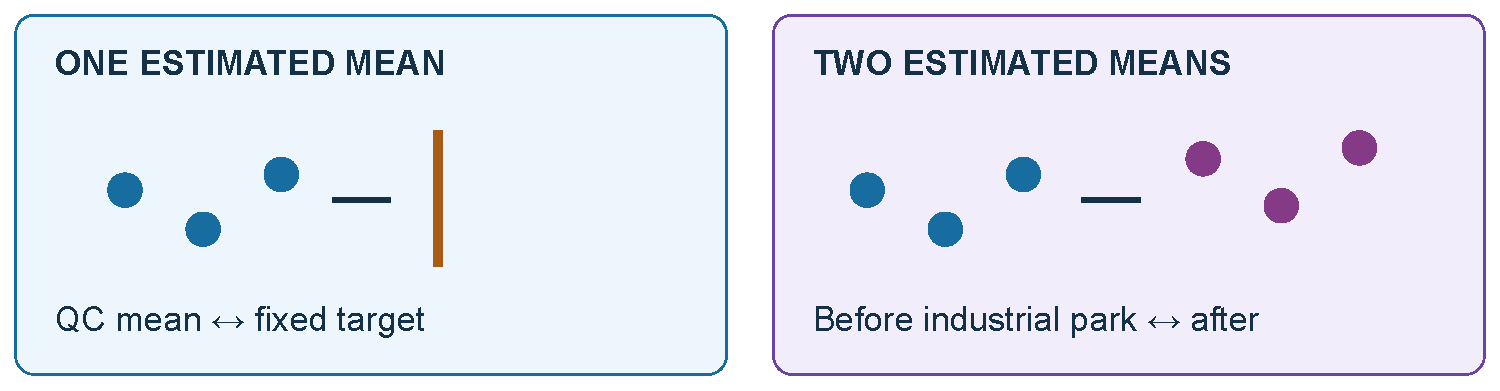
\includegraphics[width=\linewidth,height=.62\textheight,keepaspectratio]{asset-67340acce9581ae7e53572aea06134928f203ecc7800c8406630623d7da8e9ea.pdf}\end{center}

\medskip

\par\medskip
\Needspace{10cm}
\refstepcounter{figure}\label{material-7656a742505cc9060c6dc9938fd63f769f67c2ae904d59b6c0b1376b226ad48b}
\noindent\textbf{Fig.~\ref*{material-7656a742505cc9060c6dc9938fd63f769f67c2ae904d59b6c0b1376b226ad48b}.} One fixed reference or two estimated group means.\par\nopagebreak
\begin{center}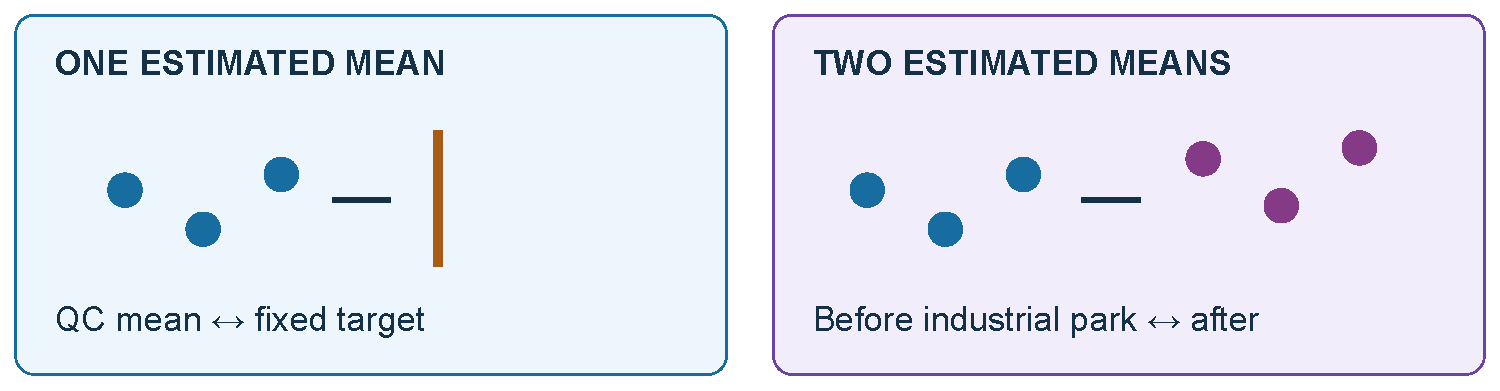
\includegraphics[width=\linewidth,height=.62\textheight,keepaspectratio]{asset-67340acce9581ae7e53572aea06134928f203ecc7800c8406630623d7da8e9ea.pdf}\end{center}

\medskip

\par\medskip
\noindent\begin{minipage}{\linewidth}
\refstepcounter{equation}\label{material-1de4996faf1166371fabce846dbb0e7e45b01fb98fa50240b98d0fe4df2a810c}
\noindent\textbf{Eq.~\ref*{material-1de4996faf1166371fabce846dbb0e7e45b01fb98fa50240b98d0fe4df2a810c}.} One-sample t, SE and residual \ensuremath{\nu} with complete symbols.\par\nopagebreak
\begin{center}\begin{adjustbox}{max width=\linewidth}$\displaystyle t=\frac{\bar x-\mu_0}{s/\sqrt n},\qquad \nu=n-1$\end{adjustbox}\end{center}

\par\noindent\textbf{Symbols}

\begin{itemize}\setlength{\itemsep}{1pt}\setlength{\parsep}{0pt}
\item \textbf{t}: Observed test statistic; dimensionless.
\item \textbf{\ensuremath{\bar{x}}}: Arithmetic sample mean; response unit.
\item \textbf{\ensuremath{\mu}\ensuremath{{}_0}}: Fixed null-reference population mean; same unit.
\item \textbf{s}: Sample SD, using denominator n \ensuremath{-} 1; same unit.
\item \textbf{n}: Number of independent observations; greater than one.
\item \textbf{\ensuremath{\nu} (nu)}: Reference degrees of freedom.
\item \textbf{\ensuremath{\sqrt{\vphantom{x}}}}: Positive square root.
\item \textbf{\ensuremath{-}, /, =}: Subtraction, division and equality.
\end{itemize}

Conditions: independent identically distributed Normal observations, positive variance and fixed reference. Juxtaposition multiplies; subscripts label quantities. Estimated reference uncertainty requires its own model.

\end{minipage}\par
\medskip

The QC experiment \hyperref[material-88a05263accbd8d5fed29d4145364b57b5660a62af7dc6075dc327392b6126e6]{Fig.~\ref*{material-88a05263accbd8d5fed29d4145364b57b5660a62af7dc6075dc327392b6126e6}} starts at target 50 µg/L, sample mean 48.5 µg/L, sample SD 2 µg/L and six independent preparations. It gives t about \ensuremath{-}1.837 and two-sided p about 0.126. Changing mean, SD or independent sample size illustrates hypothetical studies, not permission to edit observations or keep collecting until significance appears. The two-sided question counts both extremes.


\par\medskip
\Needspace{10cm}
\refstepcounter{figure}\label{material-88a05263accbd8d5fed29d4145364b57b5660a62af7dc6075dc327392b6126e6}
\noindent\textbf{Fig.~\ref*{material-88a05263accbd8d5fed29d4145364b57b5660a62af7dc6075dc327392b6126e6}.} QC mean, SD and n explorer with its authored starting state.\par\nopagebreak
\begin{center}
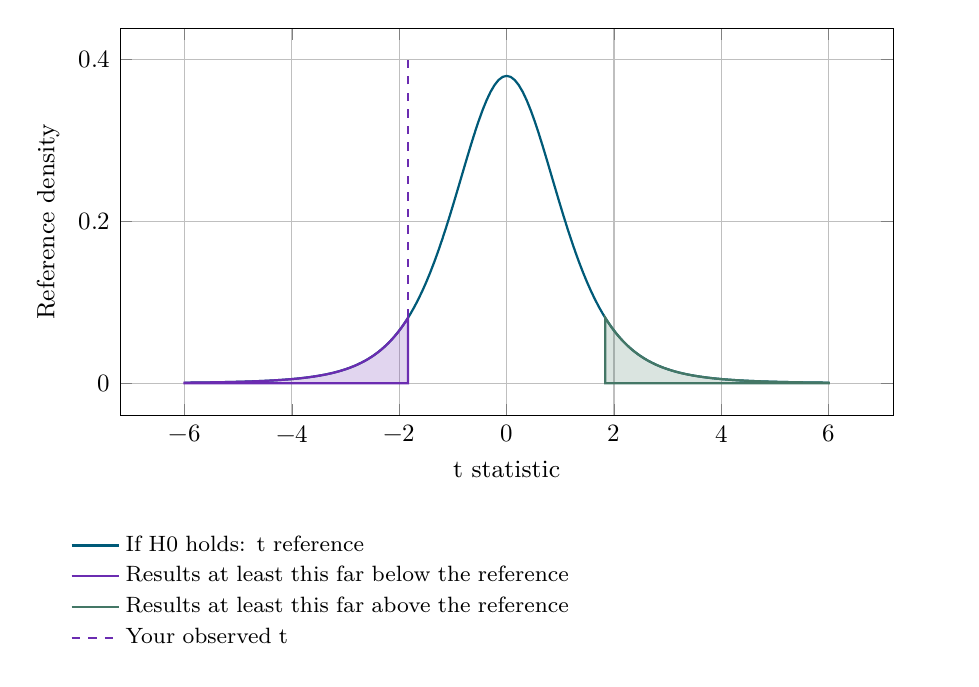
\begin{tikzpicture}
\begin{axis}[width=0.94\linewidth,
height=6.5cm,
scale only axis=false,
grid=major,
tick label style={font=\small},
label style={font=\small},
xlabel={t statistic},
ylabel={Reference density},
legend style={font=\footnotesize,draw=none,at={(0.5,-0.28)},anchor=north,legend columns=1,text width=0.85\linewidth,align=left},
unbounded coords=jump,
scaled ticks=false]
\addplot[color=pcd1,thick,mark=none] coordinates {(-6,0.000688481540137429) (-5.925,0.0007355767679959529) (-5.85,0.0007863901324751119) (-5.775,0.0008412528185500332) (-5.7,0.0009005286807985456) (-5.625,0.0009646177546053254) (-5.55,0.0010339601721534482) (-5.475,0.001109040532433441) (-5.4,0.0011903927806886192) (-5.325,0.0012786056596845242) (-5.25,0.001374328803032794) (-5.175,0.0014782795496180157) (-5.1,0.0015912505680813816) (-5.025,0.0017141183914275325) (-4.95,0.001847852974269337) (-4.875,0.0019935283991452195) (-4.8,0.0021523348738757765) (-4.725,0.002325592179213074) (-4.65,0.0025147647452174794) (-4.575,0.0027214785560028044) (-4.5,0.002947540105833104) (-4.425,0.0031949576551137454) (-4.35,0.003465965062627319) (-4.275,0.0037630485003830624) (-4.2,0.00408897638953717) (-4.125,0.004446832929722545) (-4.05,0.004840055629332371) (-3.975,0.005272477280111668) (-3.9,0.005748372854769392) (-3.825,0.006272511839737553) (-3.75,0.00685021654461358) (-3.675,0.007487426952443685) (-3.6,0.00819077268712905) (-3.525,0.00896765267099772) (-3.45,0.009826323020665953) (-3.375,0.010775993674616737) (-3.3,0.011826934151171158) (-3.225,0.01299058868782331) (-3.15,0.014279700796240562) (-3.075,0.015708446961964793) (-3,0.01729257880022295) (-2.925,0.01904957242093444) (-2.85,0.020998783023804084) (-2.775,0.023161601800264844) (-2.7,0.025561611020544522) (-2.625,0.028224731685617607) (-2.55,0.031179356278633708) (-2.475,0.0344564569147156) (-2.4,0.038089656526431925) (-2.325,0.04211524761635254) (-2.25,0.046572139568152024) (-2.175,0.05150171158843425) (-2.1,0.05694754417217052) (-2.025,0.0629549977542034) (-1.9500000000000002,0.06957060325472626) (-1.875,0.0768412260241492) (-1.7999999999999998,0.08481296289690368) (-1.7249999999999996,0.09352973252936254) (-1.6500000000000004,0.10303152298432797) (-1.5750000000000002,0.11335226887481013) (-1.5,0.124517344646355) (-1.4249999999999998,0.1365406820933797) (-1.3499999999999996,0.14942155007333752) (-1.2750000000000004,0.16314107317460214) (-1.2000000000000002,0.17765861346493533) (-1.125,0.19290819369359277) (-1.0499999999999998,0.20879519794050314) (-0.9749999999999996,0.22519364107025025) (-0.9000000000000004,0.24194434361358957) (-0.8250000000000002,0.2588543741383854) (-0.75,0.2756981160719365) (-0.6749999999999998,0.29222027014680313) (-0.5999999999999996,0.3081410097234197) (-0.5250000000000004,0.32316336196428813) (-0.4500000000000002,0.33698269853401375) (-0.375,0.34929799963442737) (-0.2999999999999998,0.35982432834900946) (-0.22499999999999964,0.36830574912020414) (-0.15000000000000036,0.37452777812642246) (-0.07500000000000018,0.3783283944868038) (0,0.3796066898224941) (0.07500000000000018,0.3783283944868038) (0.15000000000000036,0.37452777812642246) (0.22499999999999964,0.36830574912020414) (0.2999999999999998,0.35982432834900946) (0.375,0.34929799963442737) (0.4500000000000002,0.33698269853401375) (0.5250000000000004,0.32316336196428813) (0.5999999999999996,0.3081410097234197) (0.6749999999999998,0.29222027014680313) (0.75,0.2756981160719365) (0.8250000000000002,0.2588543741383854) (0.9000000000000004,0.24194434361358957) (0.9749999999999996,0.22519364107025025) (1.0499999999999998,0.20879519794050314) (1.125,0.19290819369359277) (1.2000000000000002,0.17765861346493533) (1.2750000000000004,0.16314107317460214) (1.3499999999999996,0.14942155007333752) (1.4249999999999998,0.1365406820933797) (1.5,0.124517344646355) (1.5750000000000002,0.11335226887481013) (1.6500000000000004,0.10303152298432797) (1.7249999999999996,0.09352973252936254) (1.7999999999999998,0.08481296289690368) (1.875,0.0768412260241492) (1.9500000000000002,0.06957060325472626) (2.0250000000000004,0.06295499775420338) (2.0999999999999996,0.056947544172170544) (2.1750000000000007,0.05150171158843419) (2.25,0.046572139568152024) (2.3249999999999993,0.04211524761635256) (2.4000000000000004,0.03808965652643191) (2.4749999999999996,0.03445645691471561) (2.5500000000000007,0.031179356278633653) (2.625,0.028224731685617607) (2.6999999999999993,0.02556161102054457) (2.7750000000000004,0.02316160180026483) (2.8499999999999996,0.02099878302380409) (2.9250000000000007,0.01904957242093441) (3,0.01729257880022295) (3.0749999999999993,0.01570844696196482) (3.1500000000000004,0.014279700796240538) (3.2249999999999996,0.01299058868782331) (3.3000000000000007,0.011826934151171148) (3.375,0.010775993674616737) (3.4499999999999993,0.00982632302066597) (3.5250000000000004,0.00896765267099772) (3.5999999999999996,0.00819077268712905) (3.6750000000000007,0.007487426952443672) (3.75,0.00685021654461358) (3.8249999999999993,0.006272511839737553) (3.9000000000000004,0.005748372854769392) (3.9749999999999996,0.005272477280111668) (4.050000000000001,0.004840055629332371) (4.125,0.004446832929722545) (4.199999999999999,0.004088976389537177) (4.275,0.0037630485003830624) (4.35,0.003465965062627319) (4.425000000000001,0.0031949576551137393) (4.5,0.002947540105833104) (4.574999999999999,0.002721478556002809) (4.65,0.0025147647452174794) (4.725,0.002325592179213074) (4.800000000000001,0.0021523348738757765) (4.875,0.0019935283991452195) (4.949999999999999,0.001847852974269337) (5.025,0.0017141183914275325) (5.1,0.0015912505680813816) (5.175000000000001,0.0014782795496180157) (5.25,0.001374328803032794) (5.324999999999999,0.0012786056596845263) (5.4,0.0011903927806886192) (5.475,0.001109040532433441) (5.550000000000001,0.0010339601721534462) (5.625,0.0009646177546053254) (5.699999999999999,0.0009005286807985456) (5.775,0.0008412528185500332) (5.85,0.0007863901324751119) (5.925000000000001,0.0007355767679959515) (6,0.000688481540137429)};
\addlegendentry{If H0 holds: t reference}
\addplot[color=pcd2,thick,mark=none,fill=pcd2,fill opacity=0.2] coordinates {(-6,0.000688481540137429) (-5.973981983169296,0.0007044174220695071) (-5.947963966338592,0.0007207764272575453) (-5.921945949507888,0.000737571160608412) (-5.895927932677185,0.0007548146408814281) (-5.869909915846481,0.000772520315436701) (-5.843891899015777,0.00079070207554592) (-5.817873882185073,0.000809374272288306) (-5.7918558653543695,0.000828551733055256) (-5.765837848523665,0.0008482497786882685) (-5.739819831692961,0.0008684842412757352) (-5.713801814862258,0.0008892714826352993) (-5.687783798031553,0.0009106284135095147) (-5.66176578120085,0.000932572513503786) (-5.635747764370146,0.0009551218517967694) (-5.6097297475394425,0.000978295108654621) (-5.583711730708738,0.0010021115977818635) (-5.5576937138780345,0.0010265912895429895) (-5.531675697047331,0.0010517548350903539) (-5.505657680216626,0.0010776235914353866) (-5.479639663385923,0.0011042196475017348) (-5.453621646555219,0.0011315658512005453) (-5.427603629724516,0.0011596858375697927) (-5.401585612893811,0.0011886040580213143) (-5.3755675960631075,0.0012183458107410151) (-5.349549579232404,0.0012489372722896935) (-5.3235315624016994,0.0012804055304537982) (-5.297513545570996,0.0013127786183976047) (-5.271495528740292,0.0013460855501703935) (-5.245477511909588,0.001380356357624446) (-5.219459495078884,0.0014156221288020203) (-5.193441478248181,0.0014519150478519154) (-5.167423461417477,0.0014892684365386797) (-5.1414054445867725,0.0015277167974102118) (-5.115387427756069,0.0015672958586921836) (-5.089369410925365,0.0016080426209805797) (-5.063351394094661,0.0016499954058065793) (-5.037333377263957,0.0016931939061509953) (-5.011315360433254,0.0017376792389888437) (-4.98529734360255,0.00178349399994769) (-4.959279326771846,0.001830682320167005) (-4.933261309941142,0.0018792899254492775) (-4.907243293110438,0.0019293641977972838) (-4.881225276279734,0.0019809542394357447) (-4.85520725944903,0.0020341109394196397) (-4.829189242618327,0.002088887042935449) (-4.803171225787622,0.002145337223405917) (-4.777153208956919,0.002203518157513303) (-4.751135192126215,0.0022634886032606907) (-4.725117175295511,0.0023253094811955632) (-4.699099158464808,0.0023890439589247833) (-4.673081141634103,0.002454757539055176) (-4.6470631248034,0.002522518150698945) (-4.621045107972696,0.0025923962446887847) (-4.595027091141992,0.0026644648926527834) (-4.569009074311288,0.0027387998901051017) (-4.5429910574805845,0.0028154798637141966) (-4.51697304064988,0.0028945863829163507) (-4.490955023819176,0.002976204076048475) (-4.464937006988473,0.0030604207511805625) (-4.438918990157768,0.0031473275218344807) (-4.412900973327065,0.0032370189377826557) (-4.386882956496361,0.0033295931211269163) (-4.360864939665657,0.003425151907864573) (-4.334846922834953,0.0035238009951561195) (-4.3088289060042495,0.0036256500945159526) (-4.282810889173546,0.0037308130911548596) (-4.256792872342841,0.003839408209710385) (-4.230774855512138,0.003951558186608774) (-4.204756838681434,0.004067390449309575) (-4.178738821850731,0.00418703730269157) (-4.152720805020026,0.004310636122846409) (-4.126702788189323,0.0044383295585537835) (-4.100684771358619,0.004570265740719496) (-4.0746667545279145,0.004706598500065166) (-4.048648737697211,0.004847487593365917) (-4.022630720866507,0.004993098938539025) (-3.9966127040358033,0.005143604858893985) (-3.9705946872050992,0.005299184336860629) (-3.944576670374395,0.005460023277518702) (-3.9185586535436916,0.00562631478225772) (-3.8925406367129876,0.005798259432901827) (-3.866522619882284,0.005976065586638946) (-3.8405046030515804,0.006159949682097853) (-3.814486586220876,0.006350136556920178) (-3.7884685693901723,0.006546859777176917) (-3.7624505525594687,0.006750361978980811) (-3.7364325357287647,0.006960895222646068) (-3.7104145188980606,0.007178721359746282) (-3.684396502067357,0.007404112413419149) (-3.658378485236653,0.0076373509722626) (-3.6323604684059494,0.007878730598161176) (-3.6063424515752454,0.008128556248374136) (-3.5803244347445413,0.00838714471220622) (-3.5543064179138377,0.008654825062570039) (-3.5282884010831337,0.00893193912273363) (-3.50227038425243,0.00921884194852824) (-3.476252367421726,0.009515902326270127) (-3.450234350591022,0.009823503286624392) (-3.4242163337603184,0.010142042634609674) (-3.398198316929615,0.010471933495908366) (-3.3721803000989103,0.010813604879608557) (-3.3461622832682067,0.011167502257459064) (-3.320144266437503,0.011534088159669713) (-3.294126249606799,0.01191384278723176) (-3.268108232776095,0.012307264640670664) (-3.2420902159453915,0.012714871165072092) (-3.2160721991146874,0.013137199411143236) (-3.190054182283984,0.013574806711983477) (-3.16403616545328,0.014028271375140832) (-3.1380181486225758,0.014498193389423195) (-3.112000131791872,0.014985195145813769) (-3.085982114961168,0.015489922171709686) (-3.0599640981304645,0.01601304387755862) (-3.0339460812997605,0.01655525431481034) (-3.0079280644690565,0.01711727294392819) (-2.981910047638353,0.017699845411016154) (-2.9558920308076493,0.018303744331412925) (-2.929874013976945,0.018929770078380148) (-2.903855997146241,0.01957875157476993) (-2.8778379803155376,0.020251547085294256) (-2.8518199634848336,0.02094904500673386) (-2.8258019466541295,0.021672164653117637) (-2.799783929823426,0.022421857032572892) (-2.7737659129927215,0.023199105612190143) (-2.747747896162018,0.024004927066864162) (-2.7217298793313143,0.024840372007663345) (-2.6957118625006102,0.025706525684840414) (-2.6696938456699066,0.02660450866012995) (-2.6436758288392026,0.027535477442479504) (-2.617657812008499,0.028500625080830386) (-2.5916397951777954,0.02950118170700298) (-2.5656217783470914,0.030538415021144946) (-2.539603761516387,0.03161363071157398) (-2.5135857446856833,0.032728172800184724) (-2.4875677278549793,0.03388342390389592) (-2.4615497110242757,0.035080805401886274) (-2.435531694193572,0.036321777497611105) (-2.409513677362868,0.037607839163802136) (-2.3834956605321644,0.03894052795783764) (-2.3574776437014604,0.04032141969402772) (-2.331459626870756,0.041752127958494895) (-2.3054416100400523,0.04323430345144665) (-2.2794235932093487,0.044769633140740485) (-2.2534055763786447,0.04635983920973403) (-2.227387559547941,0.048006677781507086) (-2.201369542717237,0.04971193740064018) (-2.1753515258865335,0.051477437252845676) (-2.14933350905583,0.053305025101887296) (-2.123315492225126,0.055196574922395894) (-2.0972974753944214,0.05715398420641402) (-2.0712794585637178,0.059179170920788476) (-2.0452614417330137,0.06127407009189884) (-2.01924342490231,0.06344062999367324) (-1.9932254080716065,0.0656808079144311) (-1.967207391240903,0.0679965654778117) (-1.9411893744101985,0.07038986349293891) (-1.9151713575794949,0.07286265630904526) (-1.8891533407487904,0.07541688565007428) (-1.8631353239180868,0.07805447390531443) (-1.8371173070873832,0.08077731685293615)} \closedcycle;
\addlegendentry{Results at least this far below the reference}
\addplot[color=pcd3,thick,mark=none,fill=pcd3,fill opacity=0.2] coordinates {(1.8371173070873834,0.08077731685293611) (1.8631353239180872,0.07805447390531439) (1.889153340748791,0.07541688565007418) (1.9151713575794949,0.07286265630904526) (1.941189374410199,0.07038986349293888) (1.9672073912409027,0.06799656547781173) (1.9932254080716065,0.0656808079144311) (2.0192434249023106,0.06344062999367321) (2.045261441733014,0.06127407009189879) (2.071279458563718,0.059179170920788456) (2.097297475394422,0.057153984206413974) (2.123315492225126,0.055196574922395894) (2.14933350905583,0.053305025101887296) (2.1753515258865335,0.051477437252845676) (2.2013695427172375,0.04971193740064013) (2.227387559547941,0.048006677781507086) (2.253405576378645,0.04635983920973399) (2.2794235932093487,0.044769633140740485) (2.3054416100400528,0.04323430345144663) (2.331459626870757,0.04175212795849484) (2.3574776437014604,0.04032141969402772) (2.3834956605321644,0.03894052795783764) (2.4095136773628685,0.037607839163802115) (2.435531694193572,0.036321777497611105) (2.4615497110242757,0.035080805401886274) (2.4875677278549797,0.033883423903895905) (2.5135857446856837,0.032728172800184696) (2.5396037615163873,0.03161363071157396) (2.5656217783470914,0.030538415021144946) (2.5916397951777954,0.02950118170700298) (2.617657812008499,0.028500625080830386) (2.643675828839203,0.02753547744247948) (2.6696938456699066,0.02660450866012995) (2.6957118625006107,0.02570652568484039) (2.7217298793313143,0.024840372007663345) (2.7477478961620183,0.02400492706686414) (2.7737659129927223,0.023199105612190116) (2.799783929823426,0.022421857032572892) (2.82580194665413,0.021672164653117627) (2.851819963484834,0.020949045006733842) (2.8778379803155376,0.020251547085294256) (2.903855997146241,0.01957875157476993) (2.9298740139769457,0.018929770078380124) (2.9558920308076493,0.018303744331412925) (2.981910047638353,0.017699845411016154) (3.007928064469057,0.01711727294392819) (3.033946081299761,0.01655525431481034) (3.0599640981304645,0.01601304387755862) (3.085982114961168,0.015489922171709686) (3.1120001317918726,0.014985195145813741) (3.138018148622576,0.014498193389423195) (3.16403616545328,0.014028271375140832) (3.190054182283984,0.013574806711983477) (3.216072199114688,0.013137199411143236) (3.2420902159453915,0.012714871165072092) (3.2681082327760955,0.012307264640670643) (3.2941262496067996,0.011913842787231739) (3.320144266437503,0.011534088159669713) (3.3461622832682067,0.011167502257459064) (3.3721803000989112,0.010813604879608538) (3.398198316929615,0.010471933495908366) (3.4242163337603184,0.010142042634609674) (3.450234350591023,0.009823503286624392) (3.4762523674217265,0.009515902326270118) (3.50227038425243,0.00921884194852824) (3.5282884010831337,0.00893193912273363) (3.5543064179138377,0.008654825062570039) (3.5803244347445418,0.00838714471220622) (3.6063424515752454,0.008128556248374136) (3.6323604684059494,0.007878730598161176) (3.6583784852366534,0.0076373509722626) (3.684396502067357,0.007404112413419149) (3.710414518898061,0.007178721359746269) (3.736432535728765,0.006960895222646055) (3.7624505525594687,0.006750361978980811) (3.7884685693901727,0.006546859777176905) (3.8144865862208768,0.006350136556920178) (3.8405046030515804,0.006159949682097853) (3.866522619882284,0.005976065586638946) (3.8925406367129884,0.005798259432901817) (3.918558653543692,0.00562631478225772) (3.9445766703743956,0.005460023277518702) (3.9705946872050992,0.005299184336860629) (3.996612704035803,0.005143604858893985) (4.022630720866507,0.004993098938539025) (4.048648737697211,0.004847487593365917) (4.0746667545279145,0.004706598500065166) (4.100684771358619,0.004570265740719496) (4.126702788189323,0.0044383295585537835) (4.152720805020026,0.004310636122846409) (4.178738821850731,0.00418703730269157) (4.204756838681434,0.004067390449309575) (4.230774855512138,0.003951558186608774) (4.256792872342842,0.003839408209710378) (4.282810889173546,0.0037308130911548596) (4.3088289060042495,0.0036256500945159526) (4.334846922834953,0.0035238009951561195) (4.360864939665658,0.003425151907864573) (4.386882956496361,0.0033295931211269163) (4.412900973327065,0.0032370189377826557) (4.438918990157768,0.0031473275218344807) (4.464937006988473,0.0030604207511805625) (4.490955023819176,0.002976204076048475) (4.51697304064988,0.0028945863829163507) (4.5429910574805845,0.0028154798637141966) (4.569009074311288,0.0027387998901051017) (4.595027091141992,0.0026644648926527834) (4.621045107972696,0.0025923962446887847) (4.6470631248034,0.002522518150698945) (4.673081141634103,0.002454757539055176) (4.699099158464808,0.0023890439589247833) (4.7251171752955115,0.002325309481195559) (4.751135192126215,0.0022634886032606907) (4.777153208956919,0.002203518157513303) (4.803171225787623,0.002145337223405917) (4.829189242618327,0.002088887042935449) (4.85520725944903,0.0020341109394196397) (4.881225276279734,0.0019809542394357447) (4.907243293110438,0.0019293641977972838) (4.933261309941142,0.0018792899254492775) (4.959279326771846,0.001830682320167005) (4.98529734360255,0.00178349399994769) (5.011315360433254,0.0017376792389888437) (5.037333377263957,0.0016931939061509953) (5.063351394094662,0.0016499954058065793) (5.089369410925365,0.0016080426209805797) (5.115387427756069,0.0015672958586921836) (5.141405444586773,0.0015277167974102118) (5.167423461417477,0.0014892684365386797) (5.193441478248181,0.0014519150478519154) (5.219459495078884,0.0014156221288020203) (5.245477511909588,0.001380356357624446) (5.271495528740292,0.0013460855501703935) (5.297513545570997,0.0013127786183976047) (5.3235315624017,0.0012804055304537958) (5.349549579232404,0.0012489372722896935) (5.3755675960631075,0.0012183458107410151) (5.401585612893811,0.0011886040580213143) (5.427603629724516,0.0011596858375697927) (5.453621646555219,0.0011315658512005453) (5.479639663385923,0.0011042196475017348) (5.505657680216627,0.0010776235914353866) (5.531675697047331,0.0010517548350903539) (5.5576937138780345,0.0010265912895429895) (5.583711730708739,0.0010021115977818617) (5.6097297475394425,0.000978295108654621) (5.635747764370146,0.0009551218517967694) (5.66176578120085,0.000932572513503786) (5.687783798031553,0.0009106284135095147) (5.713801814862258,0.0008892714826352993) (5.739819831692962,0.0008684842412757352) (5.765837848523666,0.0008482497786882655) (5.7918558653543695,0.000828551733055256) (5.817873882185073,0.000809374272288306) (5.843891899015777,0.00079070207554592) (5.86990991584648,0.000772520315436701) (5.895927932677185,0.0007548146408814281) (5.921945949507888,0.000737571160608412) (5.947963966338593,0.0007207764272575453) (5.973981983169296,0.0007044174220695071) (6,0.000688481540137429)} \closedcycle;
\addlegendentry{Results at least this far above the reference}
\addplot[color=pcd2,dashed,thick] coordinates {(-1.8371173070873834,0) (-1.8371173070873834,0.39858702431361887)};
\addlegendentry{Your observed t}
\end{axis}
\end{tikzpicture}
\end{center}

% Full-precision experiment details: {"blockId":"ex:l6-i11bc--block","parameters":[{"key":"mean","label":"Sample mean (µg/L)","value":48.5},{"key":"sd","label":"Sample SD (µg/L)","value":2},{"key":"n","label":"Independent preparations n","value":6},{"key":"view","label":"Observed t view","value":0},{"key":"reference","label":"Fixed QC target (µg/L)","value":50},{"key":"alpha","label":"Chosen alpha","value":0.05},{"key":"direction","label":"Two-sided question","value":0},{"key":"effect","label":"Unused alternative departure","value":0},{"key":"M","label":"Studies in simulation view","value":4000},{"key":"seed","label":"Reproducible seed","value":617}],"readouts":[{"label":"Observed t","value":-1.8371173070873834},{"label":"ν","value":5},{"label":"p-value","value":0.1256124312189737},{"label":"Reject H0 at chosen alpha?","value":"No"}],"note":"Move the sample mean, sample SD or independent sample size. Shaded tails count results at least as extreme as yours, assuming the null reference. Compare the full calculated p-value with the chosen alpha; the drawing shows a finite part of the tails.","markers":[[{"x":-1.8371173070873834,"label":"Your observed t"}]]}

\medskip

The separate recovery example \hyperref[material-fd86e8304c9a50afc12bf7efac33315633432944fffe642415ffc8fa8521d12c]{Fig.~\ref*{material-fd86e8304c9a50afc12bf7efac33315633432944fffe642415ffc8fa8521d12c}} asks whether a minimum population mean recovery of 80\% is exceeded. \textbf{H\ensuremath{{}_0}: \ensuremath{\mu} \ensuremath{\le} 80\%; H\ensuremath{{}_1}: \ensuremath{\mu} > 80\%}. The six synthetic values average \textbf{81.5\%}. The R-style mimic \hyperref[material-11ae66795f86539682589f0b311cfe0e5993c724bdfc6e6d370d0164cd5c9de4]{Table~\ref*{material-11ae66795f86539682589f0b311cfe0e5993c724bdfc6e6d370d0164cd5c9de4}} reports \textbf{t = 3.5032, \ensuremath{\nu} = 5, upper-tail p = 0.008612}. Rejection at 5\% supports the population mean being above the illustrative minimum. Individual preparations still vary around that mean. Further reading: NIST one-sample t-test \hyperref[material-89b243493ab2e38f1da886da7ef954857447a356a48f901b2b4008e6538f5eb2]{Fig.~\ref*{material-89b243493ab2e38f1da886da7ef954857447a356a48f901b2b4008e6538f5eb2}} and t reference table \hyperref[material-454ec396cc8632a77cbe3c3660b108fde536dac517527502b24966cf36fbdec1]{Fig.~\ref*{material-454ec396cc8632a77cbe3c3660b108fde536dac517527502b24966cf36fbdec1}}.


\par\medskip
\Needspace{10cm}
\refstepcounter{figure}\label{material-fd86e8304c9a50afc12bf7efac33315633432944fffe642415ffc8fa8521d12c}
\noindent\textbf{Fig.~\ref*{material-fd86e8304c9a50afc12bf7efac33315633432944fffe642415ffc8fa8521d12c}.} Six synthetic recovery preparations, including separate repeated values.\par\nopagebreak
\begin{center}
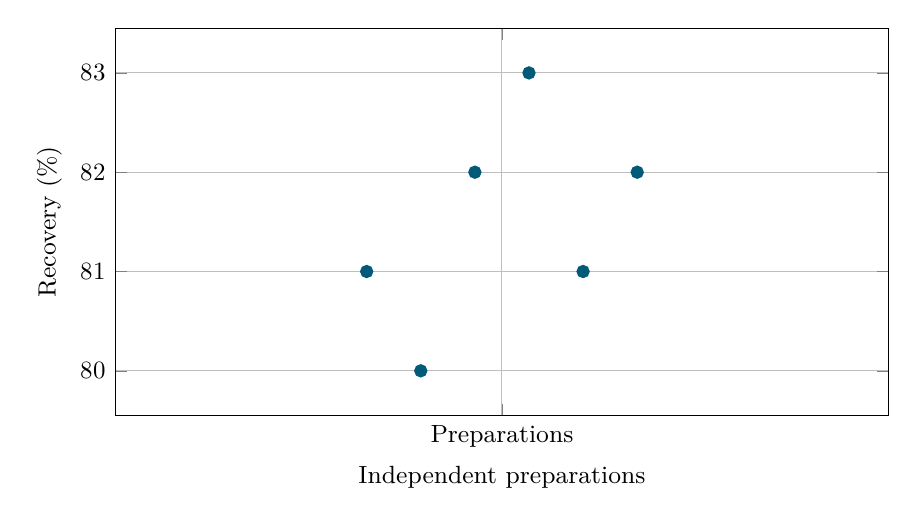
\begin{tikzpicture}
\begin{axis}[width=0.94\linewidth,
height=6.5cm,
scale only axis=false,
grid=major,
tick label style={font=\small},
label style={font=\small},
xlabel={Independent preparations},
ylabel={Recovery (\%)},
legend style={font=\footnotesize,draw=none,at={(0.5,-0.28)},anchor=north,legend columns=1,text width=0.85\linewidth,align=left},
unbounded coords=jump,
scaled ticks=false,
ymin=79.55,
ymax=83.45,
xmin=0.5,
xmax=1.5,
xtick={1},
xticklabels={{Preparations}}]
\addplot[color=pcd1,thick,only marks,mark=*] coordinates {(0.825,81) (0.895,80) (0.965,82) (1.035,83) (1.105,81) (1.175,82)};

\end{axis}
\end{tikzpicture}
\end{center}


\medskip

\par\medskip
\Needspace{8\baselineskip}
\refstepcounter{scripttable}\label{material-11ae66795f86539682589f0b311cfe0e5993c724bdfc6e6d370d0164cd5c9de4}
\noindent\textbf{Table~\ref*{material-11ae66795f86539682589f0b311cfe0e5993c724bdfc6e6d370d0164cd5c9de4}.} R-style one-sided recovery report; authored mimic, not claimed live output.\par\nopagebreak
\begin{longtable}{@{}p{\dimexpr0.500000\linewidth-2\tabcolsep\relax}p{\dimexpr0.500000\linewidth-2\tabcolsep\relax}@{}}
Field & Result \\ \hline
\endhead
Hypotheses & H\ensuremath{{}_0}: mean at or below 80\%; H\ensuremath{{}_1}: above 80\% \\ \hline
Statistic / \ensuremath{\nu} & t = 3.5032; \ensuremath{\nu} = 5 \\ \hline
p-value & 0.008612 \ensuremath{\cdot} upper t tail \\ \hline
Sample estimate & Mean 81.5\%; n = 6; SD 1.049 percentage points \\ \hline
Reference & Upper t tail at the 80\% null boundary \\ \hline
Decision at 5\% & Reject H\ensuremath{{}_0} under independent Normal preparations: evidence for a population mean above 80\%. Individual preparations vary. \\ \hline
\end{longtable}
\medskip

\par\medskip
\Needspace{10cm}
\refstepcounter{figure}\label{material-89b243493ab2e38f1da886da7ef954857447a356a48f901b2b4008e6538f5eb2}
\noindent\textbf{Fig.~\ref*{material-89b243493ab2e38f1da886da7ef954857447a356a48f901b2b4008e6538f5eb2}.} NIST: one-sample t reference.\par\nopagebreak
\noindent\href{https://www.itl.nist.gov/div898/handbook/eda/section3/eda352.htm}{NIST: one-sample t-test}\par
\nolinkurl{https://www.itl.nist.gov/div898/handbook/eda/section3/eda352.htm}\par

\medskip

\par\medskip
\Needspace{10cm}
\refstepcounter{figure}\label{material-454ec396cc8632a77cbe3c3660b108fde536dac517527502b24966cf36fbdec1}
\noindent\textbf{Fig.~\ref*{material-454ec396cc8632a77cbe3c3660b108fde536dac517527502b24966cf36fbdec1}.} NIST: Student t critical values.\par\nopagebreak
\noindent\href{https://www.itl.nist.gov/div898/handbook/eda/section3/eda3672.htm}{NIST: t reference table}\par
\nolinkurl{https://www.itl.nist.gov/div898/handbook/eda/section3/eda3672.htm}\par

\medskip

\clearpage
\section{Independent groups, shared variance and real pairs}
Sampling identity comes before software choice. The structures in \hyperref[material-c6165c9700b01ef31032f9ef6753087a49d9f742b06ad6cca09a76406bb9b7d1]{Fig.~\ref*{material-c6165c9700b01ef31032f9ef6753087a49d9f742b06ad6cca09a76406bb9b7d1}} distinguish independent groups from matched pairs. For independent Normal samples with a justified common variance, the pooled construction \hyperref[material-fcdd0f74a575bed3c21eef981a2409870a0e9b7c8a892fc137b18f042b4a649a]{Eq.~\ref*{material-fcdd0f74a575bed3c21eef981a2409870a0e9b7c8a892fc137b18f042b4a649a}} combines sample variances using \textbf{residual degrees of freedom as weights}. The river drawing \hyperref[material-b813da46780b31c64ab6cb4f96ec3c1b2c5769771baa458003201cc98b330ec3]{Fig.~\ref*{material-b813da46780b31c64ab6cb4f96ec3c1b2c5769771baa458003201cc98b330ec3}} represents separate upstream and downstream sites. Prior method validation and a homogeneous matrix could support similar within-region measurement variance. Another plausible setting is two randomized groups measured by the same validated assay.


\par\medskip
\Needspace{10cm}
\refstepcounter{figure}\label{material-c6165c9700b01ef31032f9ef6753087a49d9f742b06ad6cca09a76406bb9b7d1}
\noindent\textbf{Fig.~\ref*{material-c6165c9700b01ef31032f9ef6753087a49d9f742b06ad6cca09a76406bb9b7d1}.} Fixed target, separate units and matched identities.\par\nopagebreak
\begin{center}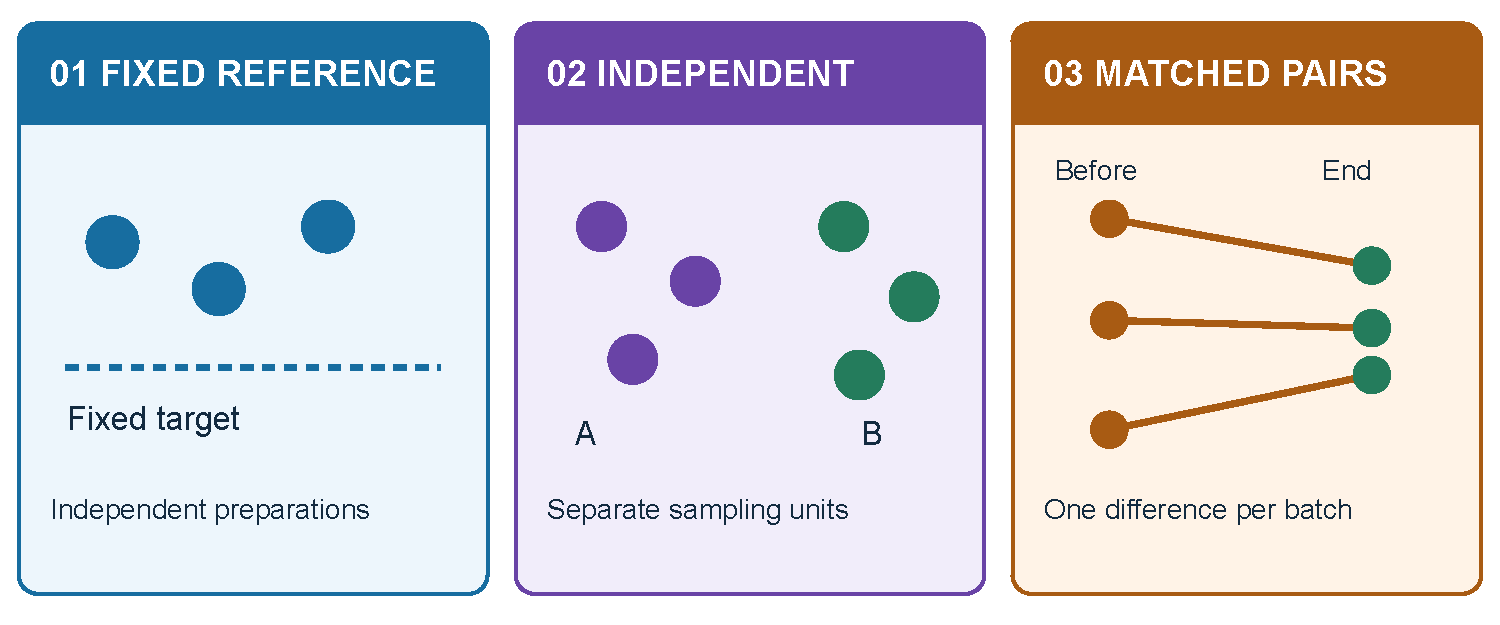
\includegraphics[width=\linewidth,height=.62\textheight,keepaspectratio]{asset-c1e3c5dedf8fc945a8f97510e594bd0a16d963060275133fdbc1a2f80bd87af4.pdf}\end{center}

\medskip

\par\medskip
\noindent\begin{minipage}{\linewidth}
\refstepcounter{equation}\label{material-fcdd0f74a575bed3c21eef981a2409870a0e9b7c8a892fc137b18f042b4a649a}
\noindent\textbf{Eq.~\ref*{material-fcdd0f74a575bed3c21eef981a2409870a0e9b7c8a892fc137b18f042b4a649a}.} Pooled variance weighted by residual degrees of freedom.\par\nopagebreak
\begin{center}\begin{adjustbox}{max width=\linewidth}$\displaystyle \begin{gathered}\underbrace{s_p^2}_{\text{weighted variance}}=\frac{(n_1-1)s_1^2+(n_2-1)s_2^2}{n_1+n_2-2}\\t=\frac{\bar x_1-\bar x_2-\Delta_0}{s_p\sqrt{1/n_1+1/n_2}}\\\nu=n_1+n_2-2\end{gathered}$\end{adjustbox}\end{center}

\par\noindent\textbf{Symbols}

\begin{itemize}\setlength{\itemsep}{1pt}\setlength{\parsep}{0pt}
\item \textbf{1, 2}: Independent-group indices.
\item \textbf{n\ensuremath{{}_1}, n\ensuremath{{}_2}}: Group sample sizes, each greater than one.
\item \textbf{\ensuremath{\bar{x}}\ensuremath{{}_1}, \ensuremath{\bar{x}}\ensuremath{{}_2}}: Group means; response unit.
\item \textbf{s\ensuremath{{}_1}\ensuremath{{}^2}, s\ensuremath{{}_2}\ensuremath{{}^2}}: Sample variances, denominators n\ensuremath{{}_1} \ensuremath{-} 1 and n\ensuremath{{}_2} \ensuremath{-} 1; squared response unit.
\item \textbf{s\ensuremath{{}_p}\ensuremath{{}^2}}: Pooled variance weighted by residual degrees of freedom; p labels pooling.
\item \textbf{s\ensuremath{{}_p}}: Positive square root of pooled variance; response unit.
\item \textbf{Δ\ensuremath{{}_0}}: Null population mean difference, often zero; response unit.
\item \textbf{t; \ensuremath{\nu}}: Dimensionless test statistic; residual degrees of freedom.
\item \textbf{2; \ensuremath{\sqrt{\vphantom{x}}}}: Squaring; positive square root.
\item \textbf{+, \ensuremath{-}, =, fraction bars}: Add, subtract, equal, divide.
\end{itemize}

Conditions: independent Normal samples with one common positive population variance. Juxtaposition multiplies; parentheses group. The underbrace labels the weighted variance.

\end{minipage}\par
\medskip

\par\medskip
\Needspace{10cm}
\refstepcounter{figure}\label{material-b813da46780b31c64ab6cb4f96ec3c1b2c5769771baa458003201cc98b330ec3}
\noindent\textbf{Fig.~\ref*{material-b813da46780b31c64ab6cb4f96ec3c1b2c5769771baa458003201cc98b330ec3}.} Independent upstream/downstream sampling around an industrial park.\par\nopagebreak
\begin{center}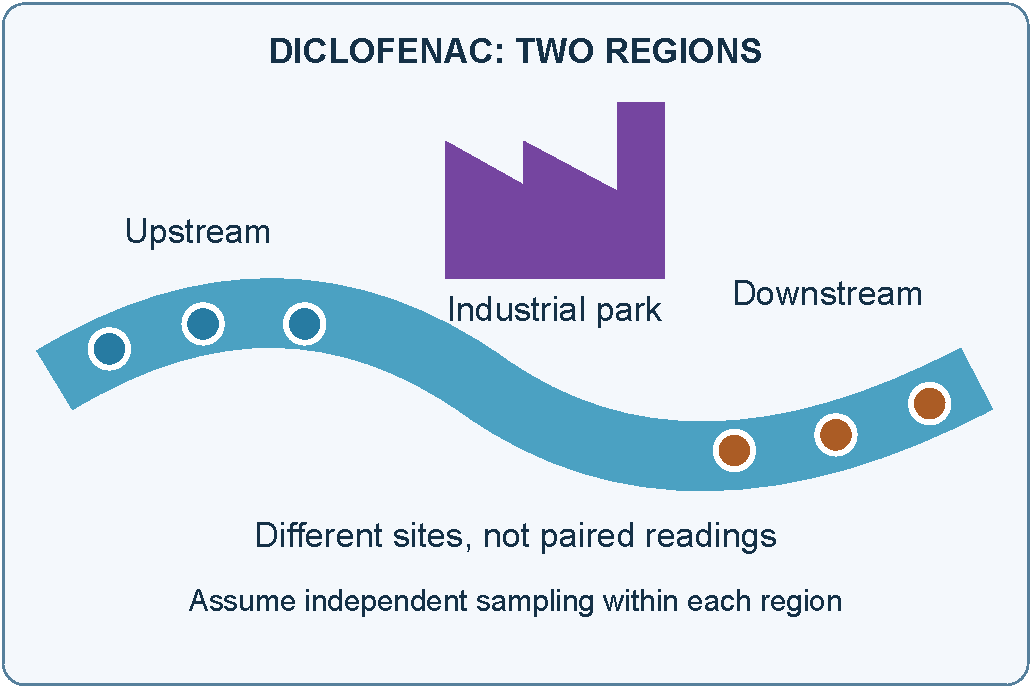
\includegraphics[width=\linewidth,height=.62\textheight,keepaspectratio]{asset-c759afbdaa9a6a1f8f522e3f66542f0ee3b239ef2c79faf88e21eb146b944427.pdf}\end{center}

\medskip

An oxidation batch has a different structure. The before/end bottles in \hyperref[material-6930f7102301e4ce9de868d2da55c6dc66032f520d5fe7efd616f55db9e59fc7]{Fig.~\ref*{material-6930f7102301e4ce9de868d2da55c6dc66032f520d5fe7efd616f55db9e59fc7}} share a batch, so keep that identity and form one \textbf{difference} per independent batch using \hyperref[material-cd3d782c9d2eeb959af659280c9e14187707b1d58e39c2a6cf643e35a73a0efe]{Eq.~\ref*{material-cd3d782c9d2eeb959af659280c9e14187707b1d58e39c2a6cf643e35a73a0efe}}. Exact paired-t inference assumes independent Normal differences. The six differences in \hyperref[material-86397ba56fc8564506e95d8b3665530913a5f3cd7e57a9110413b075a78da0d0]{Fig.~\ref*{material-86397ba56fc8564506e95d8b3665530913a5f3cd7e57a9110413b075a78da0d0}} include zero and average \textbf{2.833 mg/L}. The report \hyperref[material-b6c0280b5f2172c48b46e488643fee349814d577744a3dffc1c42b58a80e6ef0]{Table~\ref*{material-b6c0280b5f2172c48b46e488643fee349814d577744a3dffc1c42b58a80e6ef0}} gives \textbf{t = 4.0294, \ensuremath{\nu} = 5, two-sided p = 0.01003}. All batches remain; the conclusion concerns the population mean before-minus-end decrease. Time-related competing explanations still matter for causal attribution.


\par\medskip
\noindent\begin{minipage}{\linewidth}
\refstepcounter{equation}\label{material-cd3d782c9d2eeb959af659280c9e14187707b1d58e39c2a6cf643e35a73a0efe}
\noindent\textbf{Eq.~\ref*{material-cd3d782c9d2eeb959af659280c9e14187707b1d58e39c2a6cf643e35a73a0efe}.} Form original batch differences before calculating a one-sample t statistic.\par\nopagebreak
\begin{center}\begin{adjustbox}{max width=\linewidth}$\displaystyle d_i=x_i-y_i,\quad t=\frac{\bar d-\Delta_0}{s_d/\sqrt n},\quad \nu=n-1$\end{adjustbox}\end{center}

\par\noindent\textbf{Symbols}

\begin{itemize}\setlength{\itemsep}{1pt}\setlength{\parsep}{0pt}
\item \textbf{i}: Original matched batch index.
\item \textbf{x\ensuremath{{}_i}, y\ensuremath{{}_i}}: Before and end concentration in that same batch; mg/L.
\item \textbf{d\ensuremath{{}_i}; \ensuremath{\bar{d}}}: Before-minus-end difference; mean of differences; mg/L.
\item \textbf{s\_d}: Sample SD of differences, denominator n \ensuremath{-} 1; mg/L.
\item \textbf{Δ\ensuremath{{}_0}}: Null mean difference, here zero; mg/L.
\item \textbf{n}: Independent batches, not individual readings; greater than one.
\item \textbf{t; \ensuremath{\nu}}: Dimensionless statistic; reference degrees of freedom.
\item \textbf{\ensuremath{\sqrt{\vphantom{x}}}; \ensuremath{-}; =; fraction bars}: Positive square root, subtract, equal, divide.
\end{itemize}

Conditions: independent Normal batch differences with positive variance. Original readings within a batch may be dependent; do not sort them to create new pairs. Subscripts label quantities; parentheses group.

\end{minipage}\par
\medskip

\par\medskip
\Needspace{10cm}
\refstepcounter{figure}\label{material-6930f7102301e4ce9de868d2da55c6dc66032f520d5fe7efd616f55db9e59fc7}
\noindent\textbf{Fig.~\ref*{material-6930f7102301e4ce9de868d2da55c6dc66032f520d5fe7efd616f55db9e59fc7}.} Before/end samples from one stirred oxidation batch are dependent.\par\nopagebreak
\begin{center}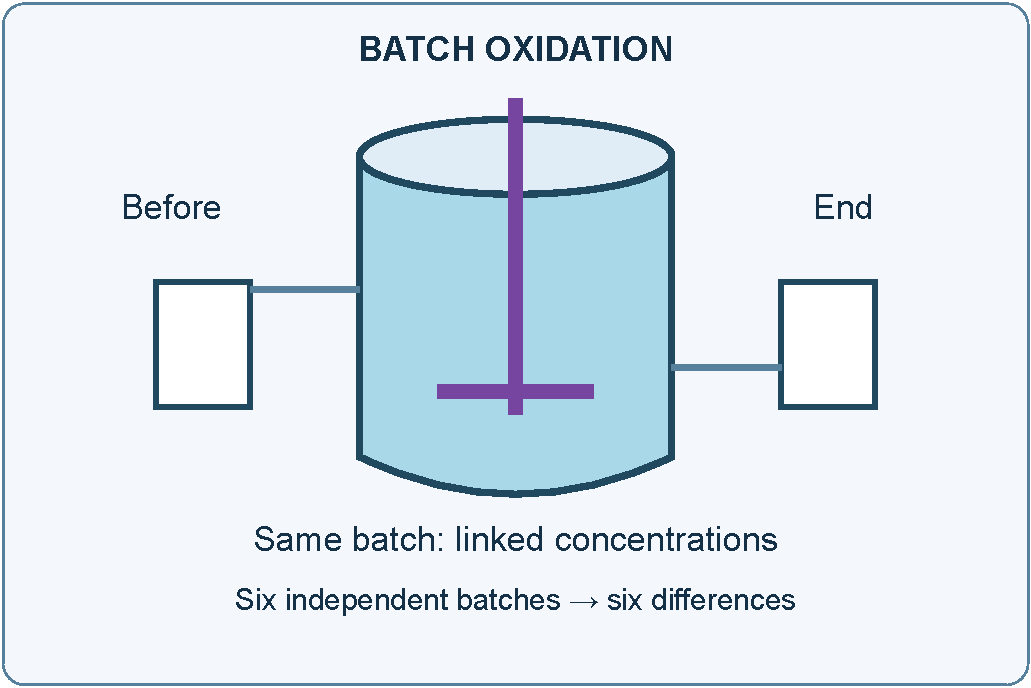
\includegraphics[width=\linewidth,height=.62\textheight,keepaspectratio]{asset-079a89a76dffb380e445b8c7d7cc68a23e7f257aaba67989da14fd4b12279c7f.pdf}\end{center}

\medskip

\par\medskip
\Needspace{10cm}
\refstepcounter{figure}\label{material-86397ba56fc8564506e95d8b3665530913a5f3cd7e57a9110413b075a78da0d0}
\noindent\textbf{Fig.~\ref*{material-86397ba56fc8564506e95d8b3665530913a5f3cd7e57a9110413b075a78da0d0}.} Independent synthetic batch differences, including no observed change.\par\nopagebreak
\begin{center}
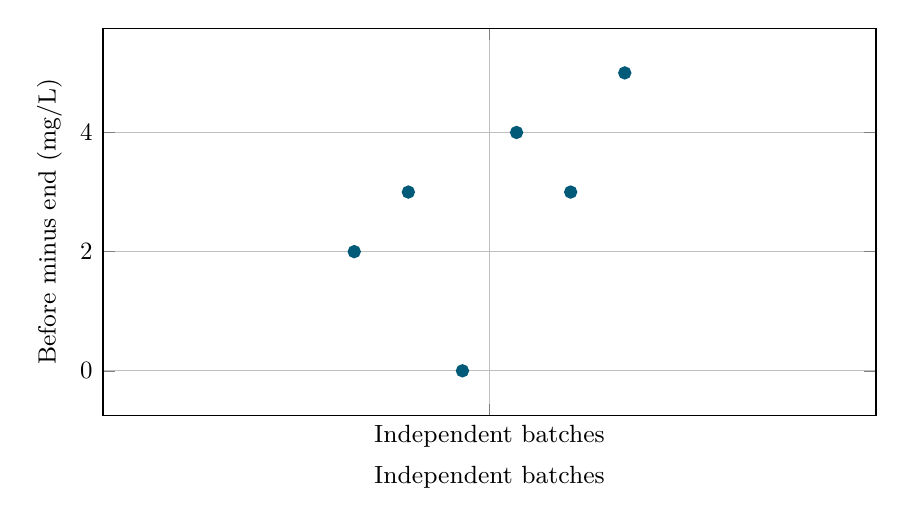
\begin{tikzpicture}
\begin{axis}[width=0.94\linewidth,
height=6.5cm,
scale only axis=false,
grid=major,
tick label style={font=\small},
label style={font=\small},
xlabel={Independent batches},
ylabel={Before minus end (mg/L)},
legend style={font=\footnotesize,draw=none,at={(0.5,-0.28)},anchor=north,legend columns=1,text width=0.85\linewidth,align=left},
unbounded coords=jump,
scaled ticks=false,
ymin=-0.75,
ymax=5.75,
xmin=0.5,
xmax=1.5,
xtick={1},
xticklabels={{Independent batches}}]
\addplot[color=pcd1,thick,only marks,mark=*] coordinates {(0.825,2) (0.895,3) (0.965,0) (1.035,4) (1.105,3) (1.175,5)};

\end{axis}
\end{tikzpicture}
\end{center}


\medskip

\par\medskip
\Needspace{8\baselineskip}
\refstepcounter{scripttable}\label{material-b6c0280b5f2172c48b46e488643fee349814d577744a3dffc1c42b58a80e6ef0}
\noindent\textbf{Table~\ref*{material-b6c0280b5f2172c48b46e488643fee349814d577744a3dffc1c42b58a80e6ef0}.} Paired-t R-style report with the native-unit mean difference.\par\nopagebreak
\begin{longtable}{@{}p{\dimexpr0.500000\linewidth-2\tabcolsep\relax}p{\dimexpr0.500000\linewidth-2\tabcolsep\relax}@{}}
Field & Result \\ \hline
\endhead
Alternative & H\ensuremath{{}_0}: zero population mean change; H\ensuremath{{}_1}: nonzero \\ \hline
Statistic / \ensuremath{\nu} / p & t = 4.0294; \ensuremath{\nu} = 5; two-sided p = 0.01003 \\ \hline
Mean difference & Before minus end: 2.833 mg/L; six batches \\ \hline
Reference & Two t tails under zero population mean difference \\ \hline
Decision / model & Reject at 5\%; independent Normal batch differences. Mean concentration falls; control time-related alternatives before claiming causality. \\ \hline
\end{longtable}
\medskip

Welch's construction \hyperref[material-617b0c3f5529272069c1b0a3452ab6d012a7a81bb5dc10a3cca21b881af2ec9c]{Eq.~\ref*{material-617b0c3f5529272069c1b0a3452ab6d012a7a81bb5dc10a3cca21b881af2ec9c}} retains each group's own variance estimate and calibrates an approximate, generally fractional \textbf{\ensuremath{\nu}}. The independent sets in \hyperref[material-ce1cbd732119479a3764d2c581195ae9219179d7288fda899398511c82c8f56f]{Fig.~\ref*{material-ce1cbd732119479a3764d2c581195ae9219179d7288fda899398511c82c8f56f}} comprise five NIR and six HPLC-MS preparations from one homogeneous reference material. Shared samples measured twice would require pairing. The dot plot \hyperref[material-b4ea53f64452a50d49c4741496838ca77459fe1afebbc902f30b28e0942186de]{Fig.~\ref*{material-b4ea53f64452a50d49c4741496838ca77459fe1afebbc902f30b28e0942186de}} has means \textbf{10 and 15 µg/L}. In \hyperref[material-208e0fd84411d4dcfede0de78aa9bfa57e6d79e60db66e2647ab1eed0a22c302]{Table~\ref*{material-208e0fd84411d4dcfede0de78aa9bfa57e6d79e60db66e2647ab1eed0a22c302}}, NIR minus HPLC-MS is \textbf{\ensuremath{-}5 µg/L}, with \textbf{\ensuremath{\nu} \ensuremath{\approx} 6.972, p \ensuremath{\approx} 0.02089}. Accuracy and method agreement require their own validation. NIST compares the three t constructions in \hyperref[material-c75d95ca59c1d780eb96008b60ae04bc4671cf6f23aa115926e8043b71c83071]{Fig.~\ref*{material-c75d95ca59c1d780eb96008b60ae04bc4671cf6f23aa115926e8043b71c83071}}.


\par\medskip
\noindent\begin{minipage}{\linewidth}
\refstepcounter{equation}\label{material-617b0c3f5529272069c1b0a3452ab6d012a7a81bb5dc10a3cca21b881af2ec9c}
\noindent\textbf{Eq.~\ref*{material-617b0c3f5529272069c1b0a3452ab6d012a7a81bb5dc10a3cca21b881af2ec9c}.} Separate mean-variance contributions and approximate Welch \ensuremath{\nu}.\par\nopagebreak
\begin{center}\begin{adjustbox}{max width=\linewidth}$\displaystyle \begin{gathered}v_j=\frac{s_j^2}{n_j},\quad t=\frac{\bar x_1-\bar x_2-\Delta_0}{\sqrt{v_1+v_2}}\\\nu=\frac{(v_1+v_2)^2}{v_1^2/(n_1-1)+v_2^2/(n_2-1)}\end{gathered}$\end{adjustbox}\end{center}

\par\noindent\textbf{Symbols}

\begin{itemize}\setlength{\itemsep}{1pt}\setlength{\parsep}{0pt}
\item \textbf{j; 1, 2}: System index; NIR and HPLC-MS.
\item \textbf{n\_j}: Independent preparations in system j; greater than one.
\item \textbf{s\_j\ensuremath{{}^2}}: Sample variance, denominator n\_j \ensuremath{-} 1; squared µg/L.
\item \textbf{v\_j}: Estimated variance of the system mean; squared µg/L.
\item \textbf{\ensuremath{\bar{x}}\ensuremath{{}_1}, \ensuremath{\bar{x}}\ensuremath{{}_2}; Δ\ensuremath{{}_0}}: System means; null mean difference; µg/L.
\item \textbf{t; \ensuremath{\nu}}: Dimensionless statistic; approximate, possibly fractional degrees of freedom.
\item \textbf{2; \ensuremath{\sqrt{\vphantom{x}}}}: Squaring; positive square root.
\item \textbf{+, \ensuremath{-}, =, fraction bars}: Add, subtract, equal, divide.
\end{itemize}

Conditions: independent Normal groups, unequal positive variances allowed. Reference is approximate. Juxtaposition multiplies; parentheses group; subscripts identify independent systems.

\end{minipage}\par
\medskip

\par\medskip
\Needspace{10cm}
\refstepcounter{figure}\label{material-ce1cbd732119479a3764d2c581195ae9219179d7288fda899398511c82c8f56f}
\noindent\textbf{Fig.~\ref*{material-ce1cbd732119479a3764d2c581195ae9219179d7288fda899398511c82c8f56f}.} Independent NIR and HPLC-MS preparations, not a paired sample comparison.\par\nopagebreak
\begin{center}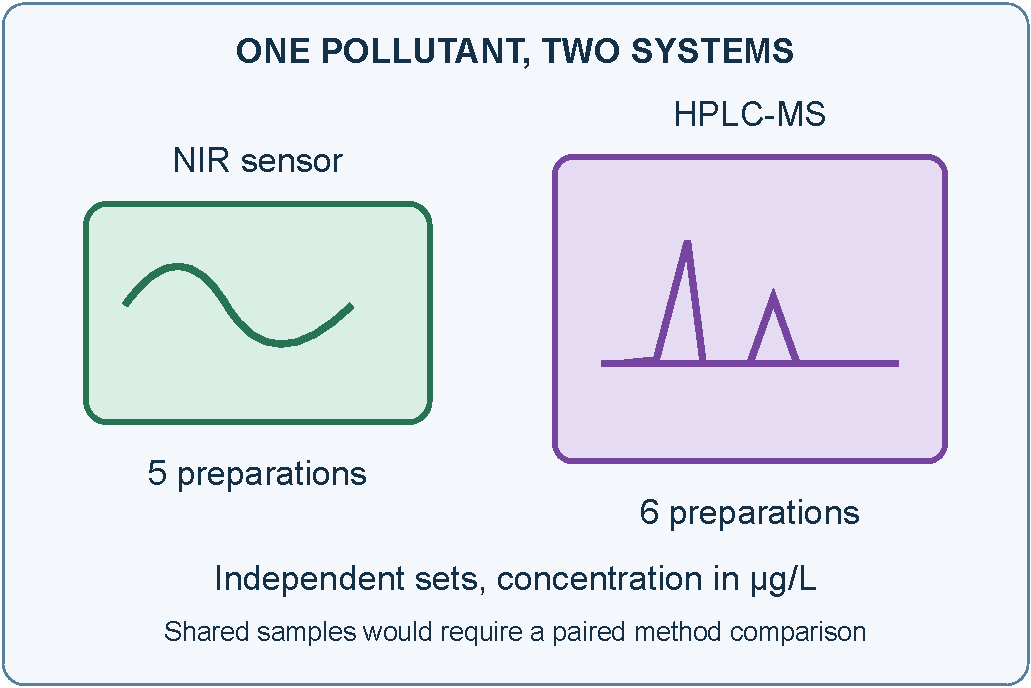
\includegraphics[width=\linewidth,height=.62\textheight,keepaspectratio]{asset-99dbfd4005a9410e7f3688fa09bace2b836430caa7e46c9c61a9422c1ab4e782.pdf}\end{center}

\medskip

\par\medskip
\Needspace{10cm}
\refstepcounter{figure}\label{material-b4ea53f64452a50d49c4741496838ca77459fe1afebbc902f30b28e0942186de}
\noindent\textbf{Fig.~\ref*{material-b4ea53f64452a50d49c4741496838ca77459fe1afebbc902f30b28e0942186de}.} Every independent concentration observation remains in its system group.\par\nopagebreak
\begin{center}
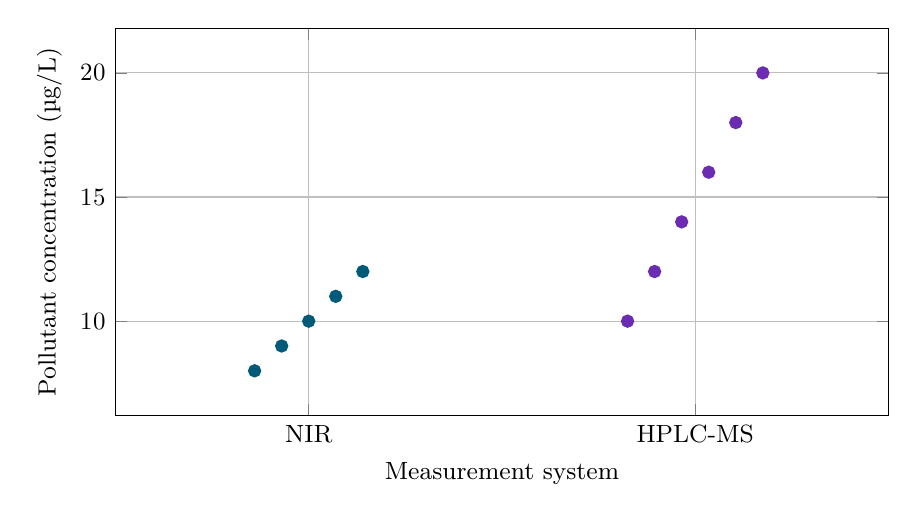
\begin{tikzpicture}
\begin{axis}[width=0.94\linewidth,
height=6.5cm,
scale only axis=false,
grid=major,
tick label style={font=\small},
label style={font=\small},
xlabel={Measurement system},
ylabel={Pollutant concentration (µg/L)},
legend style={font=\footnotesize,draw=none,at={(0.5,-0.28)},anchor=north,legend columns=1,text width=0.85\linewidth,align=left},
unbounded coords=jump,
scaled ticks=false,
ymin=6.2,
ymax=21.8,
xmin=0.5,
xmax=2.5,
xtick={1,2},
xticklabels={{NIR},{HPLC-MS}}]
\addplot[color=pcd1,thick,only marks,mark=*] coordinates {(0.86,8) (0.9299999999999999,9) (1,10) (1.07,11) (1.1400000000000001,12)};
\addplot[color=pcd2,thick,only marks,mark=*] coordinates {(1.825,10) (1.895,12) (1.965,14) (2.035,16) (2.105,18) (2.175,20)};

\end{axis}
\end{tikzpicture}
\end{center}


\medskip

\par\medskip
\Needspace{8\baselineskip}
\refstepcounter{scripttable}\label{material-208e0fd84411d4dcfede0de78aa9bfa57e6d79e60db66e2647ab1eed0a22c302}
\noindent\textbf{Table~\ref*{material-208e0fd84411d4dcfede0de78aa9bfa57e6d79e60db66e2647ab1eed0a22c302}.} Welch R-style report, approximate \ensuremath{\nu}, two-sided p and mean difference.\par\nopagebreak
\begin{longtable}{@{}p{\dimexpr0.500000\linewidth-2\tabcolsep\relax}p{\dimexpr0.500000\linewidth-2\tabcolsep\relax}@{}}
Field & Result \\ \hline
\endhead
Hypotheses & H\ensuremath{{}_0}: equal population means; H\ensuremath{{}_1}: different \\ \hline
Statistic / \ensuremath{\nu} / p & t = \ensuremath{-}2.9704; \ensuremath{\nu} \ensuremath{\approx} 6.972; two-sided p \ensuremath{\approx} 0.02089 \\ \hline
Mean estimates & NIR 10 µg/L (n 5); HPLC-MS 15 µg/L (n 6) \\ \hline
Mean difference & NIR minus HPLC-MS: \ensuremath{-}5 µg/L \\ \hline
Decision / model & Reject equal population means at 5\%; independent Normal groups, unequal variances permitted. Accuracy needs separate reference evidence. \\ \hline
\end{longtable}
\medskip

\par\medskip
\Needspace{10cm}
\refstepcounter{figure}\label{material-c75d95ca59c1d780eb96008b60ae04bc4671cf6f23aa115926e8043b71c83071}
\noindent\textbf{Fig.~\ref*{material-c75d95ca59c1d780eb96008b60ae04bc4671cf6f23aa115926e8043b71c83071}.} NIST: independent and paired t comparisons.\par\nopagebreak
\noindent\href{https://www.itl.nist.gov/div898/handbook/eda/section3/eda353.htm}{NIST: paired, pooled and Welch t-tests}\par
\nolinkurl{https://www.itl.nist.gov/div898/handbook/eda/section3/eda353.htm}\par

\medskip

\clearpage
\section{Prespecification and a three-claim test-family}
Good scientific practice starts with a population hypothesis, then plans the experiment and analysis before outcomes are known. Check assumptions, apply the prespecified procedure and report the result. Searching endpoints, directions, cutoffs or exclusions until p is small changes the error behaviour. Exploratory analyses can be useful when labelled honestly; they are not replacements for a confirmatory plan.


Consider independent replicate preparations from one water sample and three separate below-limit claims: chloride, bromate and phosphate, each against its own illustrative limit. Each H\ensuremath{{}_0} is at or above the limit and H\ensuremath{{}_1} below. The test-family error criterion here is at least one false below-limit claim. If all three nulls are true and the tests are independent, the chance of no false rejection is 0.95 cubed, or 0.857375. Thus at least one false rejection occurs with probability 0.142625, about 14.26\%. Shared sample preparation can make the tests dependent, so that exact rate is an example, not a universal answer. This is not the same decision problem as one joint claim that all analytes pass; a conjunctive pass-only rule has different error logic.


Bonferroni in \hyperref[material-f02c518c6a84f7fdcd3cf6f2ed40c41d2eaf2575dbfaf81afc30c7bbf96d83d7]{Eq.~\ref*{material-f02c518c6a84f7fdcd3cf6f2ed40c41d2eaf2575dbfaf81afc30c7bbf96d83d7}} divides the chosen 5\% test-family level by three, or equivalently multiplies valid raw p-values by three and caps at one. Use only one route. Its union bound permits dependence. The illustrative table \hyperref[material-761a1009dac04e4e53ca98607528e8074cfdd882bacb365d752fcc6dc97e62a9]{Table~\ref*{material-761a1009dac04e4e53ca98607528e8074cfdd882bacb365d752fcc6dc97e62a9}} has raw values \textbf{0.008, 0.021, 0.200}, adjusted to \textbf{0.024, 0.063, 0.600}. Only chloride supports a below-limit claim on this rule. Holm is another prespecified family-wise procedure: sort p, use successive thresholds 0.05/3, 0.05/2 and 0.05, and stop at the first failure. Here its adjusted values are 0.024, 0.042 and 0.200. Choose the procedure in advance. The experiment schematic \hyperref[material-142cce8825073fd475c805ca99d8ecec0c4a8b018675989f63641e64700c6c10]{Fig.~\ref*{material-142cce8825073fd475c805ca99d8ecec0c4a8b018675989f63641e64700c6c10}} makes the three replicate series explicit.


\par\medskip
\noindent\begin{minipage}{\linewidth}
\refstepcounter{equation}\label{material-f02c518c6a84f7fdcd3cf6f2ed40c41d2eaf2575dbfaf81afc30c7bbf96d83d7}
\noindent\textbf{Eq.~\ref*{material-f02c518c6a84f7fdcd3cf6f2ed40c41d2eaf2575dbfaf81afc30c7bbf96d83d7}.} Bonferroni controls at least one false rejection in a prespecified test-family.\par\nopagebreak
\begin{center}\begin{adjustbox}{max width=\linewidth}$\displaystyle \alpha_j=\frac{\alpha_{\mathrm{family}}}{m},\qquad p_{j,\mathrm{adj}}=\min(1,mp_j)$\end{adjustbox}\end{center}

\par\noindent\textbf{Symbols}

\begin{itemize}\setlength{\itemsep}{1pt}\setlength{\parsep}{0pt}
\item \textbf{\ensuremath{\alpha}\_family}: Chosen test-family significance level, here 0.05.
\item \textbf{m}: Number of planned tests, here three; positive integer.
\item \textbf{j}: One test's index.
\item \textbf{\ensuremath{\alpha}\_j}: Per-test significance level.
\item \textbf{p\_j; p\_j,adj}: Valid raw p-value; adjusted p-value.
\item \textbf{min}: Choose the smaller of the two arguments.
\item \textbf{mp\_j}: Multiplication of m and the raw p-value.
\item \textbf{/, =, parentheses}: Divide, equal, group arguments.
\end{itemize}

All levels and probabilities are dimensionless. Test-family membership is prespecified. The union-bound control permits dependent tests; it controls at least one false rejection, not every possible joint decision rule.

\end{minipage}\par
\medskip

\par\medskip
\Needspace{8\baselineskip}
\refstepcounter{scripttable}\label{material-761a1009dac04e4e53ca98607528e8074cfdd882bacb365d752fcc6dc97e62a9}
\noindent\textbf{Table~\ref*{material-761a1009dac04e4e53ca98607528e8074cfdd882bacb365d752fcc6dc97e62a9}.} Three illustrative below-limit claims and their adjusted p-values.\par\nopagebreak
\begin{longtable}{@{}p{\dimexpr0.333333\linewidth-2\tabcolsep\relax}p{\dimexpr0.333333\linewidth-2\tabcolsep\relax}p{\dimexpr0.333333\linewidth-2\tabcolsep\relax}@{}}
Endpoint & Raw p & Bonferroni adjusted p \\ \hline
\endhead
Chloride below its limit & 0.008 & 0.024: reject at family 0.05 \\ \hline
Bromate below its limit & 0.021 & 0.063: do not reject \\ \hline
Phosphate below its limit & 0.200 & 0.600: do not reject \\ \hline
\end{longtable}
\medskip

\par\medskip
\Needspace{10cm}
\refstepcounter{figure}\label{material-142cce8825073fd475c805ca99d8ecec0c4a8b018675989f63641e64700c6c10}
\noindent\textbf{Fig.~\ref*{material-142cce8825073fd475c805ca99d8ecec0c4a8b018675989f63641e64700c6c10}.} One water sample, six preparations and three analytes.\par\nopagebreak
\begin{center}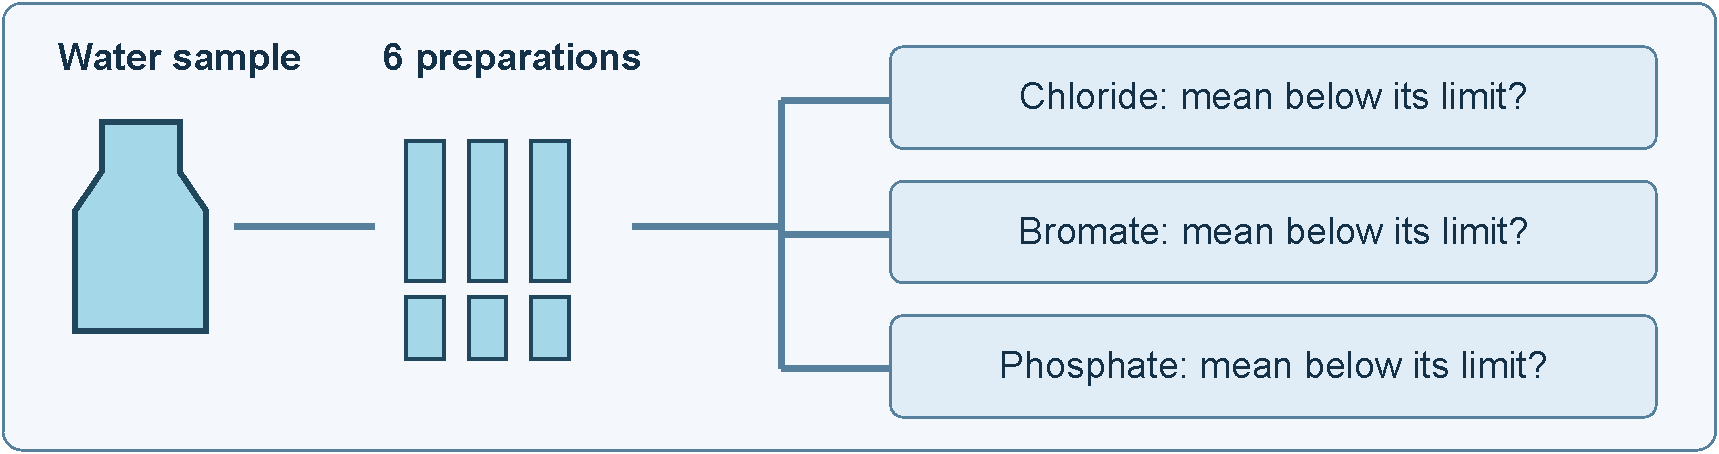
\includegraphics[width=\linewidth,height=.62\textheight,keepaspectratio]{asset-02206675af948a48680cd23e445818fae01f4f6c3258397326f644822edae753.pdf}\end{center}

\medskip

\clearpage
\section{F references for variances and nested calibration fits}
The F section marker \hyperref[material-939f1e657c65071c24f54be4bf8099700cc1d0fbc667927c77edb90549dfe6fa]{Fig.~\ref*{material-939f1e657c65071c24f54be4bf8099700cc1d0fbc667927c77edb90549dfe6fa}} opens comparisons of variances. As developed in Level 5, a ratio of independent Normal-sample variances has an F reference when population variances are equal. The \textbf{test statistic} \hyperref[material-d5198c5a5b27fac18ac8f0b0623a6c83859862fb336d3c7778b3f762c5f60a9b]{Eq.~\ref*{material-d5198c5a5b27fac18ac8f0b0623a6c83859862fb336d3c7778b3f762c5f60a9b}} keeps \textbf{\ensuremath{\nu}\ensuremath{{}_1} and \ensuremath{\nu}\ensuremath{{}_2}} in order. In the precision study \hyperref[material-1f66d2508a01c50eff4b83b2a444e48ec00b02d69872b21f0b222fcc399a8070]{Fig.~\ref*{material-1f66d2508a01c50eff4b83b2a444e48ec00b02d69872b21f0b222fcc399a8070}}, SDs \textbf{0.20 and 0.10 mg/L} yield a variance ratio \textbf{four}. Six independent preparations per method give \textbf{(\ensuremath{\nu}\ensuremath{{}_1}, \ensuremath{\nu}\ensuremath{{}_2}) = (5, 5)}. The NIST chapter \hyperref[material-4934b48f73e1757d565212bb617af0a4ae42afd91d5fa57c6ed9cc839f2f25ca]{Fig.~\ref*{material-4934b48f73e1757d565212bb617af0a4ae42afd91d5fa57c6ed9cc839f2f25ca}} explains this reference. The report \hyperref[material-d8adc661c1560270b0df20fa53558ee09e61acc18192f2710081d40cc0fe6338]{Table~\ref*{material-d8adc661c1560270b0df20fa53558ee09e61acc18192f2710081d40cc0fe6338}} gives \textbf{upper-tail p = 0.07719}: do not reject the equality boundary against greater A variance. Non-rejection cannot prove equal precision. Normality is especially important for this exact reference.


\par\medskip
\Needspace{10cm}
\refstepcounter{figure}\label{material-939f1e657c65071c24f54be4bf8099700cc1d0fbc667927c77edb90549dfe6fa}
\noindent\textbf{Fig.~\ref*{material-939f1e657c65071c24f54be4bf8099700cc1d0fbc667927c77edb90549dfe6fa}.} Variance-ratio theme of the F-test section.\par\nopagebreak
\begin{center}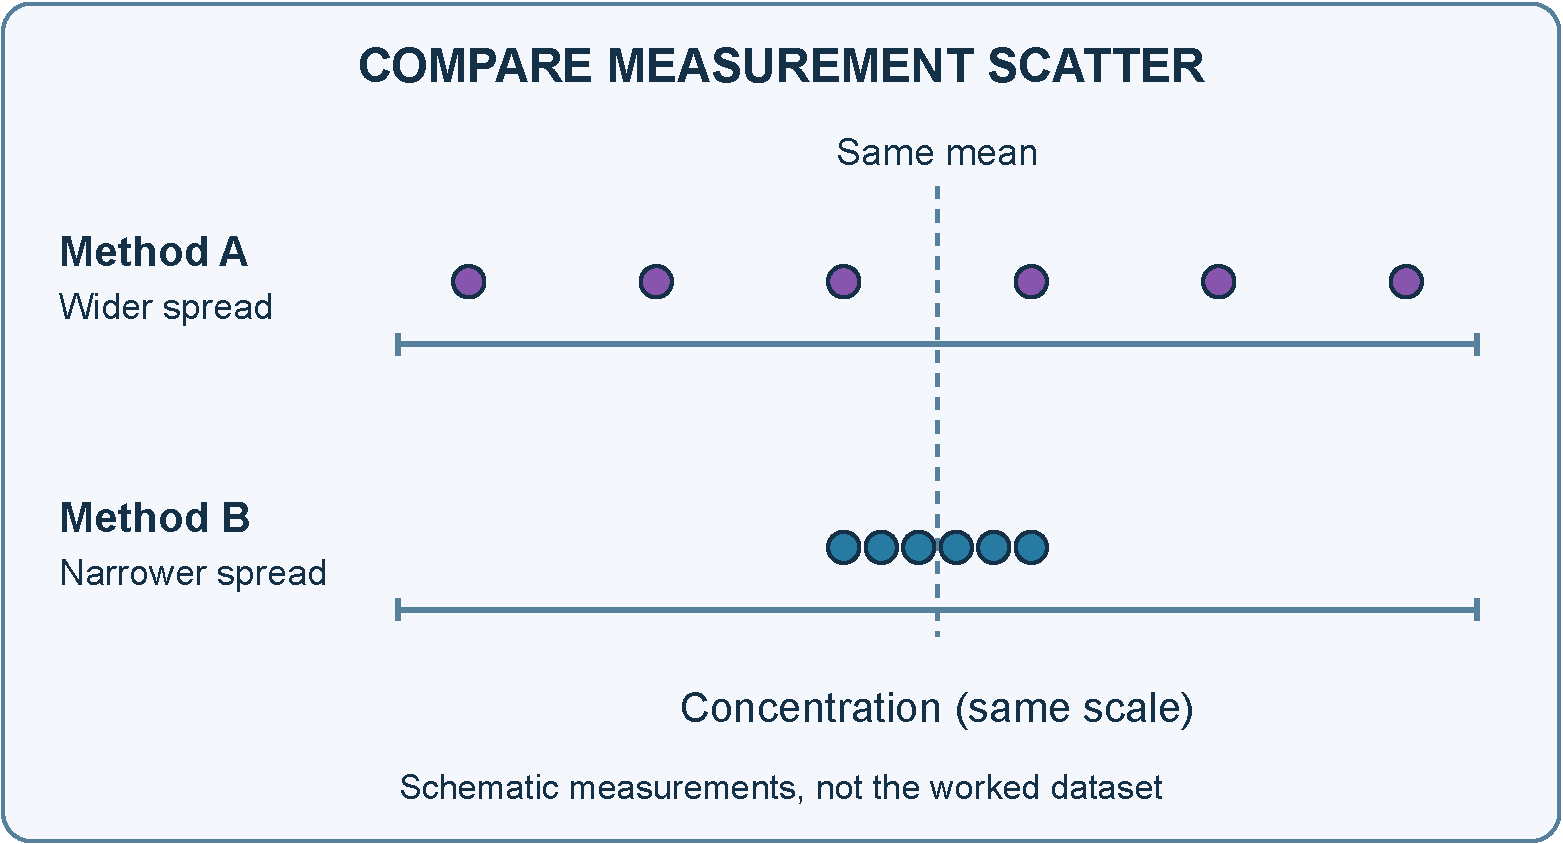
\includegraphics[width=\linewidth,height=.62\textheight,keepaspectratio]{asset-62df47582f4c3b377d2032221f2f32cea68496ed38e7eb15e8a83ac389e5a7a6.pdf}\end{center}

\medskip

\par\medskip
\noindent\begin{minipage}{\linewidth}
\refstepcounter{equation}\label{material-d5198c5a5b27fac18ac8f0b0623a6c83859862fb336d3c7778b3f762c5f60a9b}
\noindent\textbf{Eq.~\ref*{material-d5198c5a5b27fac18ac8f0b0623a6c83859862fb336d3c7778b3f762c5f60a9b}.} Prespecified variance-ratio orientation and ordered \ensuremath{\nu}\ensuremath{{}_1}, \ensuremath{\nu}\ensuremath{{}_2}.\par\nopagebreak
\begin{center}\begin{adjustbox}{max width=\linewidth}$\displaystyle F=\frac{s_1^2}{s_2^2},\qquad (\nu_1,\nu_2)=(n_1-1,n_2-1)$\end{adjustbox}\end{center}

\par\noindent\textbf{Symbols}

\begin{itemize}\setlength{\itemsep}{1pt}\setlength{\parsep}{0pt}
\item \textbf{F}: Observed variance ratio; dimensionless.
\item \textbf{s\ensuremath{{}_1}\ensuremath{{}^2}, s\ensuremath{{}_2}\ensuremath{{}^2}}: Sample variances, denominators n\ensuremath{{}_1} \ensuremath{-} 1 and n\ensuremath{{}_2} \ensuremath{-} 1; (mg/L)\ensuremath{{}^2}.
\item \textbf{1, 2}: Prespecified numerator A and denominator B.
\item \textbf{n\ensuremath{{}_1}, n\ensuremath{{}_2}}: Independent sample sizes, each greater than one.
\item \textbf{\ensuremath{\nu}\ensuremath{{}_1}, \ensuremath{\nu}\ensuremath{{}_2}}: Numerator and denominator degrees of freedom, in that order.
\item \textbf{2; \ensuremath{-}; =; fraction bar}: Square SD, subtract, equal, divide.
\item \textbf{Parentheses, comma}: Ordered pair of degrees of freedom.
\end{itemize}

Exact reference: independent Normal samples and equal positive population variances under H\ensuremath{{}_0}. The shown alternative is greater A variance, upper tail. A two-sided question needs both tails. Prespecify the ratio orientation.

\end{minipage}\par
\medskip

\par\medskip
\Needspace{10cm}
\refstepcounter{figure}\label{material-1f66d2508a01c50eff4b83b2a444e48ec00b02d69872b21f0b222fcc399a8070}
\noindent\textbf{Fig.~\ref*{material-1f66d2508a01c50eff4b83b2a444e48ec00b02d69872b21f0b222fcc399a8070}.} Six independent preparations per method and SD versus variance ratios.\par\nopagebreak
\begin{center}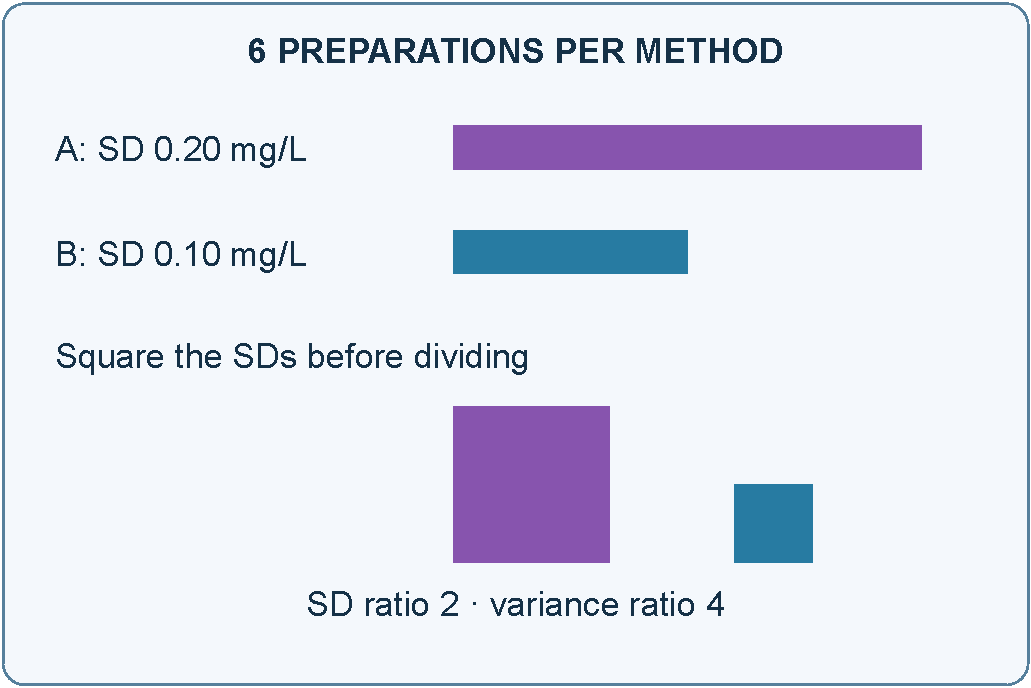
\includegraphics[width=\linewidth,height=.62\textheight,keepaspectratio]{asset-aec6db4e50869c75dd3bfc8c10c2c4a7538c66b83ea760ff7e1f033f43061190.pdf}\end{center}

\medskip

\par\medskip
\Needspace{10cm}
\refstepcounter{figure}\label{material-4934b48f73e1757d565212bb617af0a4ae42afd91d5fa57c6ed9cc839f2f25ca}
\noindent\textbf{Fig.~\ref*{material-4934b48f73e1757d565212bb617af0a4ae42afd91d5fa57c6ed9cc839f2f25ca}.} NIST reference for comparing variances with F.\par\nopagebreak
\noindent\href{https://www.itl.nist.gov/div898/handbook/eda/section3/eda359.htm}{NIST: comparison of variances}\par
\nolinkurl{https://www.itl.nist.gov/div898/handbook/eda/section3/eda359.htm}\par

\medskip

\par\medskip
\Needspace{8\baselineskip}
\refstepcounter{scripttable}\label{material-d8adc661c1560270b0df20fa53558ee09e61acc18192f2710081d40cc0fe6338}
\noindent\textbf{Table~\ref*{material-d8adc661c1560270b0df20fa53558ee09e61acc18192f2710081d40cc0fe6338}.} Upper-tail variance-comparison report, p 0.07719.\par\nopagebreak
\begin{longtable}{@{}p{\dimexpr0.500000\linewidth-2\tabcolsep\relax}p{\dimexpr0.500000\linewidth-2\tabcolsep\relax}@{}}
Field & Result \\ \hline
\endhead
Hypotheses & H\ensuremath{{}_0}: equal population variances; H\ensuremath{{}_1}: A greater than B \\ \hline
F / (\ensuremath{\nu}\ensuremath{{}_1}, \ensuremath{\nu}\ensuremath{{}_2}) / p & F = 4; (\ensuremath{\nu}\ensuremath{{}_1}, \ensuremath{\nu}\ensuremath{{}_2}) = (5, 5); upper-tail p = 0.07719 \\ \hline
Estimates & Variance A 0.040, B 0.010 (mg/L)\ensuremath{{}^2}; ratio 4 \\ \hline
Decision / model & Do not reject at 5\%. Independent Normal samples; no proof of equal precision. \\ \hline
\end{longtable}
\medskip

An F-test can instead compare nested models fitted to the same observations. The schematic calibration \hyperref[material-9591cc21e7f79da96b6825ab7696a29f87e1dbc9ea3f06d30b6046ba177898a4]{Fig.~\ref*{material-9591cc21e7f79da96b6825ab7696a29f87e1dbc9ea3f06d30b6046ba177898a4}} contrasts a constant response with adding a concentration slope. Under the shared independent Normal-error model, one added coefficient gives F equal to the square of its corresponding coefficient t statistic. This F question detects either slope direction. It does not require two separate datasets or two unrelated raw variance estimates.


\par\medskip
\Needspace{10cm}
\refstepcounter{figure}\label{material-9591cc21e7f79da96b6825ab7696a29f87e1dbc9ea3f06d30b6046ba177898a4}
\noindent\textbf{Fig.~\ref*{material-9591cc21e7f79da96b6825ab7696a29f87e1dbc9ea3f06d30b6046ba177898a4}.} Flat model versus nonzero slope using the same standards; schematic geometry.\par\nopagebreak
\begin{center}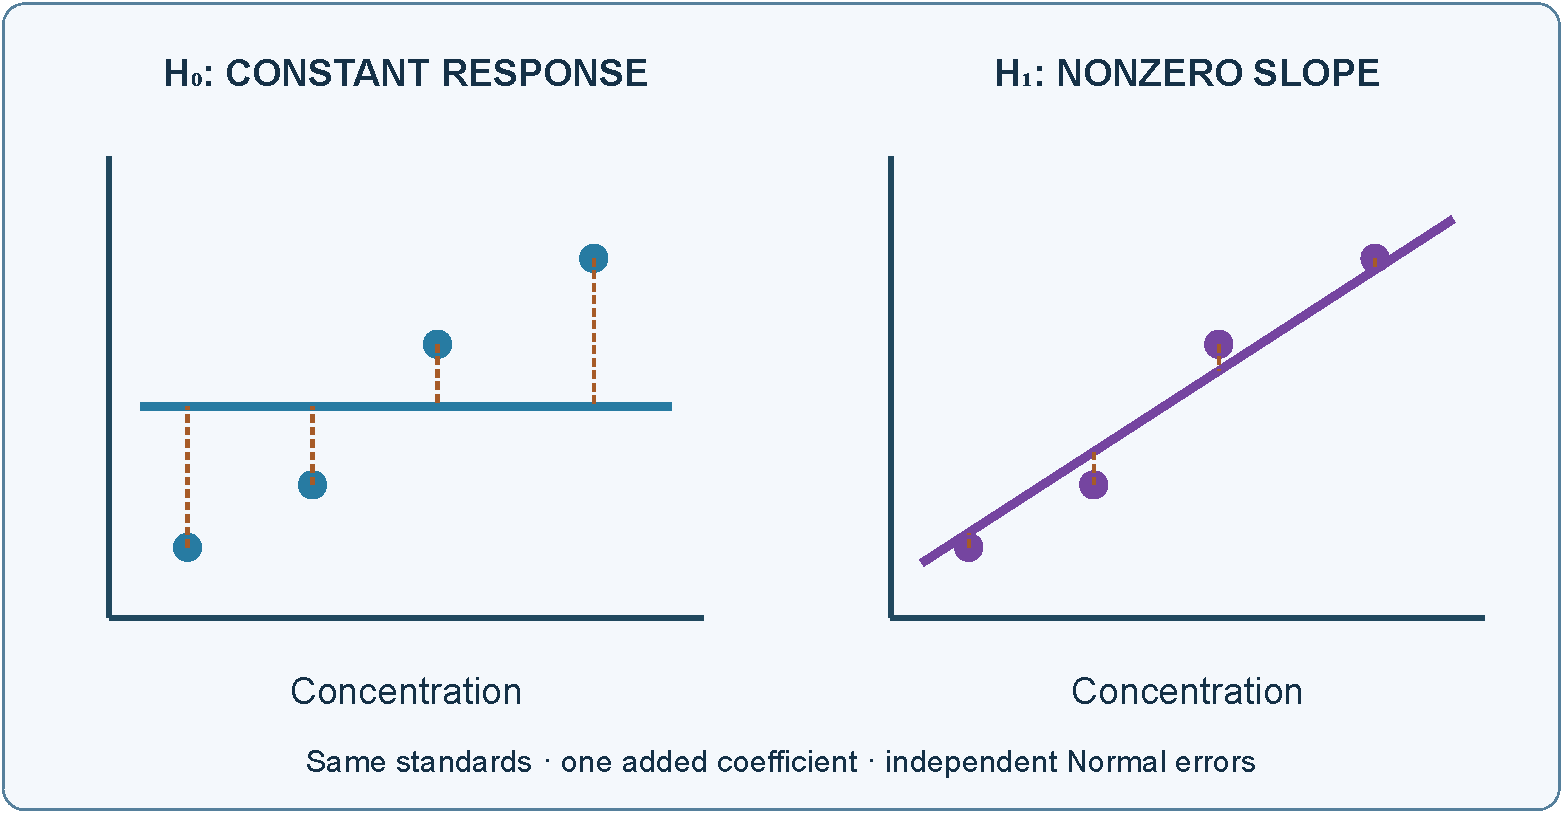
\includegraphics[width=\linewidth,height=.62\textheight,keepaspectratio]{asset-3b757aa9365e58342e7648866a86bc8f2b4eb507b152469930a4b85fb8ba887c.pdf}\end{center}

\medskip

Adding curvature to a straight line is another nested question. The formula \hyperref[material-1f87b72914014c8d7b2748782fa5a3f48daabbaf32d7160da2350dc2c48c82d2]{Eq.~\ref*{material-1f87b72914014c8d7b2748782fa5a3f48daabbaf32d7160da2350dc2c48c82d2}} compares error reduction per added coefficient with remaining full-model error per residual degree of freedom. The authored summary in \hyperref[material-988997b822b3275b2559d71de5a88cb5815751dd1ede8375bd0d53428eb73e0e]{Fig.~\ref*{material-988997b822b3275b2559d71de5a88cb5815751dd1ede8375bd0d53428eb73e0e}} uses ten standards, two versus three fitted coefficients, and RSS \textbf{12 versus 5}; the curves are conceptual. The report \hyperref[material-08bbcef0928a2a841f27eaaf39f3a75cd2f388285de5d29f60fb340d32286c4b]{Table~\ref*{material-08bbcef0928a2a841f27eaaf39f3a75cd2f388285de5d29f60fb340d32286c4b}} gives \textbf{F = 9.8, (\ensuremath{\nu}\ensuremath{{}_1}, \ensuremath{\nu}\ensuremath{{}_2}) = (1, 7), p = 0.01660}. Reject the zero-curvature coefficient under the shared Normal-error model. Residual checks and validation of the working range remain necessary. NIST describes related conditional coefficient tests in \hyperref[material-9d7f38e5ec5967241ec8f1588f250fe0162274049a622f3bfdd17eba82eddc00]{Fig.~\ref*{material-9d7f38e5ec5967241ec8f1588f250fe0162274049a622f3bfdd17eba82eddc00}}; for one added coefficient, the nested F equals its squared t statistic.


\par\medskip
\noindent\begin{minipage}{\linewidth}
\refstepcounter{equation}\label{material-1f87b72914014c8d7b2748782fa5a3f48daabbaf32d7160da2350dc2c48c82d2}
\noindent\textbf{Eq.~\ref*{material-1f87b72914014c8d7b2748782fa5a3f48daabbaf32d7160da2350dc2c48c82d2}.} Nested-model statistic from additional explained sum of squares and remaining error.\par\nopagebreak
\begin{center}\begin{adjustbox}{max width=\linewidth}$\displaystyle \begin{gathered}F=\frac{(\mathrm{RSS}_R-\mathrm{RSS}_F)/(p_F-p_R)}{\mathrm{RSS}_F/(n-p_F)}\\(\nu_1,\nu_2)=(p_F-p_R,n-p_F)\end{gathered}$\end{adjustbox}\end{center}

\par\noindent\textbf{Symbols}

\begin{itemize}\setlength{\itemsep}{1pt}\setlength{\parsep}{0pt}
\item \textbf{F}: Observed dimensionless test statistic.
\item \textbf{R, F subscripts}: Reduced and full model.
\item \textbf{RSS\_R, RSS\_F}: Residual sums of squares; squared response unit.
\item \textbf{p\_R, p\_F}: Fitted independent coefficients, including intercept; full has more.
\item \textbf{n}: Same observations in both models; exceeds full coefficient count.
\item \textbf{\ensuremath{\nu}\ensuremath{{}_1}, \ensuremath{\nu}\ensuremath{{}_2}}: Numerator and denominator degrees of freedom.
\item \textbf{\ensuremath{-}, =, fraction bars}: Subtract, equal, divide.
\item \textbf{Parentheses, comma}: Grouping and ordered degrees of freedom.
\end{itemize}

Exact reference: full-rank nested linear models; independent Normal errors with common positive variance. H\ensuremath{{}_0} sets added coefficients to zero. More flexible fits can explain random scatter; the F comparison calibrates the improvement.

\end{minipage}\par
\medskip

\par\medskip
\Needspace{10cm}
\refstepcounter{figure}\label{material-988997b822b3275b2559d71de5a88cb5815751dd1ede8375bd0d53428eb73e0e}
\noindent\textbf{Fig.~\ref*{material-988997b822b3275b2559d71de5a88cb5815751dd1ede8375bd0d53428eb73e0e}.} Authored line/curve RSS summaries 12 and 5 for ten standards.\par\nopagebreak
\begin{center}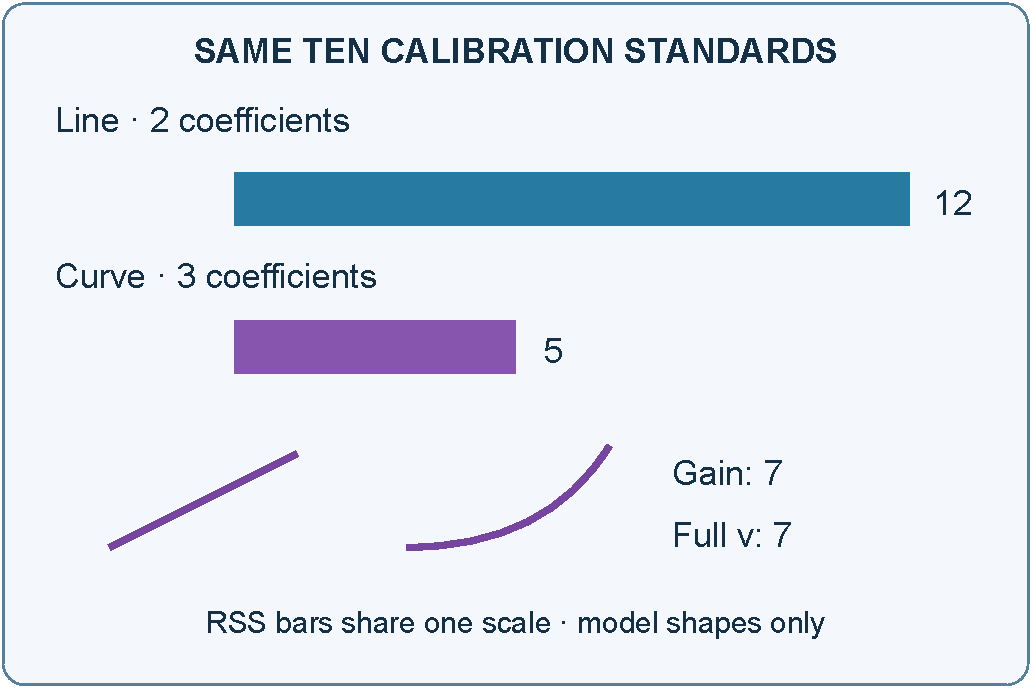
\includegraphics[width=\linewidth,height=.62\textheight,keepaspectratio]{asset-87dc866f51a72ed9ca57c8c00acf902f8fda29c0929b6d7895512974bc321e67.pdf}\end{center}

\medskip

\par\medskip
\Needspace{8\baselineskip}
\refstepcounter{scripttable}\label{material-08bbcef0928a2a841f27eaaf39f3a75cd2f388285de5d29f60fb340d32286c4b}
\noindent\textbf{Table~\ref*{material-08bbcef0928a2a841f27eaaf39f3a75cd2f388285de5d29f60fb340d32286c4b}.} Nested curvature-test report, with upper-tail p and model assumptions.\par\nopagebreak
\begin{longtable}{@{}p{\dimexpr0.500000\linewidth-2\tabcolsep\relax}p{\dimexpr0.500000\linewidth-2\tabcolsep\relax}@{}}
Field & Result \\ \hline
\endhead
Hypotheses & H\ensuremath{{}_0}: curve coefficient zero; H\ensuremath{{}_1}: nonzero \\ \hline
F / (\ensuremath{\nu}\ensuremath{{}_1}, \ensuremath{\nu}\ensuremath{{}_2}) / p & F = 9.8; (\ensuremath{\nu}\ensuremath{{}_1}, \ensuremath{\nu}\ensuremath{{}_2}) = (1, 7); upper-tail p = 0.01660 \\ \hline
Same ten standards & Line: 2 coefficients, RSS 12; curve: 3 coefficients, RSS 5 \\ \hline
Decision / model & Reject at 5\%; independent Normal errors, common variance, nested full-rank fits. Inspect residuals and working range too. \\ \hline
\end{longtable}
\medskip

\par\medskip
\Needspace{10cm}
\refstepcounter{figure}\label{material-9d7f38e5ec5967241ec8f1588f250fe0162274049a622f3bfdd17eba82eddc00}
\noindent\textbf{Fig.~\ref*{material-9d7f38e5ec5967241ec8f1588f250fe0162274049a622f3bfdd17eba82eddc00}.} NIST: conditional regression coefficient tests.\par\nopagebreak
\noindent\href{https://www.itl.nist.gov/div898/handbook/pmd/section4/pmd447.htm}{NIST: regression coefficient tests}\par
\nolinkurl{https://www.itl.nist.gov/div898/handbook/pmd/section4/pmd447.htm}\par

\medskip

\clearpage
\section{Three distinct chi-square questions}
The overview \hyperref[material-59e658203ee093c3a0acf4923d68d6bced64a648b419c865b210daf5689a9ae6]{Fig.~\ref*{material-59e658203ee093c3a0acf4923d68d6bced64a648b419c865b210daf5689a9ae6}} separates a numeric variance question from two questions about counts. For a fixed known target variance, the setup \hyperref[material-a7e82a3d7ddbdd058e2e6cc5d3bf6f5864834fbdb7cc1bd76b7c99c5bb1883dc]{Fig.~\ref*{material-a7e82a3d7ddbdd058e2e6cc5d3bf6f5864834fbdb7cc1bd76b7c99c5bb1883dc}} leads to \hyperref[material-c3f66b94b26ecb4e28d017577365389ce0450c6d7c23b1c2717b19f140ae8eca]{Eq.~\ref*{material-c3f66b94b26ecb4e28d017577365389ce0450c6d7c23b1c2717b19f140ae8eca}}, an exact Normal-model reference. The six results in \hyperref[material-cf03ea569f2f9952bd337dcb6d49ab3244f6e56251d8906283fae9ac15390612]{Fig.~\ref*{material-cf03ea569f2f9952bd337dcb6d49ab3244f6e56251d8906283fae9ac15390612}} have sample variance \textbf{0.024 (mg/L)\ensuremath{{}^2}}. A known SD target \textbf{0.10 mg/L} gives variance \textbf{0.010 (mg/L)\ensuremath{{}^2}}. Multiply by \textbf{\ensuremath{\nu} = 5} and divide by the target: \textbf{Q = 12}. The report \hyperref[material-76053d0f4f50f1222f13a6fa72ac60ffb3d6ecc0b95344c775ab130d57d6bdbc]{Table~\ref*{material-76053d0f4f50f1222f13a6fa72ac60ffb3d6ecc0b95344c775ab130d57d6bdbc}} gives \textbf{upper-tail p = 0.03479}, evidence of excess variance at 5\%. A separately estimated target requires an analysis including its uncertainty.


\par\medskip
\Needspace{10cm}
\refstepcounter{figure}\label{material-59e658203ee093c3a0acf4923d68d6bced64a648b419c865b210daf5689a9ae6}
\noindent\textbf{Fig.~\ref*{material-59e658203ee093c3a0acf4923d68d6bced64a648b419c865b210daf5689a9ae6}.} Measurement scatter, particle composition and classification association are different questions.\par\nopagebreak
\begin{center}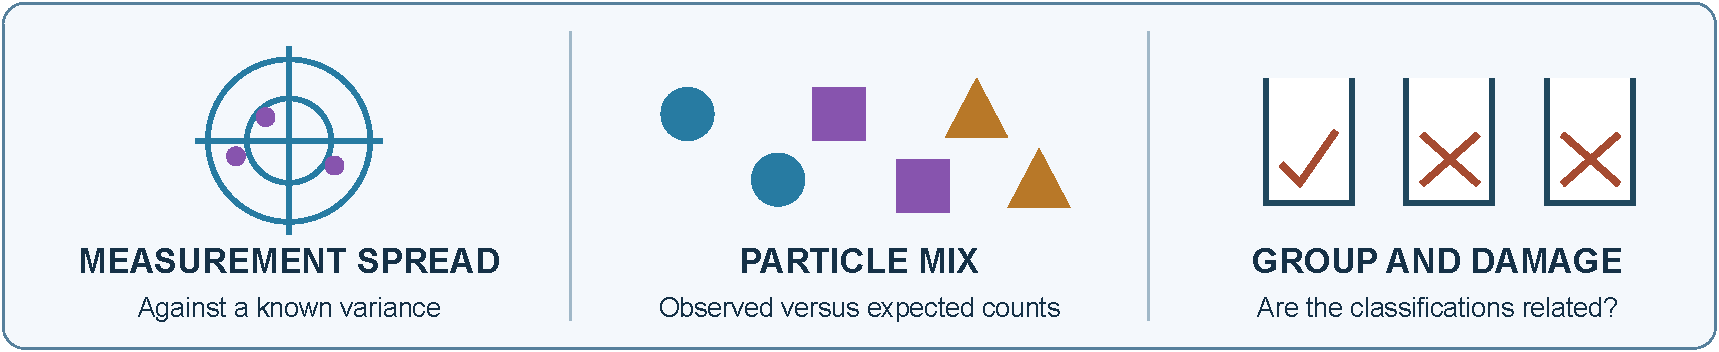
\includegraphics[width=\linewidth,height=.62\textheight,keepaspectratio]{asset-1730fee3aecb256a0a284f7362de02f17cc21ead93c5b03a7aeca41ab4548d3c.pdf}\end{center}

\medskip

\par\medskip
\Needspace{10cm}
\refstepcounter{figure}\label{material-a7e82a3d7ddbdd058e2e6cc5d3bf6f5864834fbdb7cc1bd76b7c99c5bb1883dc}
\noindent\textbf{Fig.~\ref*{material-a7e82a3d7ddbdd058e2e6cc5d3bf6f5864834fbdb7cc1bd76b7c99c5bb1883dc}.} One independently measured series against a known variance target.\par\nopagebreak
\begin{center}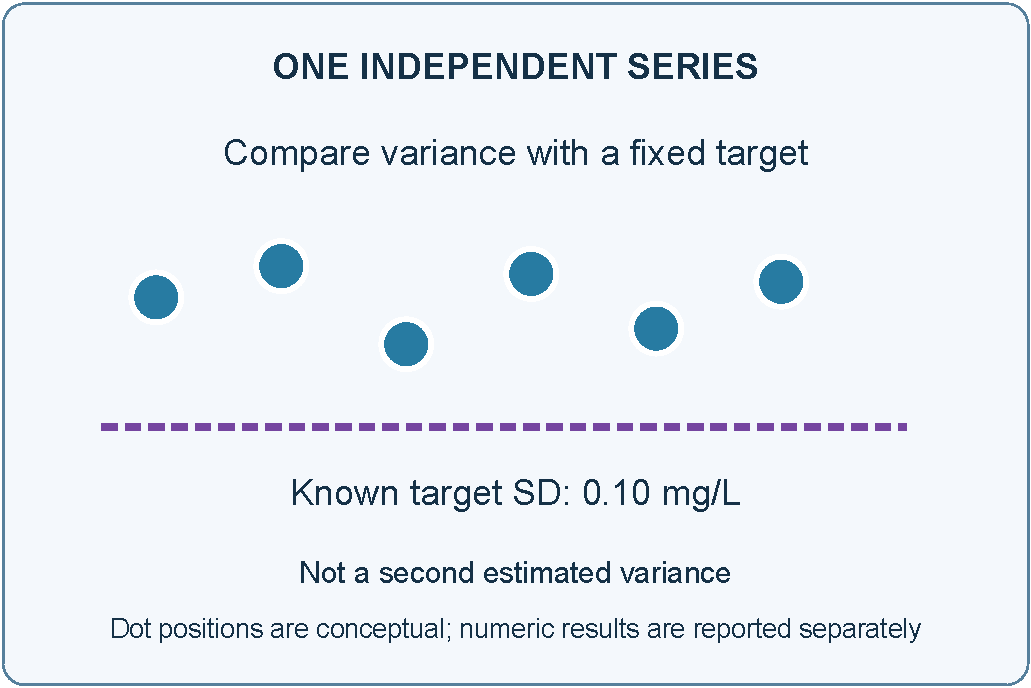
\includegraphics[width=\linewidth,height=.62\textheight,keepaspectratio]{asset-1663a4515991f318e224e9af7914caa1b81c0e8f2bc1bfd736763e9cc43898d8.pdf}\end{center}

\medskip

\par\medskip
\noindent\begin{minipage}{\linewidth}
\refstepcounter{equation}\label{material-c3f66b94b26ecb4e28d017577365389ce0450c6d7c23b1c2717b19f140ae8eca}
\noindent\textbf{Eq.~\ref*{material-c3f66b94b26ecb4e28d017577365389ce0450c6d7c23b1c2717b19f140ae8eca}.} Exact known-variance Normal-model statistic.\par\nopagebreak
\begin{center}\begin{adjustbox}{max width=\linewidth}$\displaystyle Q=\frac{(n-1)s^2}{\sigma_0^2},\qquad \nu=n-1$\end{adjustbox}\end{center}

\par\noindent\textbf{Symbols}

\begin{itemize}\setlength{\itemsep}{1pt}\setlength{\parsep}{0pt}
\item \textbf{Q}: Observed chi-square statistic; dimensionless.
\item \textbf{n}: Number of independent measurements, greater than one.
\item \textbf{\ensuremath{\nu}}: Residual degrees of freedom.
\item \textbf{s\ensuremath{{}^2}}: Sample variance, denominator n \ensuremath{-} 1; (mg/L)\ensuremath{{}^2}.
\item \textbf{\ensuremath{\sigma}\ensuremath{{}_0}\ensuremath{{}^2}}: Known positive target population variance; (mg/L)\ensuremath{{}^2}.
\item \textbf{0; 2}: Null-reference subscript; exponent squares SD.
\item \textbf{\ensuremath{-}, =, fraction bar}: Subtract, equal, divide.
\item \textbf{Juxtaposition; parentheses}: Multiply; group n \ensuremath{-} 1.
\end{itemize}

Exact reference assumes independent identically distributed Normal measurements and a fixed target variance. For an at-or-below null, use equality as the upper-tail boundary. An estimated reference variance instead needs a two-sample model.

\end{minipage}\par
\medskip

\par\medskip
\Needspace{10cm}
\refstepcounter{figure}\label{material-cf03ea569f2f9952bd337dcb6d49ab3244f6e56251d8906283fae9ac15390612}
\noindent\textbf{Fig.~\ref*{material-cf03ea569f2f9952bd337dcb6d49ab3244f6e56251d8906283fae9ac15390612}.} Six synthetic measurements with observed variance 0.024 (mg/L)\ensuremath{{}^2}.\par\nopagebreak
\begin{center}
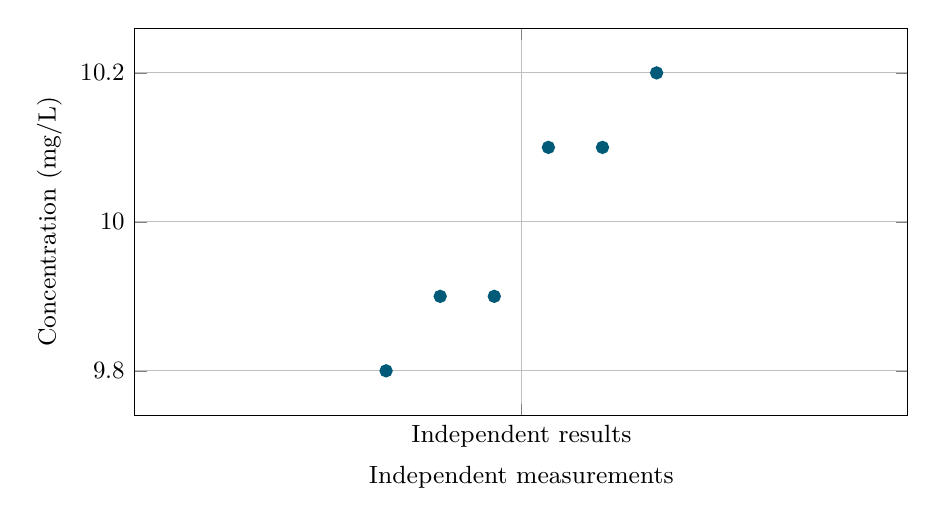
\begin{tikzpicture}
\begin{axis}[width=0.94\linewidth,
height=6.5cm,
scale only axis=false,
grid=major,
tick label style={font=\small},
label style={font=\small},
xlabel={Independent measurements},
ylabel={Concentration (mg/L)},
legend style={font=\footnotesize,draw=none,at={(0.5,-0.28)},anchor=north,legend columns=1,text width=0.85\linewidth,align=left},
unbounded coords=jump,
scaled ticks=false,
ymin=9.74,
ymax=10.26,
xmin=0.5,
xmax=1.5,
xtick={1},
xticklabels={{Independent results}}]
\addplot[color=pcd1,thick,only marks,mark=*] coordinates {(0.825,9.8) (0.895,9.9) (0.965,9.9) (1.035,10.1) (1.105,10.1) (1.175,10.2)};

\end{axis}
\end{tikzpicture}
\end{center}


\medskip

\par\medskip
\Needspace{8\baselineskip}
\refstepcounter{scripttable}\label{material-76053d0f4f50f1222f13a6fa72ac60ffb3d6ecc0b95344c775ab130d57d6bdbc}
\noindent\textbf{Table~\ref*{material-76053d0f4f50f1222f13a6fa72ac60ffb3d6ecc0b95344c775ab130d57d6bdbc}.} One-variance report with upper-tail p.\par\nopagebreak
\begin{longtable}{@{}p{\dimexpr0.500000\linewidth-2\tabcolsep\relax}p{\dimexpr0.500000\linewidth-2\tabcolsep\relax}@{}}
Field & Result \\ \hline
\endhead
Hypotheses & H\ensuremath{{}_0}: variance at or below 0.010 (mg/L)\ensuremath{{}^2}; H\ensuremath{{}_1}: above \\ \hline
Statistic / \ensuremath{\nu} / p & Q = 12; \ensuremath{\nu} = 5; upper-tail p = 0.03479 \\ \hline
Sample / reference & n = 6; variance 0.024 (mg/L)\ensuremath{{}^2}; known target SD 0.10 mg/L \\ \hline
Decision / model & Reject at 5\%; independent Normal observations, known fixed target. Evidence of excess scatter. \\ \hline
\end{longtable}
\medskip

For particle categories, Pearson's \textbf{test statistic} \hyperref[material-7cff151be3243992b6c6f60a2ac55ac47c8e18f710a38ae76d67017f5ef6c595]{Eq.~\ref*{material-7cff151be3243992b6c6f60a2ac55ac47c8e18f710a38ae76d67017f5ef6c595}} adds squared observed-minus-expected count differences divided by expected count. The bars \hyperref[material-d19fe486005c011284611a3da7aed76bb75e54f055acd965ae3817d645d1a644]{Fig.~\ref*{material-d19fe486005c011284611a3da7aed76bb75e54f055acd965ae3817d645d1a644}} retain \textbf{60 independent particles}: observed \textbf{30,20,10}, expected \textbf{30,18,12} from fixed shares \textbf{50\%,30\%,20\%}. The report \hyperref[material-9179bcecdb886c835cb5eb5b7e8b599282e219c76e7066a30642062d0a7c9ab3]{Table~\ref*{material-9179bcecdb886c835cb5eb5b7e8b599282e219c76e7066a30642062d0a7c9ab3}} gives \textbf{X\ensuremath{{}^2} = 0.5556, \ensuremath{\nu} = 2, approximate upper-tail p = 0.7575}. Do not reject the mix; this cannot prove its shares. Categories must be exhaustive and mutually exclusive. Fitted shares or sparse expectations require suitable calibration.


\par\medskip
\noindent\begin{minipage}{\linewidth}
\refstepcounter{equation}\label{material-7cff151be3243992b6c6f60a2ac55ac47c8e18f710a38ae76d67017f5ef6c595}
\noindent\textbf{Eq.~\ref*{material-7cff151be3243992b6c6f60a2ac55ac47c8e18f710a38ae76d67017f5ef6c595}.} Pearson category-count discrepancy and fixed-probability \ensuremath{\nu}.\par\nopagebreak
\begin{center}\begin{adjustbox}{max width=\linewidth}$\displaystyle \begin{gathered}X^2=\sum_{j=1}^{k}\frac{(O_j-E_j)^2}{E_j}\\E_j=N\pi_j,\qquad \nu=k-1\end{gathered}$\end{adjustbox}\end{center}

\par\noindent\textbf{Symbols}

\begin{itemize}\setlength{\itemsep}{1pt}\setlength{\parsep}{0pt}
\item \textbf{X\ensuremath{{}^2}}: Dimensionless Pearson statistic.
\item \textbf{j; k}: Category index; number of exhaustive, mutually exclusive categories.
\item \textbf{O\_j; E\_j}: Observed count; positive null expected count.
\item \textbf{N}: Total independent particles.
\item \textbf{\ensuremath{\pi}\_j}: Fixed category probability; all probabilities add to one.
\item \textbf{\ensuremath{\nu}}: Approximate reference degrees of freedom with fixed probabilities.
\item \textbf{\ensuremath{\Sigma}}: Sum over categories 1 through k.
\item \textbf{2, \ensuremath{-}, =, fraction bars}: Square, subtract, equal, divide.
\end{itemize}

Counts, probabilities and statistic are dimensionless. Juxtaposition multiplies; parentheses group. Adequate expected counts support the chi-square approximation. Fitted probabilities require adjusted degrees of freedom and calibration.

\end{minipage}\par
\medskip

\par\medskip
\Needspace{10cm}
\refstepcounter{figure}\label{material-d19fe486005c011284611a3da7aed76bb75e54f055acd965ae3817d645d1a644}
\noindent\textbf{Fig.~\ref*{material-d19fe486005c011284611a3da7aed76bb75e54f055acd965ae3817d645d1a644}.} Observed versus predicted category counts on a shared scale.\par\nopagebreak
\begin{center}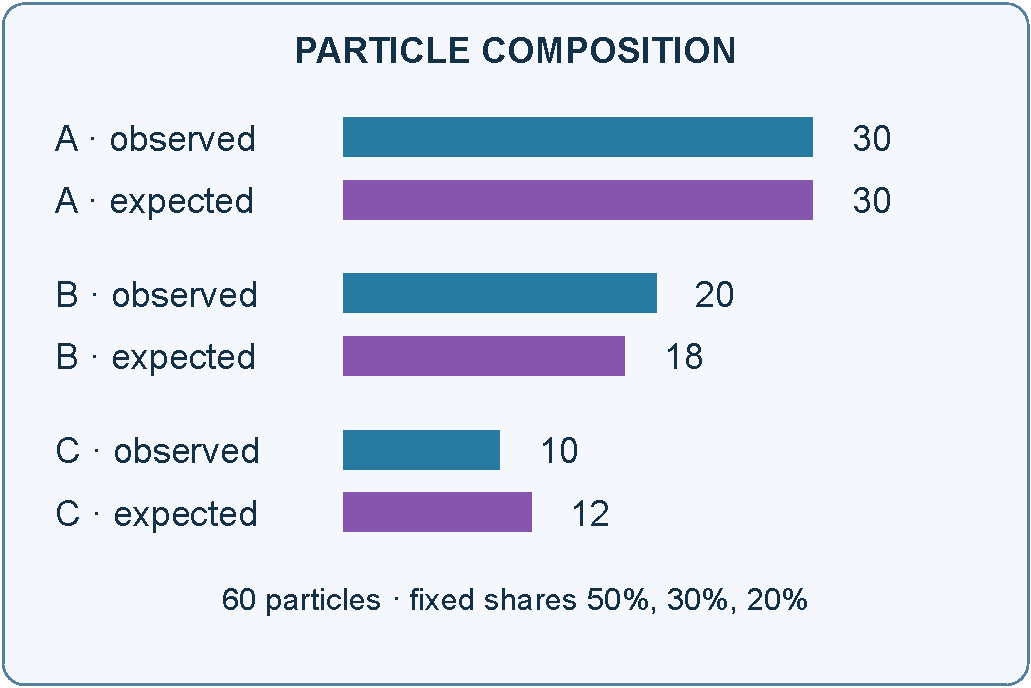
\includegraphics[width=\linewidth,height=.62\textheight,keepaspectratio]{asset-a1f7c9b339509a93bbb7258be9163b11526925b9de318d9259c9e572c92b720c.pdf}\end{center}

\medskip

\par\medskip
\Needspace{8\baselineskip}
\refstepcounter{scripttable}\label{material-9179bcecdb886c835cb5eb5b7e8b599282e219c76e7066a30642062d0a7c9ab3}
\noindent\textbf{Table~\ref*{material-9179bcecdb886c835cb5eb5b7e8b599282e219c76e7066a30642062d0a7c9ab3}.} Goodness-of-fit report with approximate chi-square reference.\par\nopagebreak
\begin{longtable}{@{}p{\dimexpr0.500000\linewidth-2\tabcolsep\relax}p{\dimexpr0.500000\linewidth-2\tabcolsep\relax}@{}}
Field & Result \\ \hline
\endhead
Hypotheses & H\ensuremath{{}_0}: proportions 50\%, 30\%, 20\%; H\ensuremath{{}_1}: a different mix \\ \hline
Statistic / \ensuremath{\nu} / p & Pearson X\ensuremath{{}^2} = 0.5556; \ensuremath{\nu} = 2; upper-tail approximate p = 0.7575 \\ \hline
Observed / expected & 30, 20, 10 / 30, 18, 12; 60 independent particles \\ \hline
Decision / model & Do not reject at 5\%. Fixed multinomial probabilities, adequate expected counts. No proof of the mix. \\ \hline
\end{longtable}
\medskip

For group/damage independence, \hyperref[material-9acb48b2d655b252619d5a0cf7627f69d0cc1efdcc06a6b7ad2dd39184492de1]{Eq.~\ref*{material-9acb48b2d655b252619d5a0cf7627f69d0cc1efdcc06a6b7ad2dd39184492de1}} obtains expected cells from row and column totals. The synthetic table \hyperref[material-0f5550c94693e076e293ab18cb2226c799b834ea9b7c8f5ff2651a3aa77fa2b0]{Fig.~\ref*{material-0f5550c94693e076e293ab18cb2226c799b834ea9b7c8f5ff2651a3aa77fa2b0}} has control \textbf{8 affected/12 unaffected} and exposure \textbf{14/6}. Independence predicts \textbf{11 affected and 9 unaffected} in each group of twenty. The report \hyperref[material-9fae88414b0c633e7b74149802df50a5b3680a5f31720c468924223916c257d3]{Table~\ref*{material-9fae88414b0c633e7b74149802df50a5b3680a5f31720c468924223916c257d3}} uses uncorrected Pearson: \textbf{X\ensuremath{{}^2} = 3.6364, \ensuremath{\nu} = 1, approximate upper-tail p = 0.05653}. Do not reject at 5\%; this cannot prove independence. Every independent vessel enters one cell. The setup \hyperref[material-3cc18af9f3e657e434cff0bf5eea97227d1f0a2e9a225ab1e295a2d0e4a2379d]{Fig.~\ref*{material-3cc18af9f3e657e434cff0bf5eea97227d1f0a2e9a225ab1e295a2d0e4a2379d}} maps treatment to rows and classification to columns. R's default continuity correction gives a different statistic. Further reading: NIST variance \hyperref[material-fa79b678a3fcd687e0612266a93c9d5643681383321fc7ff5edb17686a8b8cf4]{Fig.~\ref*{material-fa79b678a3fcd687e0612266a93c9d5643681383321fc7ff5edb17686a8b8cf4}}, goodness of fit \hyperref[material-0020ebecabbc6660c149fbc34b9fff41ea856c0c43274464936460915f0429d0]{Fig.~\ref*{material-0020ebecabbc6660c149fbc34b9fff41ea856c0c43274464936460915f0429d0}}, and contingency tables \hyperref[material-1e5f142084e4de38141c9a5e144e022f873551e3b779bc3379fdd2cacac9d2ce]{Fig.~\ref*{material-1e5f142084e4de38141c9a5e144e022f873551e3b779bc3379fdd2cacac9d2ce}}.


\par\medskip
\noindent\begin{minipage}{\linewidth}
\refstepcounter{equation}\label{material-9acb48b2d655b252619d5a0cf7627f69d0cc1efdcc06a6b7ad2dd39184492de1}
\noindent\textbf{Eq.~\ref*{material-9acb48b2d655b252619d5a0cf7627f69d0cc1efdcc06a6b7ad2dd39184492de1}.} Independence-predicted cell counts and reference \ensuremath{\nu}.\par\nopagebreak
\begin{center}\begin{adjustbox}{max width=\linewidth}$\displaystyle \begin{gathered}X^2=\sum_{i=1}^{r}\sum_{j=1}^{c}\frac{(O_{ij}-E_{ij})^2}{E_{ij}}\\E_{ij}=\frac{R_i C_j}{N}\\\nu=(r-1)(c-1)\end{gathered}$\end{adjustbox}\end{center}

\par\noindent\textbf{Symbols}

\begin{itemize}\setlength{\itemsep}{1pt}\setlength{\parsep}{0pt}
\item \textbf{X\ensuremath{{}^2}}: Dimensionless Pearson discrepancy statistic.
\item \textbf{i, j; r, c}: Row/column indices; numbers of categories, each greater than one.
\item \textbf{O\_ij; E\_ij}: Observed cell count; positive expected count under independence.
\item \textbf{R\_i, C\_j}: Row total and column total.
\item \textbf{N}: Positive grand total of independent vessels.
\item \textbf{\ensuremath{\nu}}: Approximate reference degrees of freedom.
\item \textbf{Double \ensuremath{\Sigma}}: Sum over every row and column cell.
\item \textbf{2; juxtaposition; fraction bars}: Square, multiply, divide.
\item \textbf{\ensuremath{-}, =, parentheses}: Subtract, equal, group.
\end{itemize}

Counts, degrees of freedom and statistic are dimensionless. Each independent vessel enters one cell. Adequate expected counts support the chi-square approximation; sparse cells need suitable exact or simulation calibration. The vessel is the independent unit.

\end{minipage}\par
\medskip

\par\medskip
\Needspace{10cm}
\refstepcounter{figure}\label{material-0f5550c94693e076e293ab18cb2226c799b834ea9b7c8f5ff2651a3aa77fa2b0}
\noindent\textbf{Fig.~\ref*{material-0f5550c94693e076e293ab18cb2226c799b834ea9b7c8f5ff2651a3aa77fa2b0}.} Affected/unaffected vessel counts and their independence prediction.\par\nopagebreak
\begin{center}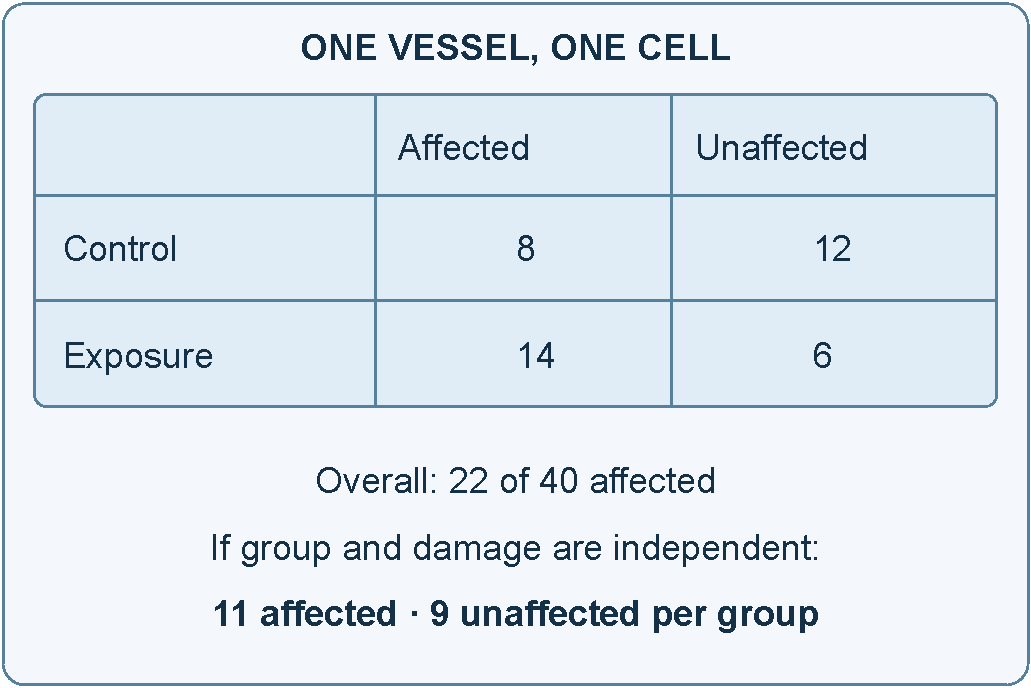
\includegraphics[width=\linewidth,height=.62\textheight,keepaspectratio]{asset-06b58931ee2ca28709d91df8c875e0c2aeb1a1572eb1a871d7f85e237138c3b6.pdf}\end{center}

\medskip

\par\medskip
\Needspace{8\baselineskip}
\refstepcounter{scripttable}\label{material-9fae88414b0c633e7b74149802df50a5b3680a5f31720c468924223916c257d3}
\noindent\textbf{Table~\ref*{material-9fae88414b0c633e7b74149802df50a5b3680a5f31720c468924223916c257d3}.} Uncorrected Pearson independence report, approximate p 0.05653.\par\nopagebreak
\begin{longtable}{@{}p{\dimexpr0.500000\linewidth-2\tabcolsep\relax}p{\dimexpr0.500000\linewidth-2\tabcolsep\relax}@{}}
Field & Result \\ \hline
\endhead
Hypotheses & H\ensuremath{{}_0}: group and damage independent; H\ensuremath{{}_1}: associated \\ \hline
Statistic / \ensuremath{\nu} / p & X\ensuremath{{}^2} = 3.6364; \ensuremath{\nu} = 1; upper-tail approximate p = 0.05653 \\ \hline
Convention / units & Uncorrected Pearson; 40 independent vessels; expected 11 affected / 9 unaffected per group \\ \hline
Decision at 5\% & Do not reject. Adequate expected counts support the approximation; not evidence of no association. \\ \hline
\end{longtable}
\medskip

\par\medskip
\Needspace{10cm}
\refstepcounter{figure}\label{material-3cc18af9f3e657e434cff0bf5eea97227d1f0a2e9a225ab1e295a2d0e4a2379d}
\noindent\textbf{Fig.~\ref*{material-3cc18af9f3e657e434cff0bf5eea97227d1f0a2e9a225ab1e295a2d0e4a2379d}.} How the vessels become table rows and columns.\par\nopagebreak
\begin{center}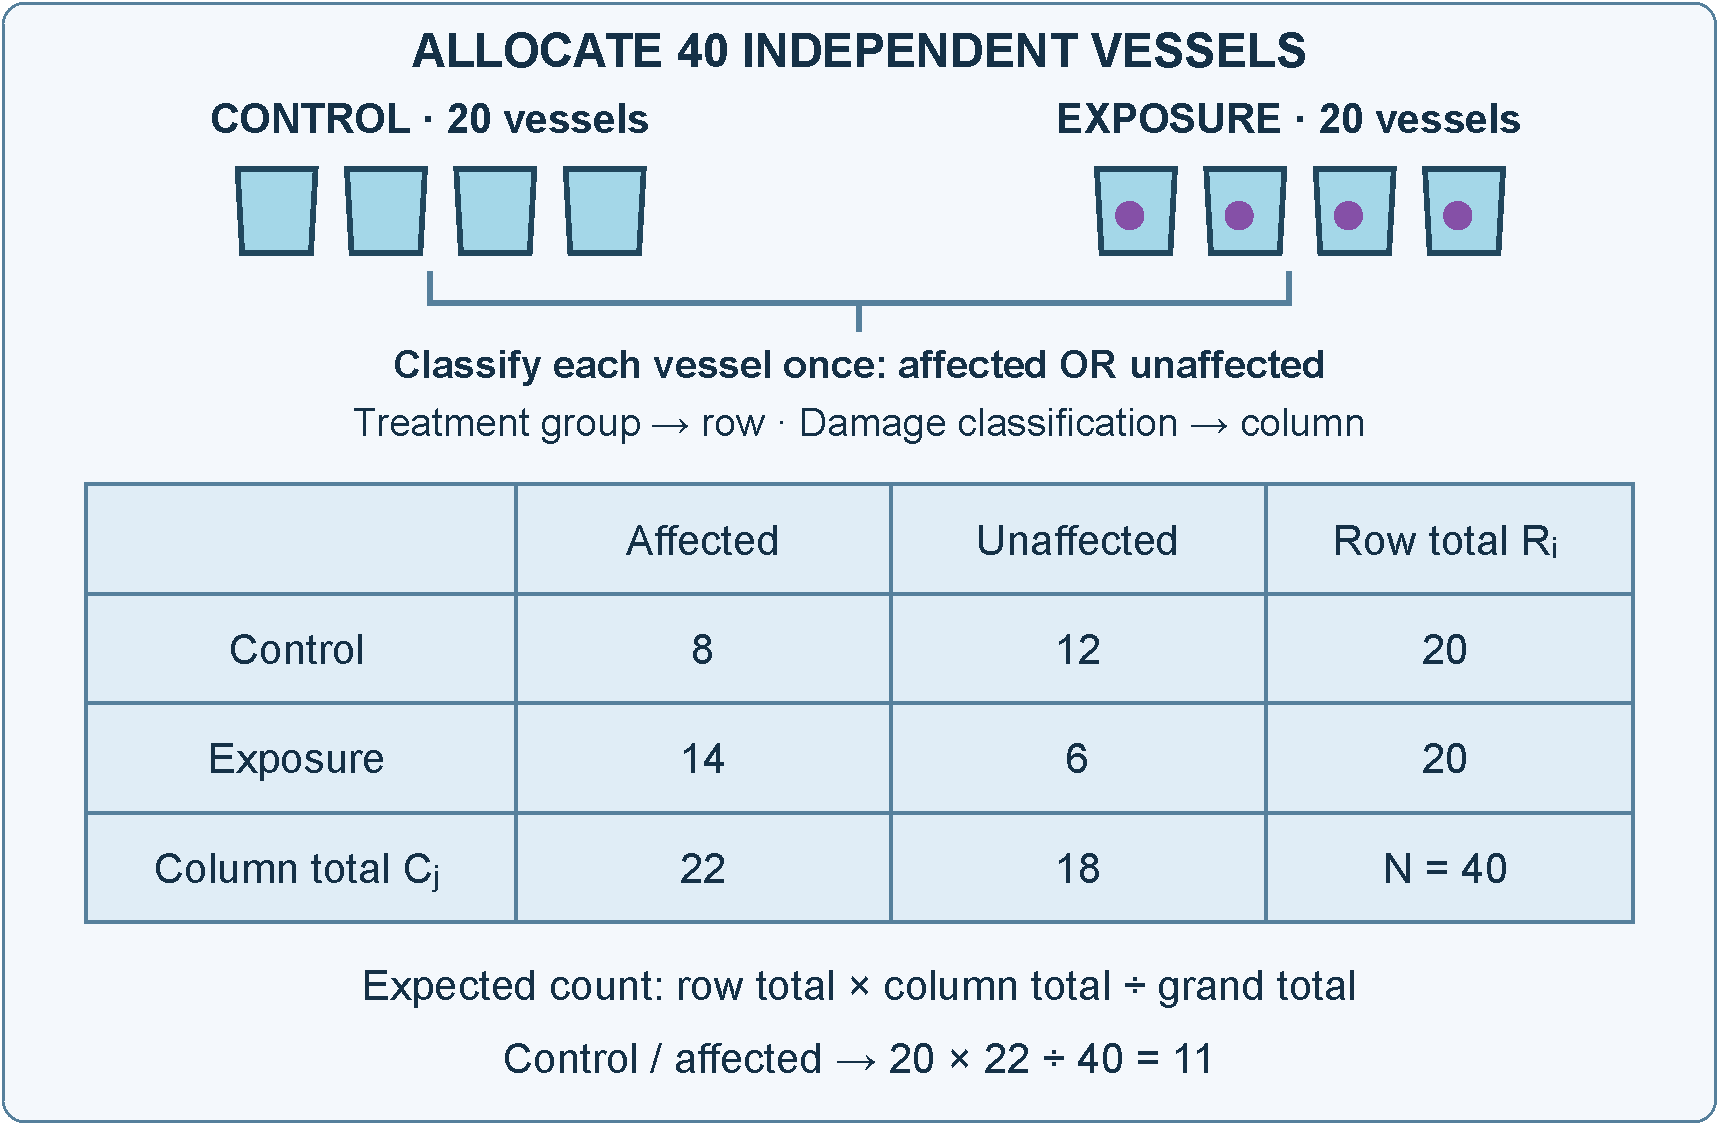
\includegraphics[width=\linewidth,height=.62\textheight,keepaspectratio]{asset-810297c1a76da92544008b233a8d5adcb21d22369c0b7b0fdbdf2df7bd2c5823.pdf}\end{center}

\medskip

\par\medskip
\Needspace{10cm}
\refstepcounter{figure}\label{material-fa79b678a3fcd687e0612266a93c9d5643681383321fc7ff5edb17686a8b8cf4}
\noindent\textbf{Fig.~\ref*{material-fa79b678a3fcd687e0612266a93c9d5643681383321fc7ff5edb17686a8b8cf4}.} NIST: known-variance test.\par\nopagebreak
\noindent\href{https://www.itl.nist.gov/div898/handbook/eda/section3/eda358.htm}{NIST: known-variance chi-square test}\par
\nolinkurl{https://www.itl.nist.gov/div898/handbook/eda/section3/eda358.htm}\par

\medskip

\par\medskip
\Needspace{10cm}
\refstepcounter{figure}\label{material-0020ebecabbc6660c149fbc34b9fff41ea856c0c43274464936460915f0429d0}
\noindent\textbf{Fig.~\ref*{material-0020ebecabbc6660c149fbc34b9fff41ea856c0c43274464936460915f0429d0}.} NIST: goodness-of-fit reference.\par\nopagebreak
\noindent\href{https://www.itl.nist.gov/div898/handbook/eda/section3/eda35f.htm}{NIST: chi-square goodness of fit}\par
\nolinkurl{https://www.itl.nist.gov/div898/handbook/eda/section3/eda35f.htm}\par

\medskip

\par\medskip
\Needspace{10cm}
\refstepcounter{figure}\label{material-1e5f142084e4de38141c9a5e144e022f873551e3b779bc3379fdd2cacac9d2ce}
\noindent\textbf{Fig.~\ref*{material-1e5f142084e4de38141c9a5e144e022f873551e3b779bc3379fdd2cacac9d2ce}.} NIST: contingency-table independence.\par\nopagebreak
\noindent\href{https://www.itl.nist.gov/div898/handbook/prc/section4/prc45.htm}{NIST: contingency-table independence}\par
\nolinkurl{https://www.itl.nist.gov/div898/handbook/prc/section4/prc45.htm}\par

\medskip

\clearpage
\section{Independent ordering and original paired differences}
Rank methods use order rather than raw mean distance, but do not remove the need to specify sampling and a null. The independent groups in \hyperref[material-0cdee2c0f7d7658c26965bd1136d7dd5489576c14e950986b7f382c5efc3a1c4]{Fig.~\ref*{material-0cdee2c0f7d7658c26965bd1136d7dd5489576c14e950986b7f382c5efc3a1c4}} contain X values 1,2,2 and Y values 2,3,4. The U statistic \hyperref[material-7393708f9720bbb98999f13258bd21ec000729b89631a40c15ca90f3ab4bd415]{Eq.~\ref*{material-7393708f9720bbb98999f13258bd21ec000729b89631a40c15ca90f3ab4bd415}} scores an X win one, a tie one half and a loss zero. The grid \hyperref[material-24d4387318f34c0e90051a12b3c9a3a91d20c11163378d47d397b8fbe9a5b193]{Fig.~\ref*{material-24d4387318f34c0e90051a12b3c9a3a91d20c11163378d47d397b8fbe9a5b193}} gives zero wins, seven losses and two ties: U for X is one. The usual null makes group labels exchangeable under equal distributions. A median-shift interpretation additionally needs the same-shaped location-shift model; differing shapes and detection-limit censoring need care.


\par\medskip
\Needspace{10cm}
\refstepcounter{figure}\label{material-0cdee2c0f7d7658c26965bd1136d7dd5489576c14e950986b7f382c5efc3a1c4}
\noindent\textbf{Fig.~\ref*{material-0cdee2c0f7d7658c26965bd1136d7dd5489576c14e950986b7f382c5efc3a1c4}.} Independent numeric groups on a shared ordered response scale.\par\nopagebreak
\begin{center}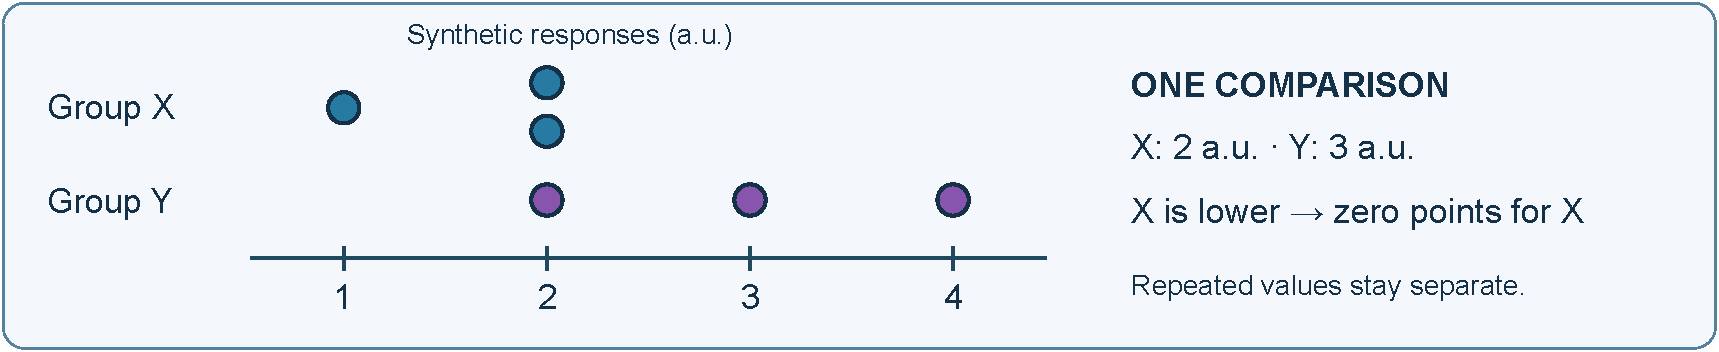
\includegraphics[width=\linewidth,height=.62\textheight,keepaspectratio]{asset-579d139afcb2afed984cd848c7431d507f74877f715ce713b27fa2806a7adae0.pdf}\end{center}

\medskip

\par\medskip
\noindent\begin{minipage}{\linewidth}
\refstepcounter{equation}\label{material-7393708f9720bbb98999f13258bd21ec000729b89631a40c15ca90f3ab4bd415}
\noindent\textbf{Eq.~\ref*{material-7393708f9720bbb98999f13258bd21ec000729b89631a40c15ca90f3ab4bd415}.} Oriented Mann–Whitney statistic with half credit for ties.\par\nopagebreak
\begin{center}\begin{adjustbox}{max width=\linewidth}$\displaystyle U_X=\sum_{i=1}^{n_X}\sum_{j=1}^{n_Y}\left[\mathbf{1}(x_i>y_j)+\tfrac12\mathbf{1}(x_i=y_j)\right]$\end{adjustbox}\end{center}

\par\noindent\textbf{Symbols}

\begin{itemize}\setlength{\itemsep}{1pt}\setlength{\parsep}{0pt}
\item \textbf{X, Y}: Independent groups on one ordered response scale.
\item \textbf{n\_X, n\_Y}: Positive group sample sizes.
\item \textbf{i, j; x\_i, y\_j}: Observation indices and their measured values.
\item \textbf{U\_X}: X wins plus half the ties; dimensionless.
\item \textbf{Bold 1(event)}: One when the condition holds, otherwise zero.
\item \textbf{>, =, +, \ensuremath{\tfrac12}}: Greater than, equal, add, half credit.
\item \textbf{Double \ensuremath{\Sigma}}: Visit every X–Y comparison.
\item \textbf{Brackets; juxtaposition}: Group terms; multiply.
\end{itemize}

Usual H\ensuremath{{}_0}: identical group distributions, exchangeable labels. This example uses an explicitly tie-aware label-permutation reference. Median-shift interpretation additionally needs common distribution shape. Software may report the complementary U.

\end{minipage}\par
\medskip

\par\medskip
\Needspace{10cm}
\refstepcounter{figure}\label{material-24d4387318f34c0e90051a12b3c9a3a91d20c11163378d47d397b8fbe9a5b193}
\noindent\textbf{Fig.~\ref*{material-24d4387318f34c0e90051a12b3c9a3a91d20c11163378d47d397b8fbe9a5b193}.} All nine cross-group comparisons; repeated observations are not merged.\par\nopagebreak
\begin{center}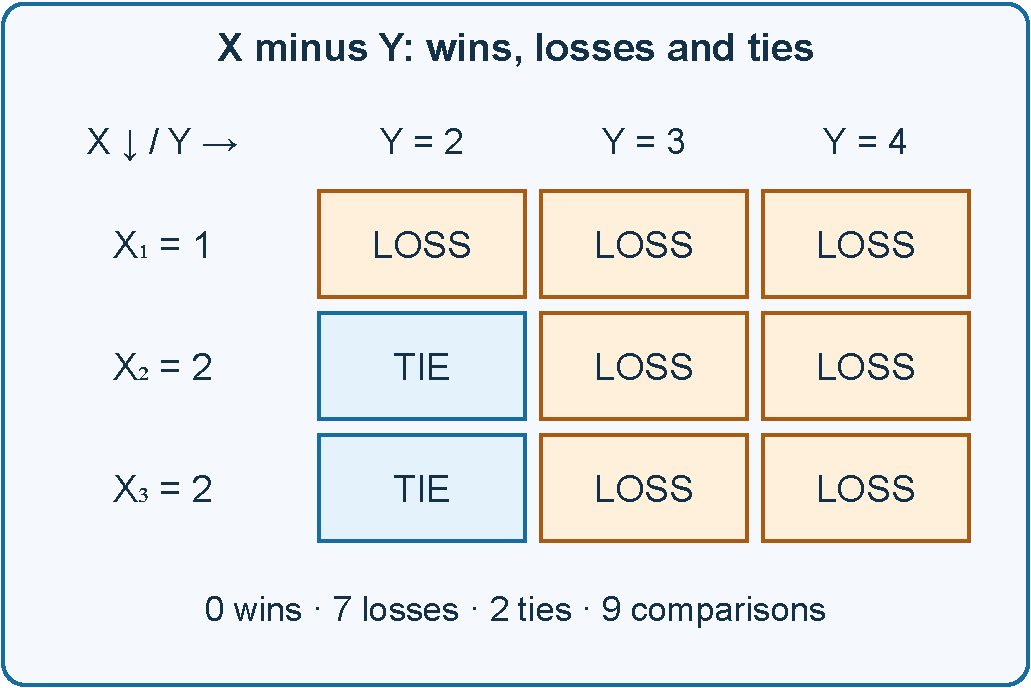
\includegraphics[width=\linewidth,height=.62\textheight,keepaspectratio]{asset-0e5b89106d914629e40b3d636cc08e46060df7aaa350d32f67bcde589252d44d.pdf}\end{center}

\medskip

The explicit tie-aware reference in \hyperref[material-4b2bb9d04828637a1b7c1ab978d737e0589ac34896857f52b2f886411c224256]{Table~\ref*{material-4b2bb9d04828637a1b7c1ab978d737e0589ac34896857f52b2f886411c224256}} enumerates all twenty assignments of three of the six observations to X, preserving tied observations as distinct units. Six assignments give U at least as far from its null centre 4.5 as the observed value one. Two-sided p is therefore 0.300, and we do not reject at 5\%. This convention is declared rather than presenting a no-tie exact table as applicable. The observed tendency for X to be smaller is descriptive, not by itself a significant distributional result.


\par\medskip
\Needspace{8\baselineskip}
\refstepcounter{scripttable}\label{material-4b2bb9d04828637a1b7c1ab978d737e0589ac34896857f52b2f886411c224256}
\noindent\textbf{Table~\ref*{material-4b2bb9d04828637a1b7c1ab978d737e0589ac34896857f52b2f886411c224256}.} Exact tie-aware two-sided label-permutation result and interpretation.\par\nopagebreak
\begin{longtable}{@{}p{\dimexpr0.500000\linewidth-2\tabcolsep\relax}p{\dimexpr0.500000\linewidth-2\tabcolsep\relax}@{}}
Field & Result \\ \hline
\endhead
Null / statistic & Equal distributions; U for X = 1; null centre 4.5 \\ \hline
Exact two-sided p & 0.300; 6 of 20 label assignments at least as far from 4.5. Tied observations retained. \\ \hline
Interpretation & X tends lower in the sample; do not reject at 5\%. Independent exchangeable labels under H\ensuremath{{}_0}; median-shift interpretation needs common shape. \\ \hline
\end{longtable}
\medskip

For paired observations, keep the original pairs. Form one \textbf{difference} per pair, then calculate the \textbf{rank of abs(diff)} using \hyperref[material-15e2d8268f1b36eb617f48e0154518cd7a40c0090579d6ece610eaf55de955c3]{Eq.~\ref*{material-15e2d8268f1b36eb617f48e0154518cd7a40c0090579d6ece610eaf55de955c3}}. Here abs means absolute value. In \hyperref[material-b4d8e4aa11c77cf416952ecd65462cf60282ea1b6785f047f714d3987a386038]{Fig.~\ref*{material-b4d8e4aa11c77cf416952ecd65462cf60282ea1b6785f047f714d3987a386038}}, differences \textbf{1,\ensuremath{-}2,3,4,5 µg/L} give \textbf{W\ensuremath{{}^+} = 13} and negative-rank sum \textbf{2}. Under the symmetric zero-shift H\ensuremath{{}_0}, each independent difference has two equally likely signs. Five choices give \textbf{2 \ensuremath{\times} 2 \ensuremath{\times} 2 \ensuremath{\times} 2 \ensuremath{\times} 2 = 32 patterns}. The total rank sum is \textbf{15} and the null centre \textbf{7.5}. Three patterns give \textbf{W\ensuremath{{}^+} \ensuremath{\le} 2}, and three give \textbf{W\ensuremath{{}^+} \ensuremath{\ge} 13}: \textbf{p = 6/32 = 0.1875}, as reported in \hyperref[material-15bcc6d54d6afaa1f2b21eef6987a1e5a95c79bac65e78479c0dee5a83767991]{Table~\ref*{material-15bcc6d54d6afaa1f2b21eef6987a1e5a95c79bac65e78479c0dee5a83767991}}. At 5\%, do not reject H\ensuremath{{}_0}. State zero and tie conventions in software.


\par\medskip
\noindent\begin{minipage}{\linewidth}
\refstepcounter{equation}\label{material-15e2d8268f1b36eb617f48e0154518cd7a40c0090579d6ece610eaf55de955c3}
\noindent\textbf{Eq.~\ref*{material-15e2d8268f1b36eb617f48e0154518cd7a40c0090579d6ece610eaf55de955c3}.} Signed ranks of original within-pair differences, not independently sorted samples.\par\nopagebreak
\begin{center}\begin{adjustbox}{max width=\linewidth}$\displaystyle d_i=x_i-y_i,\qquad W^+=\sum_{i:d_i>0}\operatorname{rank}(|d_i|)$\end{adjustbox}\end{center}

\par\noindent\textbf{Symbols}

\begin{itemize}\setlength{\itemsep}{1pt}\setlength{\parsep}{0pt}
\item \textbf{i}: Original independent pair identity, not sorted-value position.
\item \textbf{x\_i, y\_i; d\_i}: Pair readings and their first-minus-second difference; same response unit.
\item \textbf{|d\_i|}: Absolute difference size.
\item \textbf{rank}: Rank nonzero absolute differences; average ranks for ties.
\item \textbf{W\ensuremath{{}^+}}: Sum of ranks of positive differences; dimensionless. Superscript + labels this sum.
\item \textbf{\ensuremath{\Sigma}; colon}: Sum over indices satisfying the condition; such that.
\item \textbf{>, \ensuremath{-}, =}: Strictly positive comparison, subtract, equal.
\item \textbf{Parentheses}: Group the rank argument.
\end{itemize}

Usual shift inference requires independent symmetric differences. Remove zeros before ranking in this convention. Do not independently sort X and Y. Declare tie/zero handling and exact versus approximate calculation.

\end{minipage}\par
\medskip

\par\medskip
\Needspace{10cm}
\refstepcounter{figure}\label{material-b4d8e4aa11c77cf416952ecd65462cf60282ea1b6785f047f714d3987a386038}
\noindent\textbf{Fig.~\ref*{material-b4d8e4aa11c77cf416952ecd65462cf60282ea1b6785f047f714d3987a386038}.} Five independent paired differences become signed size ranks.\par\nopagebreak
\begin{center}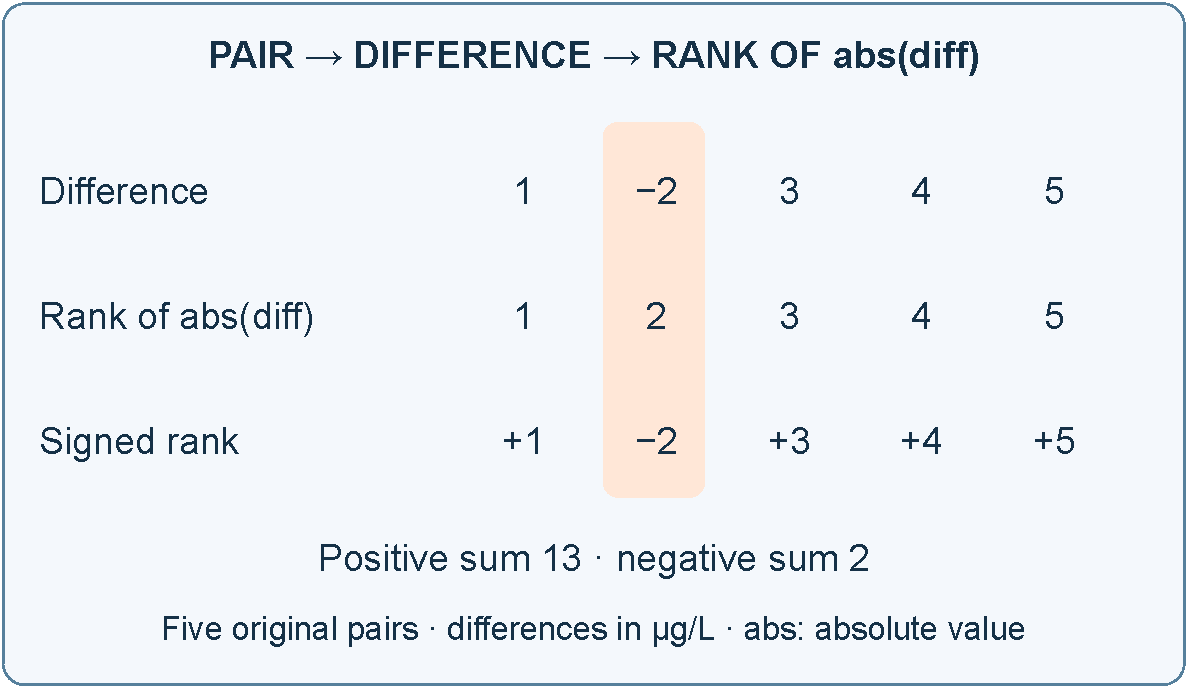
\includegraphics[width=\linewidth,height=.62\textheight,keepaspectratio]{asset-ec48d8f36e8d24c6e5b5e8982be38e9560d5a56ed8e5360a9fcb28fd599f025d.pdf}\end{center}

\medskip

\par\medskip
\Needspace{8\baselineskip}
\refstepcounter{scripttable}\label{material-15bcc6d54d6afaa1f2b21eef6987a1e5a95c79bac65e78479c0dee5a83767991}
\noindent\textbf{Table~\ref*{material-15bcc6d54d6afaa1f2b21eef6987a1e5a95c79bac65e78479c0dee5a83767991}.} Exact signed-rank report with symmetric-difference assumptions.\par\nopagebreak
\begin{longtable}{@{}p{\dimexpr0.500000\linewidth-2\tabcolsep\relax}p{\dimexpr0.500000\linewidth-2\tabcolsep\relax}@{}}
Field & Result \\ \hline
\endhead
Null / statistic & Symmetric zero-shift differences; positive-rank sum 13, negative sum 2 \\ \hline
Exact two-sided p & 0.1875; 6 of 32 sign assignments; no zeros or absolute ties \\ \hline
Decision / units & Do not reject at 5\%. Five independent paired changes in µg/L; symmetry required for the usual shift inference. Do not sort the two raw samples separately. \\ \hline
\end{longtable}
\medskip

Try the reusable compare–score–accumulate interaction \hyperref[material-f5bdc16a997cdf37776974f0d328965bbf073efcbb7a77ff44b4e8651c8dcd36]{Fig.~\ref*{material-f5bdc16a997cdf37776974f0d328965bbf073efcbb7a77ff44b4e8651c8dcd36}} before reading the grid. Each click brings one original X/Y pair together and credits the X account. The NIST rank-sum \hyperref[material-005f206c278578a859e66ca141dceebdf3344829477b9ee29f28cf4fe3d1db17]{Fig.~\ref*{material-005f206c278578a859e66ca141dceebdf3344829477b9ee29f28cf4fe3d1db17}} and signed-rank \hyperref[material-98855e877a41a0e97fae5554588a8c8076c2c03d0cbf676181492eb0629a4a4c]{Fig.~\ref*{material-98855e877a41a0e97fae5554588a8c8076c2c03d0cbf676181492eb0629a4a4c}} pages provide further reading; software statistic orientation and tie conventions can differ. Our declared tie-aware label-permutation calculation remains the reference for this U example.


\par\medskip
\Needspace{10cm}
\refstepcounter{figure}\label{material-f5bdc16a997cdf37776974f0d328965bbf073efcbb7a77ff44b4e8651c8dcd36}
\noindent\textbf{Fig.~\ref*{material-f5bdc16a997cdf37776974f0d328965bbf073efcbb7a77ff44b4e8651c8dcd36}.} Compare one pair, credit its points, accumulate U.\par\nopagebreak
\begin{center}
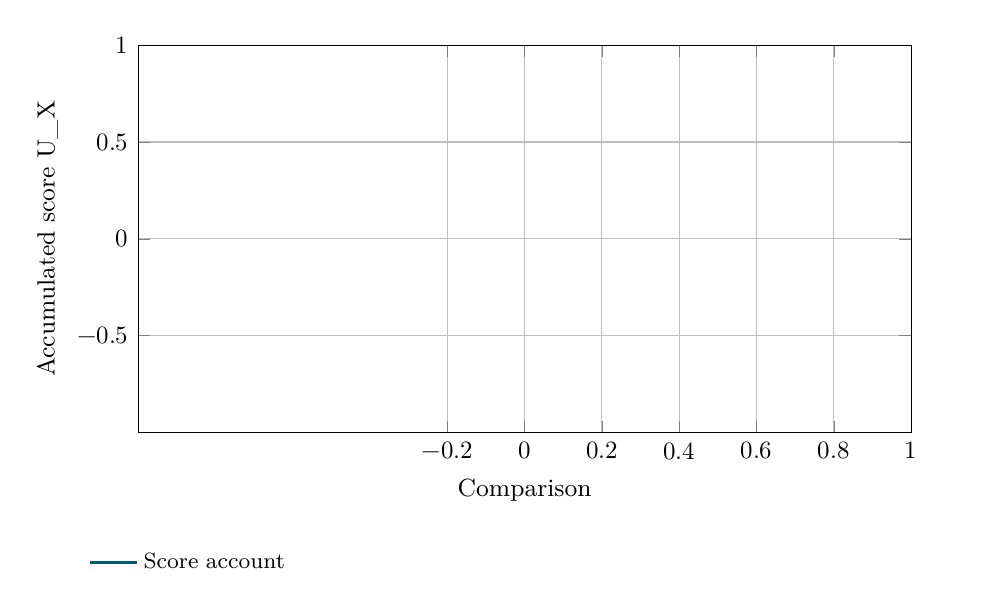
\begin{tikzpicture}
\begin{axis}[width=0.94\linewidth,
height=6.5cm,
scale only axis=false,
grid=major,
tick label style={font=\small},
label style={font=\small},
xlabel={Comparison},
ylabel={Accumulated score U\_X},
legend style={font=\footnotesize,draw=none,at={(0.5,-0.28)},anchor=north,legend columns=1,text width=0.85\linewidth,align=left},
unbounded coords=jump,
scaled ticks=false]
\addplot[color=pcd1,thick,mark=none] coordinates {(0,0)};
\addlegendentry{Score account}

\end{axis}
\end{tikzpicture}
\end{center}

% Full-precision experiment details: {"blockId":"ex:l6s-pair-chart--block","parameters":[{"key":"step","label":"Completed comparisons","value":0}],"readouts":[{"label":"Completed comparisons","value":0},{"label":"Score U_X","value":0}],"note":"1. X₁ (1) < Y₁ (2): +0; account 0\n2. X₁ (1) < Y₂ (3): +0; account 0\n3. X₁ (1) < Y₃ (4): +0; account 0\n4. X₂ (2) = Y₁ (2): +0.5; account 0.5\n5. X₂ (2) < Y₂ (3): +0; account 0.5\n6. X₂ (2) < Y₃ (4): +0; account 0.5\n7. X₃ (2) = Y₁ (2): +0.5; account 1\n8. X₃ (2) < Y₂ (3): +0; account 1\n9. X₃ (2) < Y₃ (4): +0; account 1","markers":[[]]}

\medskip

\par\medskip
\Needspace{10cm}
\refstepcounter{figure}\label{material-005f206c278578a859e66ca141dceebdf3344829477b9ee29f28cf4fe3d1db17}
\noindent\textbf{Fig.~\ref*{material-005f206c278578a859e66ca141dceebdf3344829477b9ee29f28cf4fe3d1db17}.} NIST rank sum: check statistic orientation and tie conventions.\par\nopagebreak
\noindent\href{https://www.itl.nist.gov/div898/software/dataplot/refman1/auxillar/ranksum.htm}{NIST: rank-sum test (software conventions differ)}\par
\nolinkurl{https://www.itl.nist.gov/div898/software/dataplot/refman1/auxillar/ranksum.htm}\par

\medskip

\par\medskip
\Needspace{10cm}
\refstepcounter{figure}\label{material-98855e877a41a0e97fae5554588a8c8076c2c03d0cbf676181492eb0629a4a4c}
\noindent\textbf{Fig.~\ref*{material-98855e877a41a0e97fae5554588a8c8076c2c03d0cbf676181492eb0629a4a4c}.} NIST: signed-rank test.\par\nopagebreak
\noindent\href{https://www.itl.nist.gov/div898/software/dataplot/refman1/auxillar/signrank.htm}{NIST: signed-rank test}\par
\nolinkurl{https://www.itl.nist.gov/div898/software/dataplot/refman1/auxillar/signrank.htm}\par

\medskip

\clearpage
\section{Effect magnitudes and their interpretation}
A \textbf{p-value} assesses compatibility with the null model. \textbf{Effect magnitude} describes the size of the observed difference. Start with the original units: NIR minus HPLC-MS is \textbf{\ensuremath{-}5 µg/L}. The sampling design limits the scope of inference.


Cohen's d in \hyperref[material-ecf0cc7bf7bcc20437868a7f27eb92f88150325125202f6017e52113ac90a4fb]{Eq.~\ref*{material-ecf0cc7bf7bcc20437868a7f27eb92f88150325125202f6017e52113ac90a4fb}} divides the independent-group mean difference by pooled within-group descriptive SD. Here \textbf{d = \ensuremath{-}1.677}: NIR reads lower and the mean difference is about \textbf{1.68 pooled SDs}. The reference table \hyperref[material-d435963b3a8d4369e05f348a5f35ad93d2b99c20d2f875481292ac527e0e4407]{Table~\ref*{material-d435963b3a8d4369e05f348a5f35ad93d2b99c20d2f875481292ac527e0e4407}} classifies absolute d: below \textbf{0.2 negligible}, \textbf{0.2 to below 0.5 small}, \textbf{0.5 to below 0.8 medium}, and \textbf{at least 0.8 large}. Our result is \textbf{large} by this convention. These effsize-manual bands describe a standardised magnitude; chemical relevance depends on the application. The mean inference remains Welch.


\par\medskip
\noindent\begin{minipage}{\linewidth}
\refstepcounter{equation}\label{material-ecf0cc7bf7bcc20437868a7f27eb92f88150325125202f6017e52113ac90a4fb}
\noindent\textbf{Eq.~\ref*{material-ecf0cc7bf7bcc20437868a7f27eb92f88150325125202f6017e52113ac90a4fb}.} Native-unit mean difference and descriptive pooled-SD Cohen's d.\par\nopagebreak
\begin{center}\begin{adjustbox}{max width=\linewidth}$\displaystyle \widehat\Delta=\bar x-\bar y,\qquad d=\frac{\bar x-\bar y}{s_p}$\end{adjustbox}\end{center}

\par\noindent\textbf{Symbols}

\begin{itemize}\setlength{\itemsep}{1pt}\setlength{\parsep}{0pt}
\item \textbf{Δ̂}: Estimated X-minus-Y mean difference; hat marks estimation.
\item \textbf{\ensuremath{\bar{x}}, \ensuremath{\bar{y}}}: Independent-group means; here NIR and HPLC-MS in µg/L.
\item \textbf{s\ensuremath{{}_p}}: Pooled within-group sample SD; positive square root of variance weighted by residual degrees of freedom; µg/L.
\item \textbf{d}: Uncorrected dimensionless Cohen effect estimate.
\item \textbf{p subscript}: Labels pooling.
\item \textbf{\ensuremath{-}, =, fraction bar}: Subtract, equal, divide.
\end{itemize}

Here pooling defines a descriptive standardisation. The mean test remains Welch. Magnitude guides are conventions; report native units, uncertainty and design. Paired effects use other denominators.

\end{minipage}\par
\medskip

\par\medskip
\Needspace{8\baselineskip}
\refstepcounter{scripttable}\label{material-d435963b3a8d4369e05f348a5f35ad93d2b99c20d2f875481292ac527e0e4407}
\noindent\textbf{Table~\ref*{material-d435963b3a8d4369e05f348a5f35ad93d2b99c20d2f875481292ac527e0e4407}.} Conventional bands for absolute Cohen d.\par\nopagebreak
\begin{longtable}{@{}p{\dimexpr0.500000\linewidth-2\tabcolsep\relax}p{\dimexpr0.500000\linewidth-2\tabcolsep\relax}@{}}
Absolute Cohen d & Conventional description \\ \hline
\endhead
Below 0.2 & Negligible \\ \hline
0.2 to below 0.5 & Small \\ \hline
0.5 to below 0.8 & Medium \\ \hline
0.8 or more & Large \\ \hline
\end{longtable}
\medskip

Cliff's delta in \hyperref[material-850da78ab77726879e050f35ea7204c2679076be87123929421dea59f1458d2e]{Eq.~\ref*{material-850da78ab77726879e050f35ea7204c2679076be87123929421dea59f1458d2e}} is the balance of cross-group wins and losses divided by every comparison, including ties. Our earlier grid gives \ensuremath{-}7/9, about \ensuremath{-}0.778, indicating X tends lower. Conventional absolute-delta bands are below 0.147 negligible, 0.147 to below 0.33 small, 0.33 to below 0.474 medium, and at least 0.474 large, following the Romano thresholds documented in effsize. They do not set significance or practical-relevance criteria. Comparisons reuse original observations, so uncertainty estimation must respect the independent units, not pretend there are nine independent observations.


\par\medskip
\noindent\begin{minipage}{\linewidth}
\refstepcounter{equation}\label{material-850da78ab77726879e050f35ea7204c2679076be87123929421dea59f1458d2e}
\noindent\textbf{Eq.~\ref*{material-850da78ab77726879e050f35ea7204c2679076be87123929421dea59f1458d2e}.} Cliff's delta from oriented wins, losses and the tie-aware U convention.\par\nopagebreak
\begin{center}\begin{adjustbox}{max width=\linewidth}$\displaystyle \widehat\delta=\frac{N_>-N_<}{n_X n_Y}=\frac{2U_X}{n_X n_Y}-1$\end{adjustbox}\end{center}

\par\noindent\textbf{Symbols}

\begin{itemize}\setlength{\itemsep}{1pt}\setlength{\parsep}{0pt}
\item \textbf{\ensuremath{\delta}̂}: Estimated dimensionless Cliff effect from \ensuremath{-}1 to 1; hat marks estimation.
\item \textbf{N\_>, N\_<}: Counts of X-over-Y wins and losses.
\item \textbf{n\_X, n\_Y}: Positive independent-group sample sizes.
\item \textbf{U\_X}: X wins plus half the ties.
\item \textbf{>, <}: Strictly greater and smaller comparisons.
\item \textbf{2; \ensuremath{-}; =; fraction bars}: Twice, subtract, equal, divide.
\item \textbf{Juxtaposition}: Multiply sample sizes.
\end{itemize}

Ties add zero to the signed balance but stay in the denominator. Positive delta means X tends larger. Pairs sharing observations are dependent; uncertainty follows the original independent units, not the number of comparisons.

\end{minipage}\par
\medskip

\clearpage
\section{A Grubbs flag starts an investigation}
Five nitrate results are near ten mg/L and one is 12.5. Preparation errors, contamination, instrument behaviour and genuine pollution events can all produce unusual observations. The investigation picture \hyperref[material-fb5695f6259cc7d60c6e3c3e0d6c0501fbd1d3468008dd4d66a167d4277e6512]{Fig.~\ref*{material-fb5695f6259cc7d60c6e3c3e0d6c0501fbd1d3468008dd4d66a167d4277e6512}} begins with keeping the raw value and its sample identity. Check acquisition order, blanks, calibration and preparation records rather than starting with deletion.


\par\medskip
\Needspace{10cm}
\refstepcounter{figure}\label{material-fb5695f6259cc7d60c6e3c3e0d6c0501fbd1d3468008dd4d66a167d4277e6512}
\noindent\textbf{Fig.~\ref*{material-fb5695f6259cc7d60c6e3c3e0d6c0501fbd1d3468008dd4d66a167d4277e6512}.} Keep, investigate and explain the high nitrate result.\par\nopagebreak
\begin{center}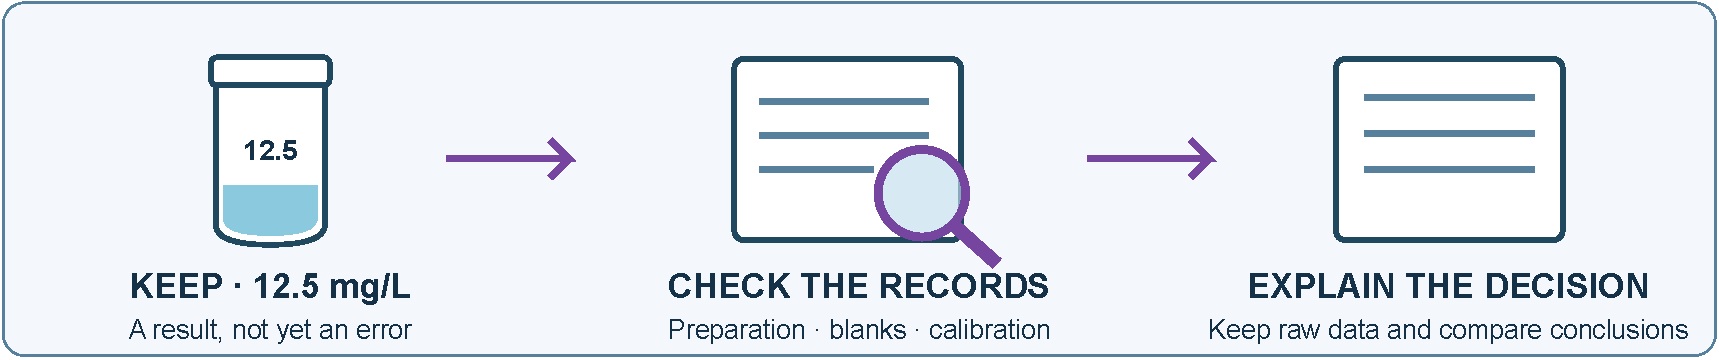
\includegraphics[width=\linewidth,height=.62\textheight,keepaspectratio]{asset-6219407362546b9b4b0603029ed31b85bdce39f7f74e6147c7dae5cd7bcf7740.pdf}\end{center}

\medskip

Grubbs' statistic \hyperref[material-583f5539b4af7f182da5ec5c427bfaf9483ce1ec158c2335a9e0caec09c326bd]{Eq.~\ref*{material-583f5539b4af7f182da5ec5c427bfaf9483ce1ec158c2335a9e0caec09c326bd}} divides the largest absolute deviation from the sample mean by sample SD, calculated from all six original results. Its null is an independent Normal sample, with an alternative concerning one extreme. The two-sided critical construction \hyperref[material-b9d4fad7495c9ff3b6cd26863ef5bc9d140322960b94c08bd0a3806f5dab50d3]{Eq.~\ref*{material-b9d4fad7495c9ff3b6cd26863ef5bc9d140322960b94c08bd0a3806f5dab50d3}} accounts for searching the complete sample. For 9.8,9.9,10.0,10.1,10.2,12.5 mg/L, G is about 2.0219 and the 5\% cutoff about 1.8871. Compare observed statistic with critical value, just as other tests compare a statistic with a reference rejection region.


\par\medskip
\noindent\begin{minipage}{\linewidth}
\refstepcounter{equation}\label{material-583f5539b4af7f182da5ec5c427bfaf9483ce1ec158c2335a9e0caec09c326bd}
\noindent\textbf{Eq.~\ref*{material-583f5539b4af7f182da5ec5c427bfaf9483ce1ec158c2335a9e0caec09c326bd}.} Observed Grubbs statistic from the complete original sample.\par\nopagebreak
\begin{center}\begin{adjustbox}{max width=\linewidth}$\displaystyle G=\frac{\max_{1\le i\le n}|x_i-\bar x|}{s}$\end{adjustbox}\end{center}

\par\noindent\textbf{Symbols}

\begin{itemize}\setlength{\itemsep}{1pt}\setlength{\parsep}{0pt}
\item \textbf{G}: Observed dimensionless maximum standardised deviation.
\item \textbf{n; i}: Sample size, at least three; observation index.
\item \textbf{x\_i; \ensuremath{\bar{x}}; s}: Observation, sample mean, positive sample SD; all mg/L.
\item \textbf{max; 1 \ensuremath{\le} i \ensuremath{\le} n}: Select the largest value over the complete sample.
\item \textbf{| |}: Absolute magnitude; checks either extreme.
\item \textbf{\ensuremath{-}, =, fraction bar}: Subtract, equal, divide.
\end{itemize}

Use all original values to compute mean and SD; sample SD uses denominator n \ensuremath{-} 1. H\ensuremath{{}_0} is an independent Normal sample; the alternative concerns one extreme. The cutoff accounts for selecting the maximum.

\end{minipage}\par
\medskip

\par\medskip
\noindent\begin{minipage}{\linewidth}
\refstepcounter{equation}\label{material-b9d4fad7495c9ff3b6cd26863ef5bc9d140322960b94c08bd0a3806f5dab50d3}
\noindent\textbf{Eq.~\ref*{material-b9d4fad7495c9ff3b6cd26863ef5bc9d140322960b94c08bd0a3806f5dab50d3}.} Selection-aware two-sided critical value and full symbol definitions.\par\nopagebreak
\begin{center}\begin{adjustbox}{max width=\linewidth}$\displaystyle \begin{gathered}c=t_{1-\alpha/(2n),n-2}\\G_{\mathrm{crit}}=\frac{n-1}{\sqrt n}\sqrt{\frac{c^2}{n-2+c^2}}\end{gathered}$\end{adjustbox}\end{center}

\par\noindent\textbf{Symbols}

\begin{itemize}\setlength{\itemsep}{1pt}\setlength{\parsep}{0pt}
\item \textbf{n}: Number of observations, at least three.
\item \textbf{\ensuremath{\alpha}}: Prespecified two-sided significance level.
\item \textbf{t\_(q,\ensuremath{\nu})}: t quantile at cumulative probability q and degrees of freedom \ensuremath{\nu}.
\item \textbf{q; \ensuremath{\nu}}: Here 1 minus alpha divided by twice n; n minus two degrees of freedom.
\item \textbf{c}: Abbreviation for that dimensionless quantile.
\item \textbf{G\_crit}: Dimensionless Grubbs cutoff; crit labels the threshold.
\item \textbf{2; \ensuremath{\sqrt{\vphantom{x}}}}: Squaring; positive square root.
\item \textbf{+, \ensuremath{-}, =, fraction bars}: Add, subtract, equal, divide.
\end{itemize}

Juxtaposition multiplies; parentheses group. Reject if G exceeds G\_crit under the independent Normal single-outlier model. This is a two-sided cutoff; one-sided procedures use a different allocation.

\end{minipage}\par
\medskip

Since G exceeds its cutoff, flag \textbf{12.5 mg/L} under this model. A flag starts an investigation. Preserve the raw record and document any scientifically justified correction or exclusion. NIST explains the single-outlier reference in \hyperref[material-714044e77e184662f842f6ed1a4f0173c8bbf4f8cd34b665ea09d74076bb24e8]{Fig.~\ref*{material-714044e77e184662f842f6ed1a4f0173c8bbf4f8cd34b665ea09d74076bb24e8}}.


\par\medskip
\Needspace{10cm}
\refstepcounter{figure}\label{material-714044e77e184662f842f6ed1a4f0173c8bbf4f8cd34b665ea09d74076bb24e8}
\noindent\textbf{Fig.~\ref*{material-714044e77e184662f842f6ed1a4f0173c8bbf4f8cd34b665ea09d74076bb24e8}.} NIST: single-outlier Grubbs test.\par\nopagebreak
\noindent\href{https://www.itl.nist.gov/div898/handbook/eda/section3/eda35h1.htm}{NIST: Grubbs single-outlier test}\par
\nolinkurl{https://www.itl.nist.gov/div898/handbook/eda/section3/eda35h1.htm}\par

\medskip

For several suspected outliers, plan a \textbf{multiple-outlier procedure}. Generalized ESD \hyperref[material-324b05aabe9ed6afebf1bccc13767889a025f581bb51f63510223b4b61518048]{Fig.~\ref*{material-324b05aabe9ed6afebf1bccc13767889a025f581bb51f63510223b4b61518048}} needs an upper bound \textbf{r} chosen before testing, an approximately Normal background, and its own adjusted sequential critical values. It calculates successive extreme-deviation statistics and selects the largest qualifying step. Repeated unadjusted Grubbs deletion changes error behaviour; a simple Bonferroni adjustment alone does not resolve adaptive deletion and masking. NIST reports reasonable critical-value approximation from \textbf{n \ensuremath{\ge} 15}, stronger from \textbf{n \ensuremath{\ge} 25}. The six-point example above remains a single-outlier illustration.


\par\medskip
\Needspace{10cm}
\refstepcounter{figure}\label{material-324b05aabe9ed6afebf1bccc13767889a025f581bb51f63510223b4b61518048}
\noindent\textbf{Fig.~\ref*{material-324b05aabe9ed6afebf1bccc13767889a025f581bb51f63510223b4b61518048}.} NIST: Generalized ESD procedure and sample-size cautions.\par\nopagebreak
\noindent\href{https://www.itl.nist.gov/div898/handbook/eda/section3/eda35h3.htm}{NIST: Generalized ESD for several outliers}\par
\nolinkurl{https://www.itl.nist.gov/div898/handbook/eda/section3/eda35h3.htm}\par

\medskip

\end{document}
